%%
% BIThesis 研究生学位论文模板 The BIThesis Template for Graduate Thesis
% This file has no copyright assigned and is placed in the Public Domain.
% Compile with: xelatex -> biber -> xelatex -> xelatex
%%

% 请勿删除下面两行注释，以免影响编译。
% !TeX program = xelatex
% !BIB program = biber

% 为方便您填写内容，模板注释会引用《撰写规范》。该文件是指研函〔2026〕024 号《北京理工大学研究生学位论文撰写规范》，可从以下链接下载。
% https://grd.bit.edu.cn/xwgz/xwgz2/wjxz_xwgz/b117825.htm

\documentclass[type=master,twoside=false]{bithesis}

\BITSetup{
  cover = {
    date = 2026年6月,
    autoWidthPadding = 0.25em,
  },
  info = {
    classification = TQ028.1,
    UDC = 540,
    title = 基于区块链的天基网络可信协同计算技术研究,
    titleEn = {Blockchain-Based Trusted Collaborative Computing Technology for Space-Based Networks},
    author = 毛心璐,
    authorEn = Xinlu Mao,
    studentId = 3220231823,
    school = 网络空间安全学院,
    schoolEn = School of Network Space Security,
    supervisor = 朱超,
    supervisorEn = Prof. Zhu Chao,
    chairman = 张涛,
    chairmanEn = Prof. Zhang Tao,
    degreeType = professional,
    industrialMentor = 朱超,
    industrialMentorEn = Prof. Zhu Chao,
    degree = 工学硕士,
    degreeEn = {Master of Engineering},
    major = 网络与信息安全,
    majorEn = Network and Information Security,
    submissionDate = 2026年6月,
    submissionDateEn = {June, 2026},
    keywords = {区块链；卫星网络；强化学习；计算卸载；联邦学习},
    keywordsEn = {Blockchain; Satellite Network; Reinforcement Learning; Computing Offloading; Federated Learning},
  },
  TOC = {
    abstract = false,
    abstractEn = false,
    symbols = false,
  },
  style = {
    pageVerticalAlign = top,
  },
  publications = {
    maxbibnames = 10,
    minbibnames = 10,
    sorting = false,
  },
  appendices / chapterLevel = true,
  misc = {
    hideLinks = true,
    tabularRowSeparation = 1.6,
  },
}

\usepackage[
  defernumbers=true,
  backend=biber,
  style=gb7714-2015,
  gbalign=gb7714-2015,
  gbnamefmt=lowercase,
  gbpub=false,
  gbannote=true,
  gbpunctin=false,
  doi=false,
  url=false,
  eprint=false,
  isbn=false,
]{biblatex}

\addbibresource{reference/main.bib}
\addbibresource{reference/pub.bib}

\usepackage{graphicx}
\usepackage{longtable}
\usepackage{array}
\usepackage{tabularx}
\usepackage{booktabs}
\usepackage{float}
\usepackage{bm}
\usepackage{algorithm}
\usepackage{algpseudocode}

\usepackage{graphicx}
\usepackage{booktabs}
\usepackage{multirow}
\usepackage{makecell}
\usepackage{float}
\usepackage{subcaption}
\usepackage[table]{xcolor}
\definecolor{bestcolor}{HTML}{F0D0D0}
\definecolor{secondcolor}{HTML}{D0E8F0}

\newcolumntype{C}{>{\centering\arraybackslash}X}
\newcolumntype{Y}{>{\raggedright\arraybackslash}X}
\newcolumntype{P}[1]{>{\centering\arraybackslash}p{#1}}

\begin{document}

\MakeCover
\MakePaperBack
\MakeTitle
\MakeOriginality

%%
% BIThesis 研究生学位论文模板 The BIThesis Template for Graduate Thesis
% This file has no copyright assigned and is placed in the Public Domain.
%%

\begin{acknowledgements}

    在本论文的研究与撰写过程中，我得到了导师、课题组老师与同学们的悉心指导和帮助。导师在研究选题、技术路线设计、论文结构组织以及学术表达规范等方面给予了耐心细致的指导，使我能够逐步完成从问题分析到方法设计、再到论文整理的全过程。在此谨向导师致以诚挚的感谢。

    同时，感谢课题组各位老师和同学在研究讨论、资料整理、实验推进与论文修改过程中提供的帮助与建议。与大家的交流使我对天基网络计算卸载、区块链协同、联邦学习与强化学习等相关问题有了更加深入的理解，也为本论文的完善提供了重要支持。

    此外，感谢学校和学院提供的学习环境与科研条件，感谢家人在研究和生活过程中给予的理解、鼓励与支持。正是因为来自师长、同学与家人的帮助，我才能较为顺利地完成本阶段的学习与研究工作。

    % 既然写到这里，那估计就要大功告成了。无论过程与结果如何，总是人生一段独特体验。祝贺！
    % 如有兴趣，可填写以下反馈问卷，帮助 BIThesis 未来优化。
    % https://wj.qq.com/s2/22532808/254f/
\end{acknowledgements}


\frontmatter

\begin{abstract}
  近年来，随着天地一体化信息网络、低轨卫星星座和在轨智能处理技术的快速发展，天基网络正由传统的数据传输网络向“通信、计算、存储与智能处理一体化”的分布式协同计算网络演进。卫星节点在灾害应急通信、遥感快速处理、空间态势感知、区域目标识别和边远区域信息服务等场景中承担着越来越多高时敏、高动态和高自治需求的计算任务。然而，受星载平台体积、功耗、能量循环、计算能力和星间链路条件限制，单星本地处理难以长期支撑高并发任务负载；传统星地集中处理模式又容易受到星地链路时延、可见窗口和回传带宽约束，难以满足任务快速闭环处理需求。因此，如何在高动态、异构和去中心化的天基环境下实现可信状态共享、多节点协同资源分配、并发感知任务卸载与平台化运行支撑，已成为天基协同计算网络亟需解决的关键问题。

  针对上述挑战，本文围绕天基网络协同计算卸载问题，提出一种融合区块链、多智能体强化学习、联邦学习与深度强化学习的双层智能管控与可信协同计算卸载方法体系。该体系以区块链作为分布式可信底座，在系统层实现多节点可信状态共享、协同博弈与资源分配，在任务层实现并发开销预测和实时卸载决策，并通过平台化架构将算法模型、状态同步、任务存证、模型治理和执行反馈统一纳入可运行、可验证、可审计的闭环环境中。本文主要研究内容与创新点如下：

  （1）提出基于区块链与多智能体强化学习的天基计算网络协同资源分配方法。针对去中心化天基环境中节点自利行为、信息不完全和资源竞争导致的负载失衡问题，将系统层协同资源分配建模为多智能体马尔可夫博弈，构建区块链增强的集中训练—分散执行多智能体强化学习框架。该方法以联盟链作为可信公共信息板，维护节点负载、链路状态、信誉评分和历史行为记录等公共摘要，并设计融合任务完成质量、系统公平性与信誉激励的混合奖励机制，引导异构卫星节点在分散自治条件下实现更稳定的协同资源分配。

  （2）提出基于联邦学习与深度强化学习的并发感知任务层计算卸载方法。针对多任务并发条件下 CPU 时间片、缓存、内存带宽和 I/O 队列竞争所引发的隐性执行代价，建立任务级并发开销模型，并构建“联邦学习预测 + DQN 卸载决策”的闭环机制。该方法利用聚类式联邦学习在不上传原始任务日志的前提下训练并发开销预测模型，通过联盟链维护模型版本和可信摘要，并将预测结果、本地状态和链上公共信息共同输入深度 Q 网络，使卫星终端能够在链上状态存在时滞和节点数据异构的条件下实现低开销、实时化、具备并发风险前瞻能力的任务卸载决策。

  （3）设计面向天基协同计算的区块链平台架构与运行机制。针对系统层协同优化和任务层实时决策缺乏统一承载环境的问题，构建面向动态星地网络的区块链协同计算平台。该平台通过轻量级联盟链共识、分层链结构、链上/链下协同机制和智能合约治理体系，实现关键状态可信同步、任务行为存证、模型版本溯源、节点信誉演化和执行反馈回流。平台将系统层全局协同资源分配方法与任务层并发感知卸载方法统一映射到工程化运行环境中，支撑天基协同计算从算法验证向可信部署和持续演化转化。

  （4）开展多场景仿真与系统级验证。围绕系统层协同资源分配、任务层并发感知卸载和区块链平台运行机制，设计收敛性、负载均衡、任务完成率、时延能耗、鲁棒性、消融分析和平台功能验证等实验。实验结果表明，本文所提方法能够在高动态链路、异构节点能力、任务非平稳到达和并发执行干扰等条件下有效降低平均任务时延和系统能耗，提高任务完成率、系统吞吐量与负载均衡水平，并增强分布式环境下的状态可信性、模型可追溯性和协同稳定性。

  综上，本文面向天基协同计算网络中“可信共享—系统协同—任务决策—平台承载”的完整链路，构建了融合区块链与人工智能的协同计算卸载方法体系。相关研究为提升受限资源条件下天基网络的任务处理效率、自治协同能力和可信运行水平提供了理论依据与技术支撑，也为未来构建高效、智能、可信的天基边缘计算网络奠定了基础。
\end{abstract}

% 如需手动控制换行连字符位置，可写 aa\-bb，详见
% https://bithesis.bitnp.net/faq/hyphen.html

\begin{abstractEn}
  In recent years, with the rapid development of space-ground integrated information networks, low Earth orbit satellite constellations, and on-orbit intelligent processing technologies, space-based networks are evolving from traditional data transmission networks into distributed collaborative computing networks integrating communication, computation, storage, and intelligent processing. Satellite nodes are undertaking increasingly time-sensitive, dynamic, and autonomous computing tasks in scenarios such as disaster emergency communication, rapid remote sensing processing, space situational awareness, regional target recognition, and information services for remote areas. However, constrained by onboard platform size, power consumption, energy cycles, computing capability, and inter-satellite link conditions, local processing on a single satellite can hardly sustain intensive concurrent workloads for a long time. Meanwhile, traditional space-ground centralized processing is limited by propagation latency, visibility windows, and feeder link bandwidth, making it difficult to satisfy the requirements of fast closed-loop task processing. Therefore, how to realize trusted state sharing, multi-node collaborative resource allocation, concurrency-aware task offloading, and platform-based operation support in highly dynamic, heterogeneous, and decentralized space environments has become a key challenge for space-based collaborative computing networks.

  To address these challenges, this thesis investigates collaborative computation offloading in space-based networks and proposes a dual-layer intelligent management and trusted collaborative computation offloading framework integrating blockchain, multi-agent reinforcement learning, federated learning, and deep reinforcement learning. In this framework, blockchain serves as a distributed trusted foundation. At the system layer, it supports trusted state sharing, collaborative game modeling, and multi-node resource allocation. At the task layer, it enables concurrency overhead prediction and real-time offloading decision-making. Furthermore, a platform-oriented architecture is designed to integrate algorithm models, state synchronization, task recording, model governance, and execution feedback into an operational, verifiable, and auditable closed-loop environment. The main research contents and contributions of this thesis are summarized as follows:

  (1) A blockchain and multi-agent reinforcement learning based collaborative resource allocation method for space-based computing networks is proposed. To address load imbalance caused by selfish node behaviors, incomplete information, and resource competition in decentralized space environments, the system-layer collaborative resource allocation problem is modeled as a multi-agent Markov game. A blockchain-enhanced centralized training and decentralized execution multi-agent reinforcement learning framework is constructed. In this method, the consortium blockchain acts as a trusted public information board to maintain public summaries such as node load, link status, reputation scores, and historical behavior records. A hybrid reward mechanism incorporating task completion quality, system fairness, and reputation incentives is further designed to guide heterogeneous satellite nodes toward stable collaborative resource allocation under decentralized autonomous execution.

  (2) A federated learning and deep reinforcement learning based concurrency-aware task-layer computation offloading method is proposed. To characterize the hidden execution costs caused by CPU time slicing, cache conflicts, memory bandwidth contention, and I/O queue competition under multi-task concurrency, a task-level concurrency overhead model is established, and a closed-loop mechanism of federated learning based prediction and DQN based offloading decision-making is designed. The proposed method employs clustered federated learning to train concurrency overhead prediction models without uploading raw task logs, maintains model versions and trusted summaries through blockchain, and feeds the predicted overhead, local state, and on-chain public information into a deep Q-network. As a result, satellite terminals can make low-overhead, real-time, and forward-looking offloading decisions under delayed on-chain states and heterogeneous node data distributions.

  (3) A blockchain platform architecture and operating mechanism for space-based collaborative computing are designed. To provide a unified execution environment for system-layer collaborative optimization and task-layer real-time decision-making, a blockchain-based collaborative computing platform for dynamic space-ground networks is constructed. Through lightweight consortium blockchain consensus, hierarchical chain structures, on-chain/off-chain collaboration, and smart contract based governance, the platform realizes trusted synchronization of key states, task behavior recording, model version traceability, node reputation evolution, and execution feedback. It maps the proposed system-layer global resource allocation method and task-layer concurrency-aware offloading method into an engineering-oriented operational environment, supporting the transition from algorithm validation to trusted deployment and continuous evolution.

  (4) Multi-scenario simulations and system-level verification are carried out. Experiments are designed for system-layer collaborative resource allocation, task-layer concurrency-aware offloading, and blockchain platform operation, including convergence analysis, load balancing, task completion rate, latency and energy consumption, robustness, ablation studies, and platform function verification. Experimental results show that the proposed methods can effectively reduce average task latency and system energy consumption, improve task completion rate, system throughput, and load balancing performance, and enhance state trustworthiness, model traceability, and collaborative stability in distributed environments with highly dynamic links, heterogeneous node capabilities, non-stationary task arrivals, and concurrent execution interference.

  In summary, this thesis constructs a blockchain and artificial intelligence integrated collaborative computation offloading framework for the complete chain of trusted sharing, system collaboration, task decision-making, and platform support in space-based collaborative computing networks. The research provides theoretical foundations and technical support for improving task processing efficiency, autonomous collaboration capability, and trusted operation under resource-constrained space environments, and lays a foundation for building efficient, intelligent, and trustworthy space-based edge computing networks in the future.
\end{abstractEn}

\MakeTOC
\listoffigures
\listoftables
%%
% BIThesis 研究生学位论文模板 The BIThesis Template for Graduate Thesis
% This file has no copyright assigned and is placed in the Public Domain.
%%

\begin{symbols}
  \item[ST] 卫星终端（Satellite Terminal）
  \item[SEN] 卫星边缘节点（Satellite Edge Node）
  \item[FL] 联邦学习（Federated Learning）
  \item[DQN] 深度Q网络（Deep Q-Network）
  \item[MDP] 马尔可夫决策过程（Markov Decision Process）
  \item[$T_i$] 第 $i$ 个任务
  \item[$C_i$] 任务 $T_i$ 的计算量
  \item[$S_i$] 任务 $T_i$ 的输入数据规模
  \item[$D_i$] 任务 $T_i$ 的时延约束（截止期）
  \item[$\tau_i$] 任务类型编码
  \item[$\zeta_i$] 任务优先级
  \item[$\mathcal{A}$] 卸载动作集合
  \item[$L_i^{\mathrm{loc}}$] 任务本地执行完成时延
  \item[$E_i^{\mathrm{loc}}$] 任务本地执行能耗
  \item[$L_i^{\mathrm{off}}$] 任务卸载执行完成时延
  \item[$E_i^{\mathrm{off}}$] 任务卸载执行能耗
  \item[$R_{i,n}^{\mathrm{up}}$] 任务 $T_i$ 到候选节点 $n$ 的上行传输速率
  \item[$F_n$] 候选节点 $n$ 的可用计算能力
  \item[$W_{n}^{\mathrm{edge}}$] 候选节点 $n$ 的基础排队时延
  \item[$\Delta_i(n,t)$] 任务 $T_i$ 在节点 $n$ 上的并发扰动时延
  \item[$CO_i(n,t)$] 任务 $T_i$ 在节点 $n$ 上的并发开销
  \item[$J_i(a_t)$] 动作 $a_t$ 对应的单任务综合代价
  \item[$\omega_L,\omega_E,\omega_C$] 时延、能耗与并发扰动代价权重
\end{symbols}


\mainmatter

\chapter{绪论}
\label{chap:intro}
% ============================================================
\section{研究背景与意义}
% ============================================================

天地一体化信息网络是支撑未来全球通信、遥感感知、任务协同与智能服务的重要基础设施，也是推动空天信息系统由传统“数据传输网络”向“综合信息处理网络”演进的关键方向。随着低轨卫星星座持续部署、星间链路逐步完善以及星载计算平台能力不断提升，卫星节点的功能定位正在发生深刻变化。传统卫星网络更多承担透明转发与数据中继功能，而新一代天基网络则逐步具备在轨处理、任务协同、资源调度和自治管控等能力，正在由单纯的信息传输载体演进为面向复杂业务场景的分布式协同计算平台。对于天地一体化信息网络而言，这种演进不仅意味着网络服务能力的提升，也意味着网络运行模式、任务组织方式与资源管理机制的系统性变革\cite{ref1,ref2,ref3}。

从现实应用需求看，天基网络正在承担越来越多高时敏、高动态和高自治要求的业务任务。在灾害应急通信、对地观测快速处理、区域目标识别、空间态势感知、海洋与航运监测以及跨区域任务协同等场景中，系统不仅需要完成数据采集和远程传输，还需要在有限可见窗口、受限链路条件和复杂任务环境下实现任务接入、资源协调、计算处理与结果反馈的快速闭环。尤其是在突发灾害、局部冲突、复杂海域巡检等场景中，任务往往具有突发性、密集性和强时效性，若仍然依赖传统“星上初步处理—地面集中分析”的工作模式，则容易受到星地链路时延、可见窗口受限以及地面中心计算负载瓶颈等因素制约，难以满足高时敏业务对于快速响应和在轨闭环处理的实际需求\cite{ref2,ref4}。

在此背景下，将计算能力由地面向星上前移，并在多颗卫星之间实现资源共享与协同处理，已成为提升天基网络智能服务能力的重要发展方向。与仅依赖地面中心的集中处理模式相比，星上计算能够缩短数据处理链路、降低回传压力、提升任务响应速度；而进一步引入多星协同计算，则有望突破单颗卫星在算力、能量、存储和链路条件等方面的资源限制，在更大空间范围内实现任务迁移、负载分担和算力共享，从而增强天基网络在复杂动态场景下的综合服务能力。

图~\ref{fig:scenario}给出了天基网络协同计算卸载的典型应用场景。在该场景中，地面突发任务首先通过上行链路接入过载卫星，过载卫星在本地资源不足或任务积压严重时，可将部分任务经由星间链路卸载至资源相对空闲的卫星节点执行；同时，区块链/多智能体管控层对各卫星节点的资源状态、协同关系和策略执行过程进行支撑，实现状态共享、共识记账与策略协同，最终将处理结果回传地面。该图较为直观地反映了本文所关注问题的典型特征，即高动态环境下多节点之间的任务迁移、资源协调、可信共享与协同决策问题。

\begin{figure}[htbp]
  \centering
  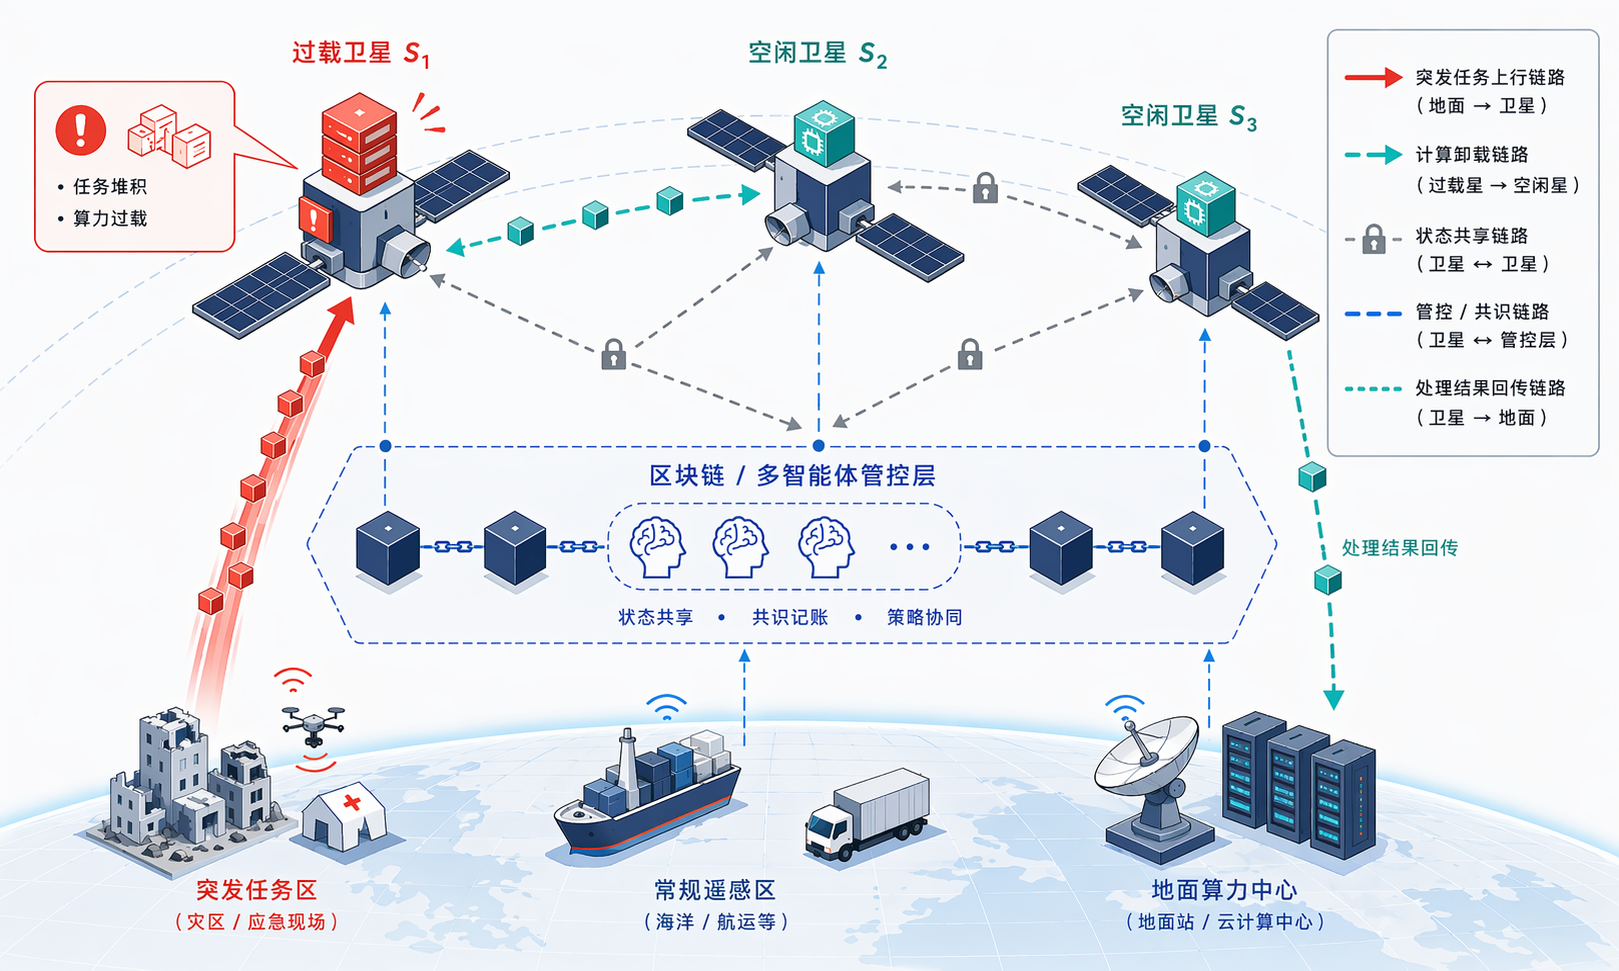
\includegraphics[width=0.85\textwidth]{figures/1-1.png}
  \caption{天基网络协同计算卸载应用场景}
  \label{fig:scenario}
\end{figure}

从现有技术体系看，面向天基网络任务处理需求，当前计算能力部署方式主要可归纳为星地集中处理、星上本地处理、星间协同处理以及分布式智能管控等几种典型模式。不同模式在支撑基础、服务能力和适用范围等方面各有特点，但同时也存在明显局限。为更清晰地说明不同模式的适用性与不足，表~\ref{tab:computing_modes}给出了典型天基网络计算模式及其技术特点对比。

\begin{table}[htbp]
  \centering
  \caption{典型天基网络计算模式及其技术特点}
  \label{tab:computing_modes}
  \begin{tabularx}{\textwidth}{CCCC}
    \toprule
    \textbf{计算模式} & \textbf{核心支撑}   & \textbf{主要能力}    & \textbf{典型局限}         \\
    \midrule
    星地集中处理        & 地面中心、馈电链路       & 适合离线分析与统一调度      & 受星地时延、可见窗口和回传带宽限制     \\
    星上本地处理        & 星载处理器、单星资源      & 支持任务就地预处理与快速响应   & 受单星算力、功耗与能量循环约束       \\
    星间协同处理        & 星间链路、多星协同       & 支持跨节点算力共享与任务迁移   & 动态拓扑下状态获取与决策复杂        \\
    分布式智能管控       & 区块链、MARL、FL、DRL & 支持可信共享、协同博弈与智能卸载 & 需同时解决共识开销、协同稳定与代价预测问题 \\
    \bottomrule
  \end{tabularx}
\end{table}

如表~\ref{tab:computing_modes}所示，星地集中处理模式依托地面中心强大的存储和计算资源，适合完成统一分析、全局调度与离线决策，但其运行效果高度依赖星地链路质量、卫星可见窗口和回传带宽条件，当任务具有强实时性要求时，该模式的闭环响应能力往往受到限制。相比之下，星上本地处理模式能够在数据产生位置附近完成预处理与快速决策，具有较好的实时性优势，但单颗卫星受平台尺寸、载荷能力、功耗预算、热控条件以及轨道能量循环等因素约束，难以长期承担高强度、连续化、多任务并发的计算需求。当任务密集到达或局部区域业务突发增长时，单节点容易出现排队积压、执行时延抬升以及任务失效等问题。

正是在上述矛盾推动下，星间协同处理逐渐成为天基网络计算能力提升的重要路径。所谓协同计算卸载，是指当任务接入卫星本地资源不足或本地执行代价过高时，通过星间链路将任务迁移至其他具备可用资源的协同节点执行，从而在更大范围内实现算力共享与负载分担\cite{ref1,ref5}。与传统纯星地集中处理模式相比，协同计算卸载能够更灵活地利用多节点资源；与单星本地处理模式相比，其能够突破单节点资源上限，在降低任务时延、提高系统吞吐量和增强网络鲁棒性方面具有明显优势。因此，协同计算卸载已成为天基网络由“可通信”向“可协同、可计算、可自治”演进过程中的关键技术之一。

然而，天基网络中的协同计算卸载并不是传统意义上的简单任务迁移问题。与地面云计算、边缘计算环境相比，天基网络中的节点资源更加受限、链路拓扑变化更加频繁、运行环境更加动态复杂。卫星高速运动使得网络拓扑、链路质量、覆盖关系和可见窗口持续变化，不同卫星节点在剩余算力、存储资源、链路状态和能量水平等方面往往存在显著异质性。与此同时，多颗卫星在同一时刻既可能是任务发起方，也可能是资源提供方，节点之间普遍存在资源竞争、收益耦合和协同行为。由此决定了天基协同计算卸载不仅要解决“任务是否卸载、卸载到哪里”的问题，更要解决高动态、去中心化环境下多节点之间的状态共享、协同博弈、实时决策与执行保障问题。

进一步而言，天基协同计算卸载的复杂性主要体现在以下几个层面。

首先，在信息层面，需要解决高动态环境下的可信状态共享问题。无论是节点间的资源协调，还是单任务的卸载决策，都依赖于对节点算力占用、剩余能量、链路连通性、队列长度和任务排队状态等信息的及时获取。然而在天基网络中，若仅依赖频繁广播实现全局状态同步，不仅会带来较大的通信开销，还可能由于链路时延、局部信息失真和同步滞后导致认知不一致。更重要的是，在去中心化的天基环境中缺乏长期稳定且可信的中心控制节点，一旦共享状态出现滞后、篡改或偏差，后续资源调度与任务卸载就可能失去可靠依据。因此，如何为多节点协同决策提供可追溯、可信任、低冲突的状态共享基础，是实现协同计算卸载的首要前提。

其次，在决策层面，需要同时面对系统层协同和任务层执行两类问题。一方面，在多颗卫星同时发起卸载请求的场景下，优质节点极易成为竞争焦点。若各节点仅从局部收益出发进行贪婪选择，则容易引发策略震荡、热点聚集、负载失衡和资源抢占等问题，影响系统整体运行效率。另一方面，任务进入目标节点后并非立即进入理想执行状态，而是会受到排队延迟、上下文切换、缓存竞争、内存争用以及功耗波动等多种并发因素影响。由此，任务层卸载决策不仅要考虑传输时延与计算时间，还需要进一步考虑更贴近真实运行环境的执行代价，才能保证卸载策略在高负载和复杂动态场景下仍具备实际有效性。

再次，在实现层面，需要解决算法方法与系统平台之间的统一承载问题。对于天基协同计算卸载而言，仅有卸载模型或优化算法并不足以支撑系统的长期稳定运行。系统层协同方法需要状态同步、规则执行、行为记录和可信审计机制作为支撑；任务层实时决策方法则依赖模型版本管理、执行反馈、结果回流以及跨节点可追溯记录。若缺乏统一的平台承载，相关方法往往停留在算法验证或离线仿真层面，难以形成可部署、可验证、可持续演进的实际运行体系。因此，从平台视角统筹考虑可信共享、协同优化、模型治理和执行反馈，同样是天基协同计算卸载研究不可回避的重要内容。

综上可见，天基协同计算卸载并不是单一节点上的局部任务调度问题，而是涉及任务接入、状态共享、跨节点协同、资源竞争、执行扰动以及结果回传等多个环节的系统性问题。该问题既具有典型的高动态、异构、去中心化特征，又包含状态可信、协同博弈和实时决策等多层耦合关系。传统依赖静态假设或中心控制的处理思路，已难以满足复杂天基环境下多节点协同计算的实际需求。因此，有必要面向可信共享、系统层协同优化、任务层实时卸载决策以及平台化承载机制开展联合研究，构建更加适应天基网络运行特征的协同计算卸载方法体系。

基于上述背景，本文围绕天基网络协同计算卸载中的关键问题展开研究，重点关注高动态环境下的可信状态共享、多节点协同资源博弈、并发感知任务卸载以及双层智能方法的平台化承载等内容。本文认为，天基协同计算卸载研究不仅在工程应用层面对提升灾害应急、遥感快处理、空间任务协同和边远区域信息服务等能力具有重要价值，而且在理论与方法层面也可为高动态、去中心化、资源受限网络环境中的分布式协同计算研究提供新的思路。通过构建兼顾可信共享、系统协同、任务决策与平台承载的统一研究框架，有望提升天基网络在复杂任务场景下的实时响应能力、资源利用效率与智能自治水平，为天地一体化信息网络向智能化、协同化和自治化方向发展提供理论支撑与技术参考。

% ============================================================
\section{国内外研究现状与发展趋势}
% ============================================================

围绕天基网络协同计算卸载问题，国内外研究已从体系架构、任务卸载、智能调度、去中心化协同、隐私保护建模以及平台化支撑等多个角度展开探索。总体来看，相关研究正沿两个方向并行推进：一方面，卫星边缘计算与星间协同处理不断走向实用化，任务卸载与资源调度问题逐步由静态建模转向动态学习；另一方面，随着网络规模扩张和节点自治能力增强，可信共享、分布式共识、联邦学习以及区块链平台等支撑机制日益成为研究重点。基于此，本节从天基边缘计算与卸载、动态环境下的智能调度、多节点可信协同与隐私保护三个方面进行梳理，并据此明确本文的研究定位。

\subsection{天基网络与卫星边缘计算研究现状}

随着低轨卫星星座的快速发展，卫星边缘计算已成为天基网络研究中的热点方向。已有研究普遍认为，未来卫星网络不应仅承担透明转发功能，而应具备在轨预处理、局部协同分析和边缘服务承载能力，以缓解地面中心压力并提升实时响应能力\cite{ref1,ref4}。围绕这一目标，学界先后提出星地协同、星间协同和天地融合等多种计算架构，试图根据任务复杂度、时延要求和资源约束，在终端、卫星与地面之间灵活划分处理位置。

在具体卸载方法方面，早期研究多采用解析优化、启发式搜索或博弈论方法，对时延、能耗和资源利用率进行联合建模。这类方法在问题规模较小且假设条件较强时具有较好的可解释性，但当网络拓扑频繁变化、链路状态动态波动或任务到达具有突发性时，其模型有效性往往难以长期保持。例如，Gao等针对LEO星座网络中的分布式动态卸载问题，基于博弈论建立了联合计算卸载与功率分配模型，在分布式环境下优化了资源利用效率，但该方法的求解过程依赖较强的信道静态假设\cite{ref19}。

自2024年以来，相关研究开始更加重视卸载问题中的时变信道、队列状态和动态负载因素。Jia等提出面向卫星边缘计算的深度多智能体强化学习方法MATORA，将任务卸载与资源分配拆分求解，在动态负载条件下提高了时延优化能力\cite{ref3}。Li等针对LEO卫星边缘计算网络研究了基于MADDPG的联合卸载与资源分配问题，通过分布式学习处理高动态环境中的能耗与时延折中\cite{ref2}。Shuai等讨论了基于Q-learning的卫星边缘计算卸载策略，进一步验证了强化学习方法在动态卫星场景中的适应性\cite{ref5}。与此同时，Tang等研究了基于星间链路的星地一体化网络任务卸载与资源分配问题，提出混合云与卫星多层多接入边缘计算架构，通过联合优化节点选择、卸载比率和算力分配实现了网络资源的动态管理\cite{ref20}。

进入2025年以后，研究重点进一步从“是否卸载”扩展到“如何在多目标条件下稳定卸载”。Xu等提出面向卫星边缘计算的多目标强化学习卸载方法，将时延、资源利用率和负载均衡纳入统一优化目标，改善了复杂任务场景下的综合性能\cite{ref15}。Ma等则着重分析了任务优先级、资源竞争和联合分配之间的耦合关系，指出卸载研究正在由单一指标优化转向优先级感知、服务质量约束和多资源联合编排\cite{ref16}。在此基础上，Wang等提出MARATD3算法，将循环神经网络与多头注意力机制引入多智能体深度确定性策略梯度框架，在部分可观测条件下实现了跨时隙的动态卸载与资源分配联合优化，为高动态卫星环境中的序贯决策问题提供了新的建模范式\cite{ref21}。与此同时，Jia等探索了联邦深度强化学习在低轨卫星边缘计算中的应用，将联邦学习与DRL相结合，在保护用户数据隐私的同时优化计算卸载策略，指出联邦学习不仅能够保护隐私，还可作为卸载策略训练的分布式支撑手段\cite{ref22}。

这些研究表明，卫星边缘计算与任务卸载已由概念验证阶段逐步迈向细粒度建模与智能优化阶段。2024—2026年天基计算卸载与智能调度领域的代表性研究如表~\ref{tab:offloading_survey}所示。

\begin{table}[htbp]
  \centering
  \caption{2024—2026年天基计算卸载与智能调度代表研究}
  \label{tab:offloading_survey}
  \begin{tabularx}{\textwidth}{cCCC}
    \toprule
    \textbf{研究方向} & \textbf{代表文献}                & \textbf{主要内容}                       & \textbf{不足或启示}                 \\
    \midrule
    卫星边缘计算架构      & \cite{ref1,ref4}             & 从星地融合、星间协同和天地一体化角度讨论卫星边缘计算架构与业务承载方式 & 侧重体系层面描述，对协同决策机制的讨论不足          \\
    \addlinespace
    博弈论与优化方法      & \cite{ref19,ref20}           & 利用博弈论、凸优化或分层架构处理卸载与资源联合分配           & 依赖较强的信道平稳或全局信息可获得假设            \\
    \addlinespace
    单智能体RL卸载      & \cite{ref5,ref15}            & 利用Q-learning、DQN及其改进模型优化卸载时延和资源利用率  & 多从单节点或单任务视角建模，难以处理多节点博弈        \\
    \addlinespace
    MARL联合优化      & \cite{ref2,ref3,ref16,ref21} & 将多颗卫星建模为多智能体，联合优化卸载、功率、带宽和资源分配      & 通常假设状态可获得，可信共享基础偏弱             \\
    \addlinespace
    联邦学习辅助卸载      & \cite{ref22}                 & 将联邦学习与DRL结合，保护隐私同时优化卸载策略            & 联邦学习与卸载决策的闭环耦合仍待深化             \\
    \addlinespace
    2026新趋势       & \cite{ref18}                 & 引入大模型处理复杂状态下的卸载与资源分配                & 表明卸载研究向更复杂决策模型演进，但对系统层信任问题涉及较少 \\
    \bottomrule
  \end{tabularx}
\end{table}

尽管相关研究已取得显著进展，但仍存在两方面关键局限。其一，多数工作默认系统能够获得较准确的全局或准全局状态，对高动态拓扑下的状态不一致、信息失真和分布式认知偏差问题考虑不足。其二，大量模型仍将任务代价简化为传输时间与纯计算时间的线性叠加，对多任务并发带来的内部竞争和执行扰动刻画不够充分。换言之，天基计算卸载虽已从静态优化走向动态学习，但在“可信共享”和“并发感知”两个维度上仍有待深入研究。

\subsection{动态环境下智能调度与多智能体协同研究现状}

天基网络环境具有高动态、强耦合和多主体并存等特征，面向动态环境的智能调度已成为近年来相关研究的核心方向。深度强化学习之所以被广泛引入，在于其能够在缺乏精确解析模型的条件下，通过与环境持续交互形成状态到动作的映射关系，从而有效处理链路波动、任务到达随机性和资源时变性等问题\cite{ref14}。

在单智能体强化学习阶段，研究通常聚焦单节点视角下的卸载动作、功率控制或链路选择，通过DQN、DDQN、D3QN等方法提升策略对复杂状态的适应能力。此类方法在小规模、中心化或弱耦合场景中效果较好，但当多个卫星节点同时参与决策时，其隐含的“环境平稳”假设不再成立。对任一节点而言，其他节点的动作会持续改变其观测环境和收益分布，导致单智能体方法面临显著的环境非平稳性问题。

基于这一认识，多智能体强化学习在天基计算调度中日益受到重视。2024年以后，多项研究明确将多颗卫星建模为多智能体系统，通过集中训练分布执行（CTDE）或共享奖励等机制处理节点间的策略耦合关系\cite{ref2,ref3}。在CTDE范式的具体实现方面，Wu等提出了面向LEO卫星网络的多智能体深度强化学习卸载与路由联合优化方法，将计算和路由需求同时纳入多智能体建模框架，在动态负载和拓扑变化条件下展现了分布式决策的灵活性\cite{ref23}。Qin等则从可持续计算角度出发，利用MARL解决星地一体化网络中的计算卸载问题，强调全局奖励设计在多智能体收敛中的关键作用\cite{ref1}。

此类方法的核心优势在于能够同时考虑局部选择与全局负载之间的关系，使卸载策略从局部最优逐步逼近系统层协调。从当前发展趋势看，MARL在天基网络中的定位已由辅助优化工具转变为描述多节点协同演化的方法论基础。这一趋势在2025—2026年间表现得尤为明显。在卫星对地观测调度领域，AAAI 2025接收的一项工作将MARL应用于大规模序贯卫星任务分配问题，通过从多项式时间贪心求解器引导学习并结合分布式最优分配机制，成功扩展至数百个智能体和任务的规模，显著超越了先前方法\cite{ref24}。与此同时，2026年的一项研究提出时空感知的MAPPO方法，用于周期性重访约束下的多星观测调度，并通过多目标奖励函数平衡任务完成率、首次观测时效性和重访均匀度\cite{ref25}。这些工作进一步表明，MARL不仅适用于通信层面的资源分配，也正在向观测调度、联合计算与通信优化等更广泛的星上任务管控领域扩展。

需要指出的是，近年来还出现了将强化学习与联邦学习相结合的新趋势，以解决天基网络中分布式决策的隐私和通信效率问题。Han等研究了星地一体化网络中联邦学习的合作卸载问题，联合优化本地计算和数据卸载策略，为联邦学习在天基协同场景中的部署提供了理论框架\cite{ref26}。这一方向的出现，意味着智能调度正由“集中式学习后分布式部署”向“训练与部署全程分布式”演进。

与此同时，随着研究由“单一算法性能提升”走向“复杂系统长期运行优化”，越来越多工作开始关注调度算法与系统支撑环境之间的关系。换言之，多智能体协同并不只是算法选择问题，还涉及状态同步、规则执行、行为记录和跨层反馈等系统性条件。若缺乏统一的平台承载，即便算法本身能够在仿真环境中获得较好效果，也难以在真实分布式系统中持续稳定运行。这也说明，天基智能调度研究正由“算法导向”逐步迈向“算法—机制—平台”协同设计的新阶段。

然而，现有智能调度研究仍存在两个值得关注的问题。第一，许多研究虽采用多智能体框架，却仍默认节点间可以高效、真实地共享状态信息，对分布式系统中的虚假共享、状态滞后和认知不一致问题讨论不足。第二，部分工作侧重于算法收敛与指标提升，对“高动态去中心化环境为何必须采用多智能体协同而非中心化控制”的论证不够充分。实际上，MARL在天基网络中的核心价值不仅在于提升数值性能，更在于为去中心化资源博弈提供统一的建模与求解框架。

\subsection{区块链协同与隐私保护学习研究现状}

随着天基网络从封闭体系向开放协同体系演进，可信共享与去中心化协同问题日益突出。传统中心控制模式虽便于统一管理，但在大规模低轨星座和多主体参与环境下，容易面临单点失效、扩展性不足以及状态采集开销过高等问题。为此，近年来研究开始尝试引入区块链、分布式共识和自治网络协议，为天基网络构建新型协同机制。

2024年以来，该方向的代表性工作明显增多。Oh等提出去中心化多方低轨网络（MP-LEO）设想，强调通过分布式控制和多方协同共享冗余能力，提升未来卫星网络的鲁棒性与可用性\cite{ref6}。Yan等从网络协议层面提出面向通信卫星服务的去中心化协议，利用区块链式状态发布机制提升全网信息的透明度和公平性\cite{ref7}。与此同时，面向空天地一体化网络的区块链安全通信研究也在增加，Zhang等利用区块链改善SAGIN中数据传输的信任问题，并探索低轨卫星承担去中心化账本维护与分布式记录的可行性\cite{ref8}。

在区块链与计算卸载的结合方面，2025年的一项重要进展值得关注。相关研究提出了区块链辅助的数字孪生卸载机制，在空天地异构网络中构建了SAG数字孪生集成区块链模型，利用区块链保障数据安全与隐私的同时，通过数字孪生实现网络状态的实时映射与优化，并给出了高效的任务卸载与资源分配联合算法\cite{ref27}。该工作将区块链由“外部安全模块”推进到“与卸载决策紧密耦合的状态底座”，与本文的核心理念高度契合。此外，面向卫星物联网的StarCross框架提出了可编辑区块链跨分片交易方案，在LEO辅助的分片区块链架构下将吞吐量提升至基线的260.9\%，交易确认延迟降低79.7\%，说明通过架构创新可以有效缓解卫星网络中区块链的性能瓶颈\cite{ref28}。

进入2025—2026年，研究重点进一步由“能否去中心化”转向“如何在高动态卫星网络中实现更稳健的共识与控制”。2026年的DSH-Raft研究针对卫星网络中带宽受限、计算能力异构和拓扑波动显著等问题，提出动态分层Raft共识算法，表明传统地面分布式共识机制无法直接移植到卫星环境，而必须围绕链路质量、节点能力和覆盖约束进行针对性重构\cite{ref12}。这一趋势表明，去中心化卫星网络研究已由宏观愿景逐步走向面向工程实现的机制设计阶段。可信协同与隐私保护领域的代表性研究如表~\ref{tab:trust_survey}所示。

\begin{table}[htbp]
  \centering
  \caption{可信协同与隐私保护相关代表研究}
  \label{tab:trust_survey}
  \begin{tabularx}{\textwidth}{cCCC}
    \toprule
    \textbf{研究方向} & \textbf{代表文献}                        & \textbf{主要内容}                          & \textbf{对本文的启示}             \\
    \midrule
    去中心化卫星网络      & \cite{ref6,ref7}                     & 提出多方参与、分布控制的卫星网络愿景与协议雏形                & 可信共享和自治控制将成为星座协同的重要基础       \\
    \addlinespace
    区块链支撑通信/协同    & \cite{ref8,ref12,ref27,ref28}        & 利用区块链、数字孪生和改进共识提高空天地网络中的数据可信传输与一致性维护   & 区块链应从安全附加层转变为资源调度的状态底座      \\
    \addlinespace
    区块链与联邦学习融合    & \cite{ref29}                         & 在LEO网络中构建分片区块链联邦学习框架以应对恶意模型攻击          & 区块链可为联邦学习提供可信聚合与安全保障        \\
    \addlinespace
    隐私保护联邦学习      & \cite{ref10,ref11,ref17,ref22,ref30} & 围绕层次聚合、分裂联邦、轨道感知和异构适配等机制提升卫星环境中的协同学习能力 & 联邦学习不仅可保护隐私，更可作为并发代价建模的训练支撑 \\
    \bottomrule
  \end{tabularx}
\end{table}

尽管如此，当前关于去中心化卫星网络和区块链协同的研究仍主要集中在安全、协议和网络治理层面，与天基计算卸载的深度耦合尚不充分。已有工作回答了“为什么需要去中心化”和“如何构建分布式信任机制”，但这些机制如何有效服务于具体的计算卸载、资源协调和任务调度，仍缺少系统性讨论。本文正是在这一研究空白上进一步推进，将区块链由“外部安全模块”转化为“系统层可信状态共享底座”，并进一步作为双层智能方法的平台化承载基础。

在隐私保护协同建模方面，联邦学习逐渐成为支撑天基网络分布式智能建模的重要方案。与传统集中式学习相比，联邦学习允许各节点在本地完成训练，仅交换模型参数或梯度，在“数据不出域”的前提下实现跨节点协同优化\cite{ref10,ref13}。

在卫星及星地融合场景中，联邦学习研究近两年呈现出两条清晰路径：一是围绕具体业务构建面向天基环境的协同学习框架，二是围绕高动态、异构和隐私约束条件改进联邦学习机制本身。前者如Jiang等将联邦学习与分裂学习结合，提出适用于卫星—地面融合网络（STIN）的分裂后联邦框架，证明在卫星链路和边缘服务器并存条件下可通过结构改造减少传输压力并保护局部数据\cite{ref11}；后者如Li等提出HiSatFL，通过轨道感知层次聚合和跨域隐私自适应机制，专门针对卫星网络的动态拓扑、多维异构和隐私保护需求进行设计\cite{ref10}。此外，2025年前后有关卫星ISAC网络中的联邦学习研究也开始关注收敛效率、传输开销与协同增益之间的平衡\cite{ref17}。

在联邦学习框架的可扩展性方面，近两年出现了多项面向LEO异构星座的代表性工作。FedLEO是一个面向LEO卫星网络的卸载辅助去中心化联邦学习框架，通过利用LEO星座的拓扑特征设计卸载机制，有效缓解了卫星间计算能力不均衡带来的掉队者效应和统计异质性问题\cite{ref30}。同期，FedSN框架提出了面向异构LEO卫星网络的通用联邦学习方案（2025），通过子结构方案支持不同计算、内存和通信能力的异构本地模型训练，并在真实卫星数据上验证了精度和开销方面的显著优势。这些工作进一步说明，联邦学习在天基网络中已进入面向实际工程约束的精细化设计阶段。

更进一步地，区块链与联邦学习的融合成为2024年以来的新兴方向。Wu等提出了面向LEO网络的分片区块链联邦学习框架SBFL-LEO，利用矿工卫星通过余弦相似度和DBSCAN算法检测恶意模型，并通过卫星间互相监督提升聚合安全性，在模型精度和能效方面均显著优于基线方法\cite{ref29}。这一研究表明，区块链不仅可以为资源状态提供可信底座，还能为联邦学习的模型聚合过程提供安全保障，这对于天基网络中缺乏可信中心的分布式训练场景具有重要意义。

总体而言，隐私保护联邦学习在卫星网络中的已有研究证明：联邦学习不仅能够降低原始数据汇聚压力，还能在异构节点条件下提升模型泛化能力。然而，多数现有工作仍停留在“如何将联邦学习部署到卫星网络”这一层面，较少深入讨论其与上层任务调度、代价预测和实时决策之间的闭环联动。与此同时，关于区块链平台的研究虽已在数据存证、可信共享和跨域协同方面取得进展，但仍较少与系统层多智能体协同和任务层深度强化学习方法形成统一的体系设计。本文认为，天基协同计算研究下一阶段的重要突破点，不只是算法精度或指标提升，而是如何将可信共享、协同博弈、代价建模与实时卸载有机集成到一个可运行的平台环境中。

\subsection{现有研究存在的主要问题与挑战}

综合上述研究现状，当前围绕天基网络计算卸载的研究虽已从静态优化迈向智能化与分布式化，但仍存在以下四个方面的关键不足：

（1）全网状态共享基础薄弱。现有计算卸载与智能调度研究往往默认节点能够获取较为准确的全局状态，却较少考虑高动态拓扑下的信息时延、认知偏差和共享可信性问题，使得诸多算法建立在偏理想化的前提之上。

（2）系统层协同博弈与可信共享机制之间存在割裂。多智能体强化学习能够处理多节点资源竞争，但若缺少可信状态支撑，策略学习极易受到不一致观测的干扰；区块链和分布式共识虽能提供可信共享，却往往未能进一步服务于卸载决策过程，两者之间缺少有效的协同设计。

（3）任务层执行代价建模偏于静态。现有大量研究仍将任务代价简化为传输时延与计算时长之和，对并发任务间的资源争用、排队延迟和性能退化考虑不足，导致算法在高负载场景下的实际适用性受到限制。

（4）算法研究与平台实现尚未形成统一闭环。已有工作在计算卸载、区块链协同和联邦学习等方向分别取得进展，但如何把系统层协同优化、任务层卸载决策、模型治理、任务存证和执行反馈统一纳入同一分布式平台架构，仍缺乏完整的体系化设计。

基于上述问题，本文从系统层、任务层和平台层三个维度展开研究：在系统层，利用区块链和MARL/PPO构建可信协同资源博弈机制；在任务层，利用联邦学习和DQN建立并发感知卸载决策机制；在平台层，依托区块链平台架构实现双层智能方法的统一承载、规则治理与工程落地。通过“分层建模、双层决策、平台贯通”的设计思路，系统性回应当前研究中的上述关键不足。

% ============================================================
\section{本文主要研究内容与论文结构}
% ============================================================

针对天基网络中状态感知困难、多节点协同博弈复杂、并发执行代价难以准确刻画以及算法难以平台化落地等问题，本文围绕天基协同计算卸载中的可信共享、协同优化、实时决策与平台承载需求展开研究，构建融合区块链、多智能体强化学习、联邦学习和深度强化学习的双层智能管控体系。本文从系统层、任务层和平台层三个维度出发，分别研究天基网络中的可信状态共享与多节点协同博弈问题、并发感知任务卸载问题以及双层智能方法的平台化承载问题，以期为高动态、去中心化环境下的天基协同计算提供系统化解决思路。

图~\ref{fig:structure}给出了本文的整体研究思路与论文结构。该图从研究背景出发，依次梳理理论基础、面向场景的关键问题、相应方法与创新点，以及最终的平台闭环实现过程，体现了本文由“问题提出—模型建立—方法设计—平台承载—结论总结”逐步展开的总体逻辑。其中，第三章和第四章分别对应系统层可信协同资源优化与任务层并发感知卸载决策，第五章则进一步实现前述双层智能方法的平台化映射与工程承载。

\begin{figure}[htbp]
  \centering
  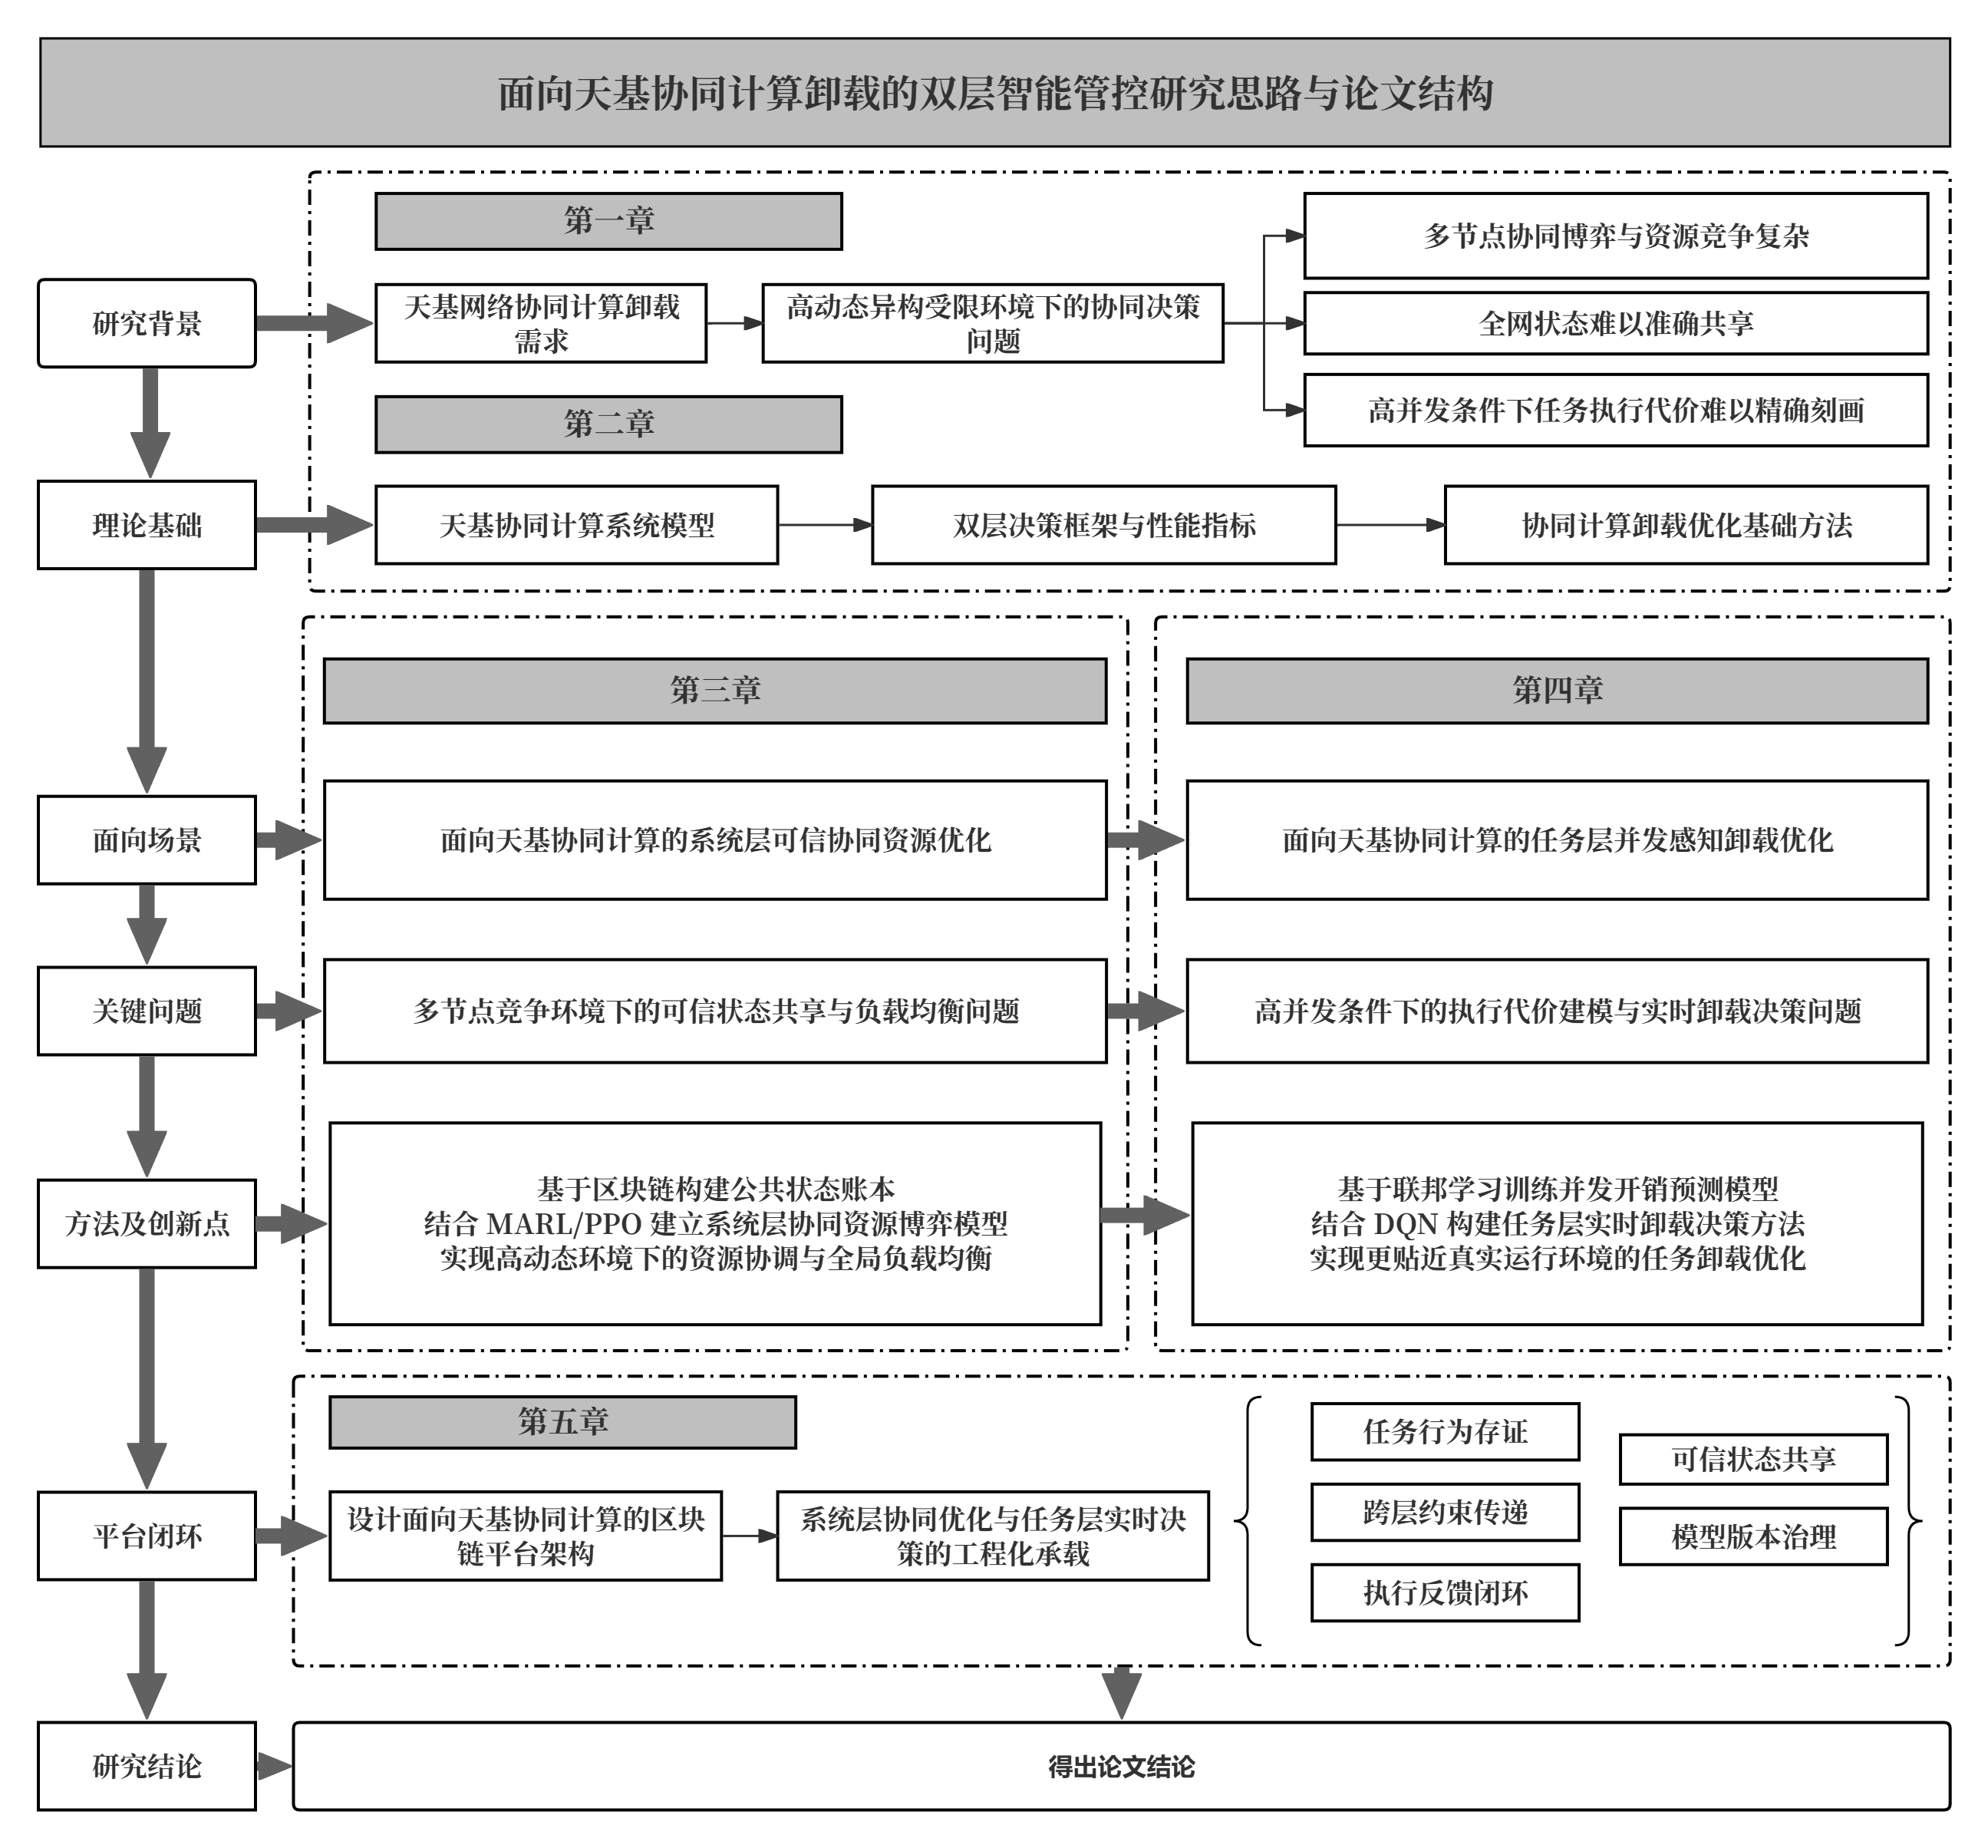
\includegraphics[width=0.85\textwidth]{figures/1-3.png}
  \caption{本论文研究思路及文章结构}
  \label{fig:structure}
\end{figure}

针对本文的研究工作，具体内容和章节安排如下：

第一章为绪论。首先介绍天基网络协同计算卸载的研究背景与意义，分析天基网络由传统转发网络向分布式协同计算平台演进的现实需求，以及在高动态、去中心化环境下面临的状态共享、资源协同、实时决策与平台承载等关键问题。其次，从天基边缘计算与任务卸载、动态环境下智能调度与多智能体协同、区块链协同与隐私保护学习三个方面，对国内外研究现状与发展趋势进行梳理。在此基础上，总结现有研究存在的主要问题与挑战，并给出本文的研究内容与整体结构安排。

第二章主要研究面向天基协同计算卸载的系统模型与理论基础。首先，结合卫星节点异构、链路时变、任务随机到达以及资源受限等特征，建立天基协同计算系统模型，形成对节点、任务、链路和资源约束的统一描述。其次，围绕系统层协同与任务层卸载所涉及的关键问题，梳理可信共享、多智能体协同、联邦学习和深度强化学习等相关理论基础，为后续章节的方法设计提供建模依据和理论支撑。

第三章研究基于区块链与MARL/PPO的系统层可信协同资源博弈方法。针对天基网络中全局状态难以准确获取、多节点之间易出现资源竞争与负载失衡的问题，构建面向系统层协同优化的可信状态共享与多智能体博弈框架。通过将区块链机制引入分布式状态维护过程，实现多节点资源信息的可信记录与共享；在此基础上，将多个卫星节点建模为多智能体，利用PPO策略优化实现系统层的协同资源调度与负载均衡。通过该章研究，为后续任务层卸载决策提供可信状态基础和系统协同环境。

第四章研究基于联邦学习与DQN的任务层并发感知卸载方法。针对传统卸载模型难以准确刻画多任务并发执行代价的问题，构建面向任务层实时决策的并发感知建模与智能卸载方法。首先，结合节点内部任务排队、资源争用和运行扰动等因素，建立更贴近真实运行环境的执行代价建模思路；其次，引入联邦学习机制，在保护各节点本地数据隐私的前提下完成并发代价预测模型训练；进一步结合DQN方法，将任务特征、链上状态和并发代价预测结果映射为具体卸载动作，实现面向动态环境的实时任务卸载优化。

第五章研究面向天基协同计算的区块链平台架构与运行机制。针对现有相关研究中算法设计与系统实现相互割裂的问题，在前述系统模型与双层智能方法基础上，设计能够统一承载可信共享、协同优化、模型治理与任务执行反馈的区块链平台架构。通过构建链上治理与链下计算相结合的运行机制，实现系统层与任务层方法的协同集成，为双层智能方法的工程化部署与可持续运行提供支撑。

第六章对全文工作进行总结，并对后续研究方向进行展望。
% !TeX root = ../main.tex
% =============================================================================
% 第 2 章 涉及的理论与技术基础（修订版）
% 修订要点：
% 1. 全章中文全角标点统一
% 2. 新增 §2.4 联邦学习与聚类联邦学习
% 3. 关键公式补充 \label{}，便于跨章引用
% 4. §2.5（原 §2.4）小节号顺延
% =============================================================================
\chapter{相关理论与技术基础}
\label{chap:ch2_background}

本章系统梳理本研究所涉及的天基网络计算卸载、区块链可信协同、联邦学习以及多智能体强化学习四类核心技术的基本原理、典型方法与应用边界，旨在为后续章节中天基协同计算系统的统一建模、长时间尺度协同优化以及短时间尺度卸载决策提供完整的理论支撑与技术依据。天基协同计算系统具有节点高速运动、链路时变、资源异构与可信环境受限等鲜明特征，传统地面边缘计算中所沿用的卸载方法与协同方法难以同时兼顾通信约束的精准刻画与协同决策的可信执行。本章梳理的四类前沿技术，正是本研究实现天基场景下高效卸载与可信协同的核心技术基础。

% -----------------------------------------------------------------------------
\section{天基网络与计算卸载技术}
\label{sec:ch2_satellite_offloading}

天基网络是指以低轨（Low Earth Orbit，LEO）、中轨（Medium Earth Orbit，MEO）和高轨（Geostationary Earth Orbit，GEO）卫星星座为核心，辅以地面控制中心、信关站及用户终端构成的一类天地一体化通信与计算网络。近年来，随着 LEO 巨型星座的快速部署与星上计算能力的持续提升，天基网络已从单纯的“通信中继”角色逐步演化为面向 6G 的“通信—感知—计算”一体化基础设施\cite{He2021,Wu2024ISL,Wang2024NTN,Saad2024NTNRel1718,Mahboob2024AINTN,Wang2025NTN6G}。本节将依次梳理天基网络的层级架构与链路特性、计算卸载的基本范式以及面向 LEO 环境的卸载决策方法。

\subsection{天基网络的层级架构与链路特性}
\label{subsec:ch2_sagin_arch}

目前关于天基网络的体系结构尚无统一规范，学术界普遍采用空—天—地一体化网络（Space–Air–Ground Integrated Network，SAGIN）的层级框架对其进行描述\cite{Wu2024ISL,LMCECN2025,Huang2024ICNLSMC}。在该框架下，LEO 卫星因其轨道低、传播时延小、链路增益高的优势，成为承载星上边缘计算的主要平台\cite{Sun2024MCO,Zhou2024MobilityAware}。本文将天基协同计算网络抽象为如下三层结构：

具体而言，用户终端层主要负责试验任务接入、任务属性提取和结果接收；星上边缘层由具备计算、缓存和星间通信能力的卫星边缘节点构成，承担任务本地处理、协同卸载和资源共享功能；地面控制层由地面控制中心和信关站等组成，主要负责系统管理、模型初始化、策略评估和长期运行维护。上述三层结构与第\ref{chap:ch3_unified_model}章中的 ST、SEN 和 CC 三类节点角色相对应。

天基网络的链路特性显著区别于地面网络，主要体现在三方面。第一，链路时变性强。LEO 卫星轨道周期约为90到100分钟，星—地、星—星之间的可见性窗口在分钟级尺度反复出现与消失，导致链路拓扑随时间剧烈变化\cite{Sun2024MCO}。第二，带宽与时延非对称。星—地下行链路普遍优于上行链路，且馈电链路与用户链路在频段、功率预算上差异显著\cite{Wang2024NTN}。第三，可达性受星历强约束，任意一对节点之间的端到端时延并非常数，而是随轨道相位的周期性变化的随机过程。上述特性使得传统假设链路恒定或缓变的卸载方法难以直接迁移，必须显式建模链路的时变性与可见性窗口约束。

本节梳理的天基网络层级结构是第\ref{chap:ch3_unified_model}章建模工作的应用背景。第\ref{chap:ch3_unified_model}章中将“用户终端层—星上边缘层—地面控制层”三层结构进一步形式化为卫星终端（Satellite Terminal，ST）、卫星边缘节点（Satellite Edge Node，SEN）和地面控制中心（Control Center，CC）三类节点角色，并在此基础上建立链路时延、可达性与资源异构的数学模型。

\subsection{计算卸载基本范式}
\label{subsec:ch2_offloading_paradigm}

计算卸载是指将计算密集型或时延敏感型任务从资源受限的终端节点迁移至算力充裕的边缘或云端节点执行的一类技术，其核心目标是在用户体验质量与系统资源开销之间取得平衡\cite{ref2,Tang2022DRL,Adu2026MADRL}。按卸载粒度划分，卸载方案通常包括二元卸载、部分卸载与依赖型卸载三类。二元卸载将任务视为不可分割的整体，决策变量仅为本地执行或卸载执行；部分卸载允许将任务按比例分割后并行处理；依赖型卸载则进一步考虑任务内部子模块之间的依赖关系，通常以有向无环图（Directed Acyclic Graph，DAG）的形式描述\cite{Guo2024E2E,Qu2024E2E}。

无论采用何种卸载粒度，卸载决策的形式化通常围绕时延、能耗与可靠性三项指标展开。任务在节点 $i$ 上的本地执行时延 $T^{\mathrm{loc}}_i$ 可表示为：
\begin{equation}
  T^{\mathrm{loc}}_i = \frac{c_k}{f_i}
  \label{eq:ch2_local_delay}
\end{equation}
其中 $c_k$ 为任务所需的 CPU 周期数，$f_i$ 为节点 $i$ 的计算频率。当任务被卸载至边缘节点 $j$ 时，端到端时延由传输时延、排队时延与边缘执行时延共同构成：
\begin{equation}
  T^{\mathrm{off}}_{i,j} = \frac{d_k}{r_{i,j}} + T^{\mathrm{queue}}_j + \frac{c_k}{f_j}
  \label{eq:ch2_offload_delay}
\end{equation}
其中 $d_k$ 为任务输入数据量，$r_{i,j}$ 为节点 $i$ 到节点 $j$ 的瞬时传输速率，$T^{\mathrm{queue}}_j$ 为目标节点的排队时延。能耗模型通常采用动态电压频率调整（Dynamic Voltage and Frequency Scaling，DVFS）假设，以芯片功耗系数 $\kappa$ 与计算频率立方的乘积形式表达\cite{Sun2024MCO}。

针对天基场景，计算卸载的研究焦点逐步从地面单跳卸载演进为多跳协同卸载与星—地联合卸载。Sun 等人\cite{Sun2024MCO}考虑 LEO 卫星运动性带来的链路时变，提出了运动感知的卸载策略，联合最小化网络时延与能耗。Wang 等人\cite{LMCECN2025}进一步将主从星协同纳入决策空间，提出多目标 D3QN 算法以兼顾任务完成率、负载均衡、时延与能耗。Guo 等人\cite{Guo2024E2E}则针对端到端任务，将卸载与路由联合建模为 NP 难问题并设计分解算法。近期面向对等卸载、服务部署、地星协同联邦学习和卫星边缘推理的研究进一步拓展了卸载决策的建模边界\cite{Zhang2024PeerOffloading,Tang2024TwoTimescaleJSAC,Zhai2024SECO,ref26,Fan2025SEI,Feng2026LatencyAware}。这些工作虽然在仿真层面验证了卸载在天基场景下的可行性，但普遍假设链路状态、节点信誉等关键变量集中可得，尚未充分考虑大规模、多管理域场景下“信息可信共享”这一前提。

本研究在第\ref{chap:ch3_unified_model}章定义的任务模型基础上，在第\ref{chap:ch5_task_offloading}章构建基于 DQN 的任务层卸载决策方法，并在此基础上引入由第\ref{chap:ch4_system_resource_allocation}章系统层下发的候选约束，以缓解上述工作中“集中可得信息”假设的局限。

\subsection{深度强化学习在卸载决策中的应用}
\label{subsec:ch2_drl_offloading}

由于卸载决策本质上是序列化决策问题，且环境状态具有高维、时变与部分可观特征，基于深度强化学习（Deep Reinforcement Learning，DRL）的方法近年来成为该领域的主流研究范式\cite{Mnih2015dqn,VanHasselt2016DoubleDQN,Wang2016Dueling,Tang2022DRL,Lim2022DRLOS}。DRL 通过将神经网络作为价值函数或策略函数的近似器，结合马尔可夫决策过程（Markov Decision Process，MDP）的形式化框架，实现对卸载策略的端到端学习。

深度 Q 网络（Deep Q-Network，DQN）是该领域的奠基性工作，其核心思想是用神经网络 $Q(s, a; \theta)$ 近似最优动作—价值函数，并通过经验回放和目标网络两项机制缓解训练发散问题\cite{Mnih2015dqn}。DQN 的更新目标为：
\begin{equation}
  y = r + \gamma \max_{a'} Q(s', a'; \theta^-)
  \label{eq:ch2_dqn_target}
\end{equation}
其中 $\theta^-$ 表示目标网络参数。然而原始 DQN 存在过估计偏差与价值估计与动作选择耦合两个问题。Double DQN 通过将动作选择与价值评估解耦缓解了过估计偏差，Dueling DQN 进一步将 Q 函数分解为状态价值与动作优势两支路，提升了在动作差异较小场景下的样本效率\cite{VanHasselt2016DoubleDQN,Wang2016Dueling,Lim2022DRLOS}：
\begin{equation}
  Q(s, a) = V(s) + A(s, a) - \frac{1}{|\mathcal{A}|}\sum_{a'} A(s, a')
  \label{eq:ch2_dueling}
\end{equation}

将 DQN 类方法应用于计算卸载场景的关键在于状态空间与动作空间的合理设计。Tang 与 Wong\cite{Tang2022DRL} 将节点队列状态、信道质量与历史决策共同纳入状态空间，采用 LSTM 与 Dueling DQN 结合的方式建模长期回报。Adu 等人\cite{Adu2026MADRL} 进一步在多接入边缘计算场景下将 DQN 扩展为多智能体形式，使每个边缘设备可基于本地观测做出去中心化卸载决策。Wang 等人\cite{LMCECN2025} 则针对 LEO 巨型星座设计了 D3QN 算法，在多目标（完成率、负载、时延、能耗）联合优化中取得了显著效果。

DQN 类方法是本研究第\ref{chap:ch5_task_offloading}章任务层方法的核心技术路径。第\ref{chap:ch5_task_offloading}章将以轻量化 DQN 为基础，以第\ref{chap:ch3_unified_model}章定义的链上摘要、链路状态与候选约束为状态输入，输出短时间尺度的离散卸载动作，并通过候选约束机制将系统层的协同意图传递到任务层执行。

% -----------------------------------------------------------------------------
\section{区块链与可信协同技术}
\label{sec:ch2_blockchain}

区块链是一种以链式数据结构存储交易、以分布式共识维护账本一致性、以密码学保证数据不可篡改的分布式账本技术\cite{ref3,ref13,ETSI2024BCFL,Villegas2025BETAC}。在天基协同计算场景下，引入区块链可在缺乏可信中心的条件下，为多管理域之间的状态共享、行为审计与模型治理提供透明、可追溯的可信底座\cite{ref12,ref15,ZhangLEO2024,Elmahallawy2025}。本节将分别介绍联盟链与共识机制、节点信誉机制，以及区块链辅助下的多方协同范式。

\subsection{联盟链与共识机制}
\label{subsec:ch2_consortium}

按节点准入策略划分，区块链可分为公有链、联盟链与私有链三类。公有链节点完全开放、采用工作量证明（Proof of Work，PoW）等高资源消耗共识，适合无中心化加密货币场景但难以适配资源受限的天基环境；私有链节点完全封闭、性能高但缺乏多方信任价值；联盟链则在两者之间取得平衡，通过组织级准入机制控制节点身份，采用拜占庭类共识保障一致性，既保留了分布式信任的优势，又显著降低了共识能耗，因而成为面向行业级可信协同的主流选择\cite{ETSI2024BCFL,NetTopoBFT2025}。

实用拜占庭容错（Practical Byzantine Fault Tolerance，PBFT）及其衍生算法是联盟链中最为广泛使用的共识机制。PBFT 通过预准备、准备、提交三阶段的多轮消息交互，在不超过 $\lfloor (n-1)/3 \rfloor$ 个拜占庭节点的前提下保证账本一致性，具有确定性最终性与无需挖矿的优势\cite{Lamport1982Byzantine,Castro1999,NetTopoBFT2025}。然而，经典 PBFT 算法的通信复杂度为
\begin{equation}
  \mathcal{C}_{\mathrm{PBFT}} = \mathcal{O}(n^2),
  \label{eq:ch2_pbft_complexity}
\end{equation}
在节点规模较大时延迟随节点数迅速恶化。为此，后续研究从两个方向加以改进：一是引入分片（Sharding）机制将共识负载分散到多个子链，显著提升系统吞吐\cite{ZhangLEO2024}；二是结合节点信誉对参与共识的节点子集进行动态筛选，将式~（\ref{eq:ch2_pbft_complexity}） 压缩为面向高信誉节点的 $\mathcal{O}(k^2)$ 通信（$k \ll n$），从而在大规模异构网络中保持可用的共识时延\cite{NetTopoBFT2025}。

智能合约（Smart Contract）是联盟链的核心可编程接口，其本质是部署在区块链上、由共识节点协同执行、执行结果上链可追溯的一段确定性代码。智能合约通过将业务逻辑显式表达为代码，使得多方协同中的关键判定（如准入审核、积分发放、违规惩戒）能够在无需可信第三方的条件下自动完成，极大提升了多方协同的执行效率与可审计性\cite{Androulaki2018Fabric,Villegas2025BETAC}。

本研究在第\ref{chap:ch3_unified_model}章中以联盟链作为天基协同计算系统的可信底座，将链上摘要、生命周期事件、节点信誉与模型版本等关键状态以分层共识方式维护；PBFT 类共识与智能合约则在第\ref{chap:ch4_system_resource_allocation}、\ref{chap:ch5_task_offloading}章方法中作为约束执行与凭据流转的实现假设。

\subsection{可信状态共享与节点信誉}
\label{subsec:ch2_reputation}

在多方协同的可信场景下，仅依靠共识机制保证账本一致性尚不足以支撑长期协作，还需进一步引入节点信誉（Reputation）机制对参与方的历史行为进行定量评估，以激励诚实行为、抑制恶意或低质量行为\cite{NetTopoBFT2025,ETSI2024BCFL}。节点信誉的核心在于将节点过往的行为（如任务执行准时率、模型更新质量、共识参与稳定性等）转换为一个随时间演化的可比较标量，并将该标量作为节点参与协同的权重或资格的判据。

典型的信誉演化模型采用指数加权移动平均的形式：
\begin{equation}
  R_i(t+1) = (1-\eta) R_i(t) + \eta r_i(t)
  \label{eq:ch2_reputation_update}
\end{equation}
其中 $R_i(t)$ 为节点 $i$ 在时刻 $t$ 的信誉值，$r_i(t)$ 为本轮的行为评分，$\eta$ 为学习率。信誉机制可与共识算法深度耦合，例如基于信誉的 PBFT 仅允许信誉高于阈值的节点参与共识投票，从而在保证安全的前提下进一步压缩共识规模\cite{NetTopoBFT2025}。

节点信誉机制是第\ref{chap:ch3_unified_model}章中“链上摘要—行为审计—权限调整”反馈环的关键中间变量，亦是第\ref{chap:ch4_system_resource_allocation}章系统层方法在筛选候选节点、第\ref{chap:ch5_task_offloading}章任务层方法在过滤目标节点时所共享的状态接口。式~（\ref{eq:ch2_reputation_update}） 是第\ref{chap:ch3_unified_model}章信誉更新规则的理论原型。

\subsection{区块链辅助的多方协同范式}
\label{subsec:ch2_bc_assisted}

区块链作为可信中介，已被广泛应用于多方协同场景下的去中心化数据共享、可追溯任务调度与多管理域治理。其典型应用范式包括：（1）将关键事件以哈希摘要的形式上链，原始数据保存于链下，形成“链上摘要 + 链下实体”的轻量化存证机制；（2）利用智能合约实现可编程的多方业务规则，例如自动化的资源分配、信誉惩戒和异常处置；（3）将分布式共识与多方协同决策深度耦合，使协同结果具备可审计性\cite{Feng2022,Moscato2023,ETSI2024BCFL,Elmahallawy2025}。

针对天基场景，Zhang 等人\cite{ZhangLEO2024} 提出了面向 LEO 网络的分片化区块链框架，通过将卫星节点按轨道平面划分为多个分片以缓解全网共识开销；Elmahallawy 等人\cite{Elmahallawy2025} 进一步将其拓展至多厂商星座场景，引入区块链辅助机制以应对跨星座间的信任薄弱问题。类似地，面向 LEO 卫星网络的分片化安全联邦学习框架也说明了共识负载拆分与模型更新存证之间的耦合价值\cite{ref29}。这些工作共同表明，区块链不仅是可信存储工具，还能与上层协同决策深度集成，构成多管理域天基协同的基础设施。

本研究将上述范式具体化为面向天基协同计算的“可信控制平面”：第\ref{chap:ch3_unified_model}章定义链上数据集合 $\mathcal{D}_{\mathrm{on}}$ 与摘要—对象哈希映射；第\ref{chap:ch4_system_resource_allocation}章利用链上公共摘要支撑系统层多智能体协同；第\ref{chap:ch5_task_offloading}章利用链上模型版本凭据支撑任务层并发开销预测模型的可信调用。

% -----------------------------------------------------------------------------
\section{联邦学习与聚类联邦学习}
\label{sec:ch2_federated_learning}

随着天基网络中的节点数量、任务多样性与隐私敏感性持续上升，传统的集中式机器学习范式难以满足“数据不出域”与“模型可协同”的双重要求。联邦学习（Federated Learning，FL）作为一类典型的隐私友好型分布式学习框架，能够在保留原始数据于本地的前提下，通过模型参数的多轮交换实现跨节点协同建模，已经成为天基边缘智能与跨星座协同的重要技术基础\cite{McMahan2017,Bonawitz2019,LiFedAvg2020,Li2020FederatedChallenges,Kairouz2021Advances}。本节首先介绍 FedAvg 算法及其在异质性条件下的局限，随后讨论聚类联邦学习的基本思想，最后回到区块链辅助的联邦学习范式与本研究的关联。

\subsection{FedAvg 算法与基本流程}
\label{subsec:ch2_fedavg}

FedAvg 是联邦学习领域最具代表性的基线算法。设全网共有 $N$ 个客户端，第 $k$ 个客户端的本地数据集为 $\mathcal{D}_k$，本地经验风险为 $F_k(w)$，则 FedAvg 的全局优化目标可写为
\begin{equation}
  \min_{w} f(w) = \sum_{k=1}^{N} p_k F_k(w),\qquad
  p_k = \frac{|\mathcal{D}_k|}{\sum_{j=1}^{N} |\mathcal{D}_j|},
  \label{eq:ch2_fedavg_objective}
\end{equation}
其中 $p_k$ 为客户端权重，通常正比于其本地样本量。FedAvg 的工作流程可概括为四步：（1）服务器初始化全局模型 $w^{(0)}$ 并下发至客户端；（2）每个客户端在本地以多轮 SGD 更新得到本地参数 $w_k^{(t+1)}$；（3）客户端将本地参数上传至服务器；（4）服务器按式~（\ref{eq:ch2_fedavg_objective}） 中的权重对客户端参数进行加权平均，得到新的全局模型
\begin{equation}
  w^{(t+1)} = \sum_{k=1}^{N} p_k\, w_k^{(t+1)}.
  \label{eq:ch2_fedavg_aggregation}
\end{equation}
在通信—聚合循环若干轮后，全局模型逐步收敛。FedAvg 的优势在于无需上传原始数据，仅交换模型参数，因而通信开销与隐私风险均较集中式训练显著下降\cite{McMahan2017,LiFedAvg2020}。

\subsection{数据异质性挑战与聚类联邦学习}
\label{subsec:ch2_clustered_fl}

然而，FedAvg 在面对客户端数据非独立同分布（Non-IID）时存在收敛慢、模型质量下降甚至训练发散的问题\cite{Li2020FedProx,Karimireddy2020Scaffold,Zou2024FL,FedFusion2024}。其根本原因在于：当不同客户端的本地最优解 $w_k^*$ 相差较大时，单一全局模型 $w$ 必然会落在某种“折中”位置，对多数客户端而言并非最优。在天基场景下，这一问题尤为突出——不同卫星节点的硬件能力、负载模式、任务类型与可见窗口差异显著，本地数据分布天然具有强异质性。

为缓解这一问题，聚类联邦学习（Clustered Federated Learning，Clustered FL）应运而生。其核心思想是放弃“全网共享单一模型”的强假设，转而将客户端按数据分布或参数更新方向划分为若干簇，每簇维护一个独立的簇模型，仅在簇内进行参数聚合。形式化地，设客户端被划分为 $K$ 个互不相交的簇 $\{\mathcal{C}_1, \mathcal{C}_2, \ldots, \mathcal{C}_K\}$，则第 $c$ 个簇在第 $t+1$ 轮的模型聚合可写为
\begin{equation}
  w_c^{(t+1)} = \sum_{k \in \mathcal{C}_c} \frac{|\mathcal{D}_k|}{\sum_{j \in \mathcal{C}_c} |\mathcal{D}_j|}\, w_k^{(t+1)}.
  \label{eq:ch2_clustered_fedavg}
\end{equation}
与式~（\ref{eq:ch2_fedavg_aggregation}） 相比，式~（\ref{eq:ch2_clustered_fedavg}） 的关键差异在于聚合范围被限制在“数据分布相近”的客户端子集内，从而能够保留局部模式、避免被全局平均效应淹没。簇划分本身可以基于客户端的负载特征、参数更新方向、梯度相似度或硬件能力等多种依据，常用方法包括 $k$-means 聚类、层次聚类与基于参数余弦相似度的动态分组\cite{sattler2021clusteredfl,Zou2024FL,FedFusion2024}。聚类联邦学习已在医疗影像、移动终端与物联网等多个异质性强的场景中表现出优于 FedAvg 的预测精度与收敛稳定性。

\subsection{区块链辅助的联邦学习}
\label{subsec:ch2_bcfl}

虽然联邦学习能够避免原始数据的集中传输，但其安全性仍依赖于一个可信的中心聚合服务器：一旦该服务器失效或被攻陷，恶意更新可能在不被察觉的情况下污染全局模型。区块链辅助的联邦学习（Blockchain-assisted Federated Learning，BCFL）将区块链作为可信聚合中介或可信凭据账本，将每轮的模型更新、参与方贡献、聚合凭据等以哈希摘要的形式上链，既消除了对中心聚合服务器的单点信任依赖，又借助区块链的可追溯性使恶意更新可被识别与回溯\cite{Feng2022,ETSI2024BCFL,Elmahallawy2025}。针对天基场景，Zhang 等人\cite{ZhangLEO2024}提出了面向 LEO 网络的分片化 BCFL 框架，通过将卫星节点按轨道平面划分为多个分片以缓解全网共识开销；Elmahallawy 等人\cite{Elmahallawy2025}进一步将其拓展至多厂商星座场景，引入 BCFL 以应对跨星座间的信任薄弱问题。面向地星融合网络的协同联邦学习研究也表明，局部计算、数据卸载与模型聚合需要联合设计\cite{ref26}。

本节梳理的 FedAvg、聚类联邦学习与 BCFL 是第\ref{chap:ch5_task_offloading}章任务层方法的核心技术路径之一。具体而言，第\ref{chap:ch5_task_offloading}章将基于式~（\ref{eq:ch2_clustered_fedavg}） 的簇内聚合规则训练并发开销预测模型，按节点并发任务数对节点进行分簇以应对工作负载的异质性；同时，将每轮聚合后的模型版本摘要按 BCFL 思想写入第\ref{chap:ch3_unified_model}章定义的模型版本集合 $\mathcal{D}^{\mathrm{model}}_{\mathrm{on}}$，实现“训练—发布—回滚”的可信治理闭环。

% -----------------------------------------------------------------------------
\section{多智能体强化学习与协同决策}
\label{sec:ch2_marl}

天基协同计算系统中，多个 SEN 节点需要在通信受限、信息部分可观的环境下做出长时间尺度的资源分配与候选筛选决策，其本质属于多智能体协同决策问题。与单智能体方法相比，多智能体强化学习（Multi-Agent Reinforcement Learning，MARL）需要同时应对环境非平稳性与动作空间指数级膨胀两大挑战\cite{Shapley1953,Lowe2017,Amato2024CTDE,Liu2025MARL}。本节将依次介绍 MARL 的基本框架、CTDE 训练范式以及代表性算法。

\subsection{多智能体马尔可夫决策过程}
\label{subsec:ch2_dec_pomdp}

多智能体协同决策问题通常形式化为去中心化部分可观马尔可夫决策过程（Decentralized Partially Observable Markov Decision Process，Dec-POMDP），其形式化定义为如下七元组：
\begin{equation}
  \langle \mathcal{N}, \mathcal{S}, \{\mathcal{A}_i\}_{i \in \mathcal{N}}, \mathcal{P},
  \mathcal{R}, \{\mathcal{O}_i\}_{i \in \mathcal{N}}, \gamma \rangle
  \label{eq:ch2_dec_pomdp}
\end{equation}
其中 $\mathcal{N}$ 为智能体集合，$\mathcal{S}$ 为全局状态空间，$\mathcal{A}_i$ 为智能体 $i$ 的动作空间，$\mathcal{P}$ 为状态转移函数，$\mathcal{R}$ 为团队共享奖励函数，$\mathcal{O}_i$ 为智能体 $i$ 的局部观测空间，$\gamma$ 为折扣因子。每个智能体 $i$ 仅可观测其局部观测 $o_i \in \mathcal{O}_i$，根据策略 $\pi_i(a_i \mid o_i)$ 选择动作，所有智能体共同最大化期望累积折扣奖励：
\begin{equation}
  J(\boldsymbol{\pi}) = \mathbb{E}_{\boldsymbol{\pi}}
  \!\left[\sum_{t=0}^{\infty} \gamma^t \mathcal{R}(s_t, \mathbf{a}_t)\right]
  \label{eq:ch2_marl_objective}
\end{equation}

Dec-POMDP 的核心难点在于，从任意单个智能体的角度看，其他智能体策略的演变会使得环境呈现非平稳特征（Non-stationarity），从而违反单智能体强化学习中环境动态平稳的关键假设\cite{Tsitsiklis1997,Liu2025MARL}。这种非平稳性是直接将单智能体方法独立部署于多智能体环境时，常常出现训练不稳定甚至发散的根本原因。

\subsection{集中训练分散执行范式}
\label{subsec:ch2_ctde}

集中训练分散执行（Centralized Training with Decentralized Execution，CTDE）是当前缓解 MARL 非平稳性问题的主流框架\cite{Amato2024CTDE}。CTDE 的核心思想是：在训练阶段，各智能体可访问全局状态或其他智能体的私有信息，从而在更准确的环境模型下学习策略；而在执行阶段，各智能体仅依据本地观测做出决策，从而满足现实通信受限场景的部署约束。CTDE 框架与全局集中式方法相比，显著缓解了动作空间随智能体数指数增长的扩展性问题；与全分散式方法相比，又通过训练阶段的全局信息共享避免了非平稳性带来的训练失稳。

CTDE 范式下的代表性算法可分为价值分解（Value Decomposition）与集中评论家（Centralized Critic）两大类。价值分解方法将团队联合 $Q$ 函数分解为各智能体局部 $Q$ 函数的某种聚合，代表性工作包括 VDN、QMIX 与 QPLEX，其单调性约束保证了局部最优与全局最优的一致性\cite{Sunehag2018VDN,Rashid2018QMIX,Amato2024CTDE}。集中评论家方法则在训练时维护一个以全局状态为输入的中心化评论家网络，并以此指导各智能体局部策略的更新，代表性工作包括 MADDPG 与 MAPPO\cite{Lowe2017,ref5,Liu2025MARL}。

MAPPO 作为近年来最受关注的 CTDE 算法之一，将单智能体 PPO 扩展到多智能体场景，通过共享参数与集中评论家显著提升训练稳定性。其策略更新目标为：
\begin{equation}
  L^{\mathrm{CLIP}}(\theta) = \mathbb{E}\!\left[
    \min\!\Big(\rho_t(\theta) \hat{A}_t,
    \mathrm{clip}(\rho_t(\theta), 1-\epsilon, 1+\epsilon) \hat{A}_t\Big)
    \right]
  \label{eq:ch2_ppo_clip}
\end{equation}
其中 $\rho_t(\theta) = \pi_\theta(a_t \mid o_t) / \pi_{\theta_{\mathrm{old}}}(a_t \mid o_t)$ 为重要性比率，$\hat{A}_t$ 为基于集中评论家估计的优势函数，$\epsilon$ 为裁剪系数。MAPPO 在 SMAC、GRF 等基准上的表现已被多项研究证实其综合性能优于 QMIX 等价值分解方法\cite{ref5}。

\subsection{协同决策中的奖励设计与扩展性}
\label{subsec:ch2_marl_reward}

奖励函数设计是 MARL 应用于具体协同问题的关键环节。共享团队奖励能够在原则上鼓励合作，但在大规模智能体场景下会引发信用分配（Credit Assignment）问题——即难以从团队整体奖励中区分各个智能体的具体贡献。COMA 等反事实基线方法通过构造“假设智能体 $i$ 执行其他动作”的对照基线，显式估计每个智能体对团队奖励的边际贡献，从而缓解信用分配难题\cite{ref11,Amato2024CTDE}。在工程实践中，常用方法是将团队奖励与个体奖励按比例加权，从而在协同性与个体可控性之间寻求平衡。

针对扩展性问题，近期研究探索了基于图神经网络的层级注意力机制\cite{Li2024MARL_GA}，通过对智能体之间的依赖关系建模，将注意力计算压缩到必要的邻居子集，从而显著降低智能体规模带来的状态拼接维度。该思路与本研究中“基于信誉与可见性筛选候选邻居”的协同模式具有较强的契合性。

CTDE 范式与 MAPPO 算法是本研究第\ref{chap:ch4_system_resource_allocation}章系统层方法的核心技术路径。第\ref{chap:ch4_system_resource_allocation}章将以每个 SEN 抽象为一个智能体，以第\ref{chap:ch3_unified_model}章定义的链上共享状态作为观测输入，通过 MAPPO 联合学习任务流向偏好、资源分配比例和外部任务接收意愿等长时间尺度协同动作，并通过候选约束机制将协同意图下发至第\ref{chap:ch5_task_offloading}章的任务层执行。式~（\ref{eq:ch2_ppo_clip}） 即为第\ref{chap:ch4_system_resource_allocation}章策略更新目标的理论原型。

% -----------------------------------------------------------------------------
% -----------------------------------------------------------------------------
\section{本章小结}
\label{sec:ch2_summary}

本章围绕本文后续方法设计所需的理论基础，分别介绍了天基网络与计算卸载、区块链可信协同、联邦学习与聚类联邦学习、多智能体强化学习等相关技术。在天基网络与计算卸载方面，本章梳理了天基网络的层级结构、链路时变特性以及卸载决策的基本时延模型，为第\ref{chap:ch3_unified_model}章构建卫星终端、卫星边缘节点、地面控制中心和动态链路模型提供基础。在区块链可信协同方面，本章介绍了联盟链、共识机制、智能合约和节点信誉机制，为后续可信状态共享、行为审计和链上反馈机制提供支撑。在联邦学习与聚类联邦学习方面，本章说明了分布式数据不出域条件下的模型协同训练方法，为第\ref{chap:ch5_task_offloading}章并发开销预测模型的训练提供理论依据。在多智能体强化学习方面，本章介绍了Dec-POMDP、CTDE和MAPPO等基本方法，为第\ref{chap:ch4_system_resource_allocation}章多节点系统层协同资源分配奠定基础。

总体而言，本章的作用在于为后续章节提供必要的理论和技术支撑，后续第\ref{chap:ch3_unified_model}章将在上述技术基础上建立天基协同计算卸载统一模型；第\ref{chap:ch4_system_resource_allocation}章将结合区块链可信状态共享与多智能体强化学习，研究系统层协同资源分配方法；第\ref{chap:ch5_task_offloading}章将结合聚类联邦学习与DQN，研究并发开销感知的任务层实时卸载方法。由此，本文形成从理论基础到统一建模，再到系统层协同和任务层卸载的递进关系。

%%
% 第三章 天基网络可信协同计算卸载场景与基础建模
%%

\chapter{天基网络可信协同计算卸载场景与基础建模}
\label{chap:ch3_unified_model}

\section{引言}
\label{sec:ch3_intro}

天基网络协同计算卸载的主要挑战不仅仅是技术优化，而是如何应对动态拓扑、异构资源与可信协同之间的复杂约束。卫星轨道的运动使得星间与星地链路的可达性、带宽以及可见窗口不断变化，网络拓扑表现出强烈的时变特性。此外，卫星终端、卫星边缘节点以及地面控制中心在计算能力、存储容量、能量预算和通信条件上存在显著差异，无法采用静态的集中式调度模型。

协同卸载是一个由多个节点参与的分布式过程，网络中缺乏稳定且持续可达的中心节点，节点状态上报存在延迟、失真甚至虚假报告的问题，任务执行的结果和协同行为需要具备可信的追溯机制。因此，天基网络协同计算卸载不仅要解决资源匹配和任务分配，还需要在拓扑动态性、资源异构性和状态可信性之间建立统一的建模框架。

目前，已有研究多从单一角度处理上述问题。计算卸载相关研究通常采用简化的节点与链路假设，重点关注时延与能耗优化，对节点状态可信共享、任务执行追溯以及长期协作激励考虑不足；面向多时间尺度的研究则往往分别讨论系统层长期协同与任务层即时决策，尚未充分刻画二者在同一方法体系中的层次衔接关系。若协同资源分配、可信状态共享与任务卸载决策分别采用彼此独立的符号体系和建模假设，则系统层协同结果难以自然转化为任务层约束，任务层执行反馈也难以回流至系统层状态更新。因此，在具体方法展开之前，有必要建立涵盖网络拓扑、节点资源、任务属性、链路传输、执行代价以及区块链可信控制平面结构和状态摘要的统一基础模型，为后续章节的状态构造、代价计算与目标函数设计奠定一致的形式化基础。

为此，本章在第\ref{chap:ch4_system_resource_allocation}章和第\ref{chap:ch5_task_offloading}章的具体方法设计之前，首先给出统一的天基网络协同计算卸载场景描述与基础建模。具体来说，本章的目标有两方面：一方面，描绘由卫星终端、卫星边缘节点、地面控制中心和区块链可信控制平面共同组成的协同计算卸载场景，明确参与角色、任务生命周期流程与基本运行框架；另一方面，建立一个统一的符号体系，涵盖网络拓扑、节点资源、任务属性、链路传输、本地计算、星间卸载、能耗开销、联盟链结构与链上状态摘要等基础模型，为后续章节中的代价计算、状态构造与目标函数设计提供共同的形式化基础。

\section{天基网络可信协同计算卸载场景}
\label{sec:ch3_scenario}
\label{subsec:ch3_blockchain_role}

本节首先给出本文所研究的协同计算卸载场景。整个场景由物理网络层和区块链可信控制平面共同支撑：物理网络层提供节点之间动态时变的星间与星地链路，是任务执行与数据传输的物理载体；区块链可信控制平面以联盟链与智能合约为载体，承载节点状态摘要、任务生命周期事件、节点信誉演化与模型版本凭据等可信公共信息。参与协同计算的实体进一步划分为卫星终端、卫星边缘节点、地面控制中心和区块链可信控制平面四类角色，并在其上协同完成由``任务生成—状态感知—候选节点筛选—卸载决策—任务执行—结果反馈—链上更新''七个阶段构成的任务生命周期流程。场景的总体结构如图\ref{fig:ch3_scenario_overview}所示。

\begin{figure}[htbp]
    \centering
    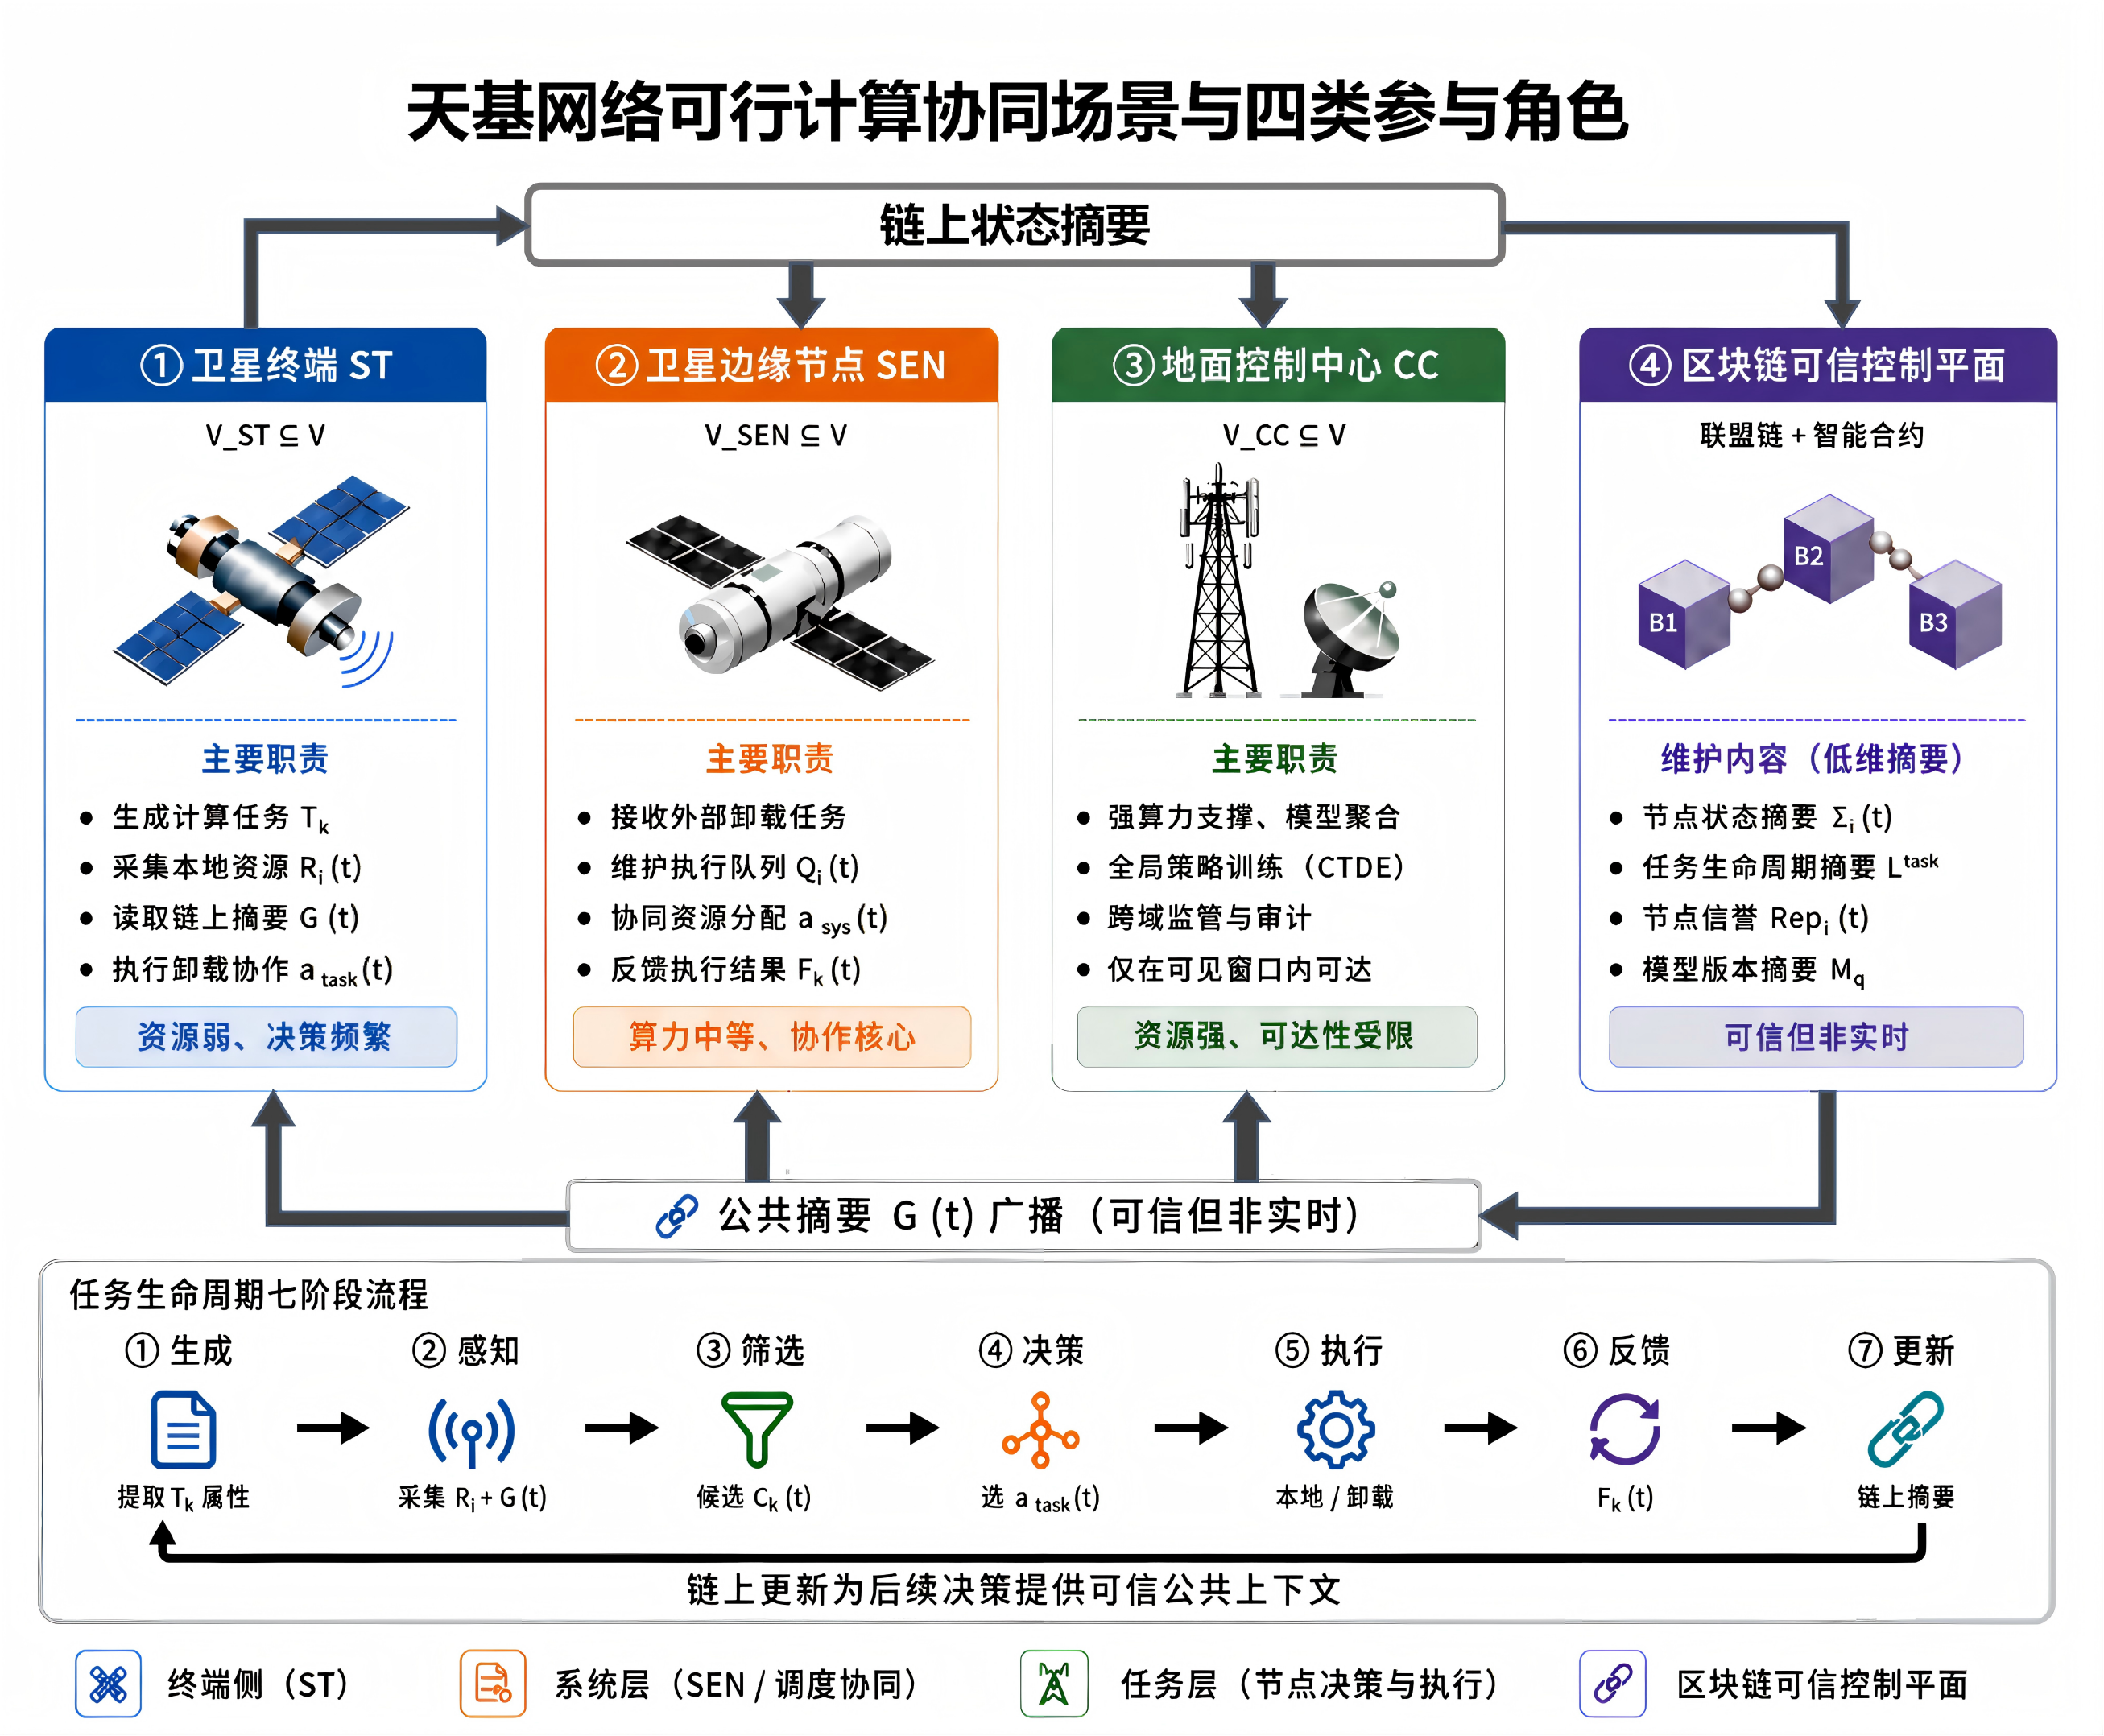
\includegraphics[width=0.96\textwidth]{figures/new3-2.png}
    \caption{天基网络可信协同计算卸载场景与四类参与角色}
    \label{fig:ch3_scenario_overview}
\end{figure}

图\ref{fig:ch3_scenario_overview}从上至下展示了天基网络可信协同计算卸载场景的三类要素：物理网络层、四类参与角色与任务生命周期流程。

物理网络层刻画卫星轨道运动以及由此产生的时变星间和星地链路。链路的可达性、可用带宽和可见窗口随轨道相对几何关系动态变化，使节点之间的状态广播频率和传输能力同样具有时变特性。节点本地状态摘要 $\Sigma_i(t)$ 在频次受控的前提下经此层链路上链，其上链频率综合考虑链路带宽预算、可见窗口长度和共识开销三方面约束，避免因高频上链而挤占任务数据通信带宽；具体的网络拓扑模型与链路状态向量将在第\ref{subsec:ch3_topology_model}节形式化给出。

天基网络可信协同计算卸载场景主要有四类参与角色，分别承担不同的协同职责。卫星终端 ST（属于 $\mathcal{V}_{\mathrm{ST}}$）一般指资源受限的小型卫星或专用终端，其特点是计算与能量资源相对薄弱、决策频繁，主要负责生成计算任务、采集本地资源状态、读取链上公共摘要并执行卸载动作，是任务发起方；卫星边缘节点 SEN（属于 $\mathcal{V}_{\mathrm{SEN}}$）通常为具备较强算力与转发能力的卫星平台，是协作执行的核心，负责接收外部卸载任务、维护执行队列、参与协同资源分配并向链上反馈执行结果；地面控制中心 CC（属于 $\mathcal{V}_{\mathrm{CC}}$）资源最为充裕，但其与天基节点之间的可达性受限于轨道可见窗口，主要承担强算力支持、模型聚合、全局策略训练以及跨域监管与审计等职责；区块链可信控制平面以联盟链与智能合约为载体，本身不直接参与高频任务执行，而是作为可信状态共享与治理底座，维护节点状态摘要、任务生命周期事件、节点信誉评分与模型版本摘要等低维可信信息，并通过公共摘要向前三类角色统一广播。

形式化地，参与协同计算的节点集合可表示为
\begin{equation}
    \mathcal{V}=\mathcal{V}_{\mathrm{ST}}\cup\mathcal{V}_{\mathrm{SEN}}\cup\mathcal{V}_{\mathrm{CC}}.
    \label{eq:ch3_node_set}
\end{equation}
任一物理节点既可能是任务发起方，也可能是任务执行方，但不同节点在算力、存储、能量和链路条件上存在显著差异。为支撑后续可信状态共享建模，本文进一步从功能职责角度定义共识维护节点集合 $\mathcal{V}_{\mathrm{con}}\subseteq\mathcal{V}$、任务执行节点集合 $\mathcal{V}_{\mathrm{exe}}\subseteq\mathcal{V}$ 和链下存储节点集合 $\mathcal{V}_{\mathrm{sto}}\subseteq\mathcal{V}$。三类集合分别对应区块定序与状态摘要广播、任务承接与执行反馈、以及大规模实体对象的链下存储。需要说明的是，这里的 $\mathcal{V}_{\mathrm{exe}}$ 表示物理意义上的任务执行能力集合，并不等同于联盟链网络中的非共识账本节点；同一物理节点可同时承担多种功能职责，例如核心 SEN 可同时参与共识和任务执行，CC 在可见窗口内也可兼具共识、执行和链下存储能力。因此，$\mathcal{V}_{\mathrm{con}}$、$\mathcal{V}_{\mathrm{exe}}$ 与 $\mathcal{V}_{\mathrm{sto}}$ 之间允许存在交集。

任务生命周期七阶段流程刻画了一次具体协同计算从发起到完成所经历的关键阶段。生成：卫星终端产生计算任务并提取 $T_k=(s_k,c_k,d_k,\tau_k,\zeta_k,t_k^{\mathrm{arr}})$ 等任务属性；感知：终端采集本地资源状态 $R_i(t)$ 与链上公共摘要 $G(t)$，形成``本地观测+链上摘要''的复合状态视图；筛选：基于链路可见窗口、节点信誉门限与负载约束确定可卸载候选节点集合 $\mathcal{N}_k^{\mathrm{off}}(t)$，并与本地节点共同构成任务动作集合 $\mathcal{A}_k(t)$；决策：在 $\mathcal{A}_k(t)$ 上根据时延、能耗与并发开销估计选择本地执行或卸载动作 $a_{\mathrm{task}}(t)$；执行：目标节点（本地或卸载节点）完成任务计算与结果回传；反馈：系统记录任务完成时延、能耗、成功状态和异常事件，封装为反馈向量 $F_k(t)$；更新：反馈摘要写入链上，进而更新节点信誉、负载摘要与模型版本统计，并以``链上更新驱动下一轮决策''的方式形成持续演化。

由上述阶段可见，协同计算卸载并不是简单的``任务发起—节点选择—执行返回''的单向调用，而是由感知、决策、执行、反馈和更新共同支撑的持续过程：状态感知与链上更新提供可信公共上下文，候选节点筛选与卸载决策由后续章节中的系统层和任务层方法分别承担，任务执行结果则通过链上事件回流为后续策略迭代提供依据。关于该过程在不同时间尺度下的形式化描述以及两层方法之间的耦合机制，将在第\ref{chap:ch4_system_resource_allocation}章和第\ref{chap:ch5_task_offloading}章中分别给出。

图\ref{fig:ch3_scenario_overview}最右侧的区块链可信控制平面被本文定位为``可信但非实时''的状态共享与治理底座。这一定位包含两层含义。其一，该控制平面不直接替代实时调度器，亦不存储高维原始任务数据，而是仅维护协同所需的低维可信信息：通过摘要上链与实体链下存储相结合的方式，为系统层协同资源分配提供可信公共状态、为任务层卸载决策提供候选节点摘要与模型版本凭据，并通过任务执行结果回流更新节点信誉与系统状态；具体的联盟链网络组成、区块结构以及链上状态摘要的形式化定义将在第\ref{subsec:ch3_chain_structure}节与第\ref{subsec:ch3_state_summary}节给出，而节点信誉演化、任务生命周期存证和模型版本可信维护等动态治理机制由于与下游方法的状态空间和奖励设计紧密耦合，将在第\ref{chap:ch4_system_resource_allocation}章和第\ref{chap:ch5_task_offloading}章中分别展开。其二，``非实时''是指区块链共识、广播与验证的总附加时延 $D_{\mathrm{chain}}$ 通常处于亚秒至数秒量级。由于系统层多节点资源协同关注较长时间尺度上的负载演化与信誉积累，而任务层卸载决策受任务到达瞬间的链路窗口与队列状态约束，$D_{\mathrm{chain}}$ 在系统层尺度上可被视为可容忍的小量，但在任务层尺度上不可忽略。具体的时间尺度划分以及链上摘要在不同方法中的嵌入方式，将在第\ref{chap:ch4_system_resource_allocation}章和第\ref{chap:ch5_task_offloading}章中结合各自方法的决策粒度分别给出。

\section{系统基础模型}
\label{sec:ch3_basic_model}

本节按照``物理资源—任务与代价—可信控制''的逻辑展开，建立后续章节共用的符号体系。其中，第\ref{subsec:ch3_topology_model}节至第\ref{subsec:ch3_exec_model}节刻画 ST/SEN/CC 三类计算节点的物理属性与执行代价，第\ref{subsec:ch3_chain_structure}节至第\ref{subsec:ch3_state_summary}节刻画区块链可信控制平面的结构组成与状态摘要。各子模型在完成形式化定义后，进一步说明其与系统层协同资源分配和任务层实时卸载决策之间的层次关系，以保证全文建模假设、变量含义和方法展开的一致性。

\subsection{网络拓扑模型}
\label{subsec:ch3_topology_model}

天基网络拓扑随轨道运动和链路可见关系动态变化。本文将其表示为时变有向图
\begin{equation}
    \mathcal{G}(t)=\big(\mathcal{V},\mathcal{E}_{\mathrm{link}}(t)\big),
    \label{eq:ch3_dynamic_graph}
\end{equation}
其中，$\mathcal{V}$ 由式\eqref{eq:ch3_node_set}给出，$\mathcal{E}_{\mathrm{link}}(t)$ 为时刻 $t$ 可用通信链路集合。若节点 $i$ 与节点 $j$ 在时刻 $t$ 存在可用链路，则 $(i,j)\in\mathcal{E}_{\mathrm{link}}(t)$。链路状态可表示为
\begin{equation}
    \ell_{ij}(t)=\big(B_{ij}(t),d_{ij}^{\mathrm{prop}}(t),\tau_{ij}^{\mathrm{vis}}(t),p_{ij}^{\mathrm{loss}}(t)\big),
    \label{eq:ch3_link_state}
\end{equation}
其中，$B_{ij}(t)$ 为可用带宽，$d_{ij}^{\mathrm{prop}}(t)$ 为传播时延，$\tau_{ij}^{\mathrm{vis}}(t)$ 为剩余可见窗口，$p_{ij}^{\mathrm{loss}}(t)$ 为链路中断概率估计。

上述拓扑与链路状态定义给出了节点间协同关系的物理可行域。在系统层协同资源分配中，$\ell_{ij}(t)$ 可被进一步聚合为链路统计特征，用以刻画节点之间长期协作的稳定性与可达性；在任务层实时卸载决策中，$\tau_{ij}^{\mathrm{vis}}(t)$ 则构成候选节点筛选的重要约束，决定当前任务是否能够在链路可见窗口内完成传输与返回。

\subsection{节点资源模型}
\label{subsec:ch3_resource_model}

节点 $v_i$ 的资源状态定义为
\begin{equation}
    R_i(t)=\big(F_i(t),M_i(t),Q_i(t),E_i(t),\rho_i(t),\mathrm{Rep}_i(t)\big),
    \label{eq:ch3_resource_state}
\end{equation}
其中，$F_i(t)$ 表示可用计算能力，$M_i(t)$ 表示可用存储或缓存容量，$Q_i(t)$ 表示任务队列长度，$E_i(t)$ 表示剩余能量或能量预算，$\rho_i(t)$ 表示资源利用率，$\mathrm{Rep}_i(t)$ 表示节点信誉评分。资源状态在每个决策周期由节点本地采样获得，再经摘要化处理后上链共享，其摘要形式将在第\ref{subsec:ch3_state_summary}节给出；信誉评分 $\mathrm{Rep}_i(t)$ 的具体演化规则将在第\ref{chap:ch4_system_resource_allocation}章第\ref{subsec:ch4_reward_design}节中结合系统层奖励函数设计给出。

基于上述资源状态表示，后续章节可在不同时间尺度下选取相应状态分量。第\ref{chap:ch4_system_resource_allocation}章面向窗口级协同，将 $R_i(t)$ 投影为节点局部观测 $l_t^i$，以刻画节点长期负载与协作能力；第\ref{chap:ch5_task_offloading}章面向单任务到达瞬间的实时决策，则从中抽取队列长度、剩余能量和资源利用率等局部状态，形成任务层状态 $\bm{x}^{\mathrm{local}}$。

\subsection{任务模型}
\label{subsec:ch3_task_model}

设任务集合为 $\mathcal{T}$。任一任务 $T_k$ 可表示为
\begin{equation}
    T_k=\big(s_k,c_k,d_k,\tau_k,\zeta_k,t_k^{\mathrm{arr}}\big),
    \label{eq:ch3_task_model}
\end{equation}
其中，$s_k$ 为任务输入数据规模，$c_k$ 为完成任务所需的 CPU 周期数，$d_k$ 为任务最大可接受完成时延，$\tau_k$ 为任务类型标识，$\zeta_k$ 为任务优先级，$t_k^{\mathrm{arr}}$ 为任务到达时间。该表示方式既适用于遥感图像识别、目标检测等智能推理任务，也适用于通信解调、数据压缩和信号处理等传统计算任务。后文所有与链路可见窗口有关的约束均采用时延量 $D_{k,ij}^{\mathrm{tx}}(t)$ 或任务截止时延 $d_k$ 表示，$\tau_k$ 仅作为任务类型标识使用。

为使建模具有典型物理锚点，本文以低轨遥感星座辅助应急图像识别任务作为参考场景：考虑由若干卫星终端、卫星边缘节点和地面控制中心构成的协同计算网络，单次试验典型时长为分钟级，单任务典型输入数据规模为兆字节量级，典型计算量为百万至十亿浮点运算量级。第\ref{chap:ch4_system_resource_allocation}章和第\ref{chap:ch5_task_offloading}章的实验将分别在该场景下，按照系统层和任务层不同时间尺度展开。

在后续两章中，任务模型对应不同粒度的状态刻画。第\ref{chap:ch4_system_resource_allocation}章关注统计窗口内任务负载的整体演化，因此将 $\mathcal{T}$ 中任务类型、计算量和截止期等信息聚合为任务分布摘要 $D^{\mathrm{task}}(t)$；第\ref{chap:ch5_task_offloading}章关注单任务到达时的即时动作选择，因此将 $T_k$ 的输入规模、计算量、时延约束、任务类型和优先级组织为任务特征向量 $\bm{x}^{\mathrm{task}}$。

\subsection{链路传输模型}
\label{subsec:ch3_tx_model}

当任务 $T_k$ 从节点 $i$ 卸载至节点 $j$ 时，其传输速率可写为
\begin{equation}
    R_{ij}(t)=B_{ij}(t)\log_2\!\left(1+\frac{P_i h_{ij}(t)}{N_0 B_{ij}(t)}\right),
    \label{eq:ch3_rate_model}
\end{equation}
其中，$P_i$ 为节点 $i$ 的发送功率，$h_{ij}(t)$ 为信道增益，$N_0$ 为噪声功率谱密度。相应传输时延为
\begin{equation}
    D_{k,ij}^{\mathrm{tx}}(t)=\frac{s_k}{R_{ij}(t)}+d_{ij}^{\mathrm{prop}}(t).
    \label{eq:ch3_tx_delay}
\end{equation}

式\eqref{eq:ch3_rate_model}和式\eqref{eq:ch3_tx_delay}刻画了任务跨节点传输的基本时延构成。第\ref{chap:ch5_task_offloading}章将在任务层采用 $L_i^{\mathrm{off}}(n,t)$ 表示卸载至候选节点 $n$ 时的端到端完成时延，其中上行传输时延由式\eqref{eq:ch3_tx_delay}给出。为区分基础链路时延与任务层端到端时延，本文在本章采用 $D$ 表示基础时延量，在第\ref{chap:ch5_task_offloading}章采用 $L$ 表示任务完成时延，两者在物理含义上相互一致，在建模粒度上有所区别。

\subsection{本地计算与星间卸载模型}
\label{subsec:ch3_exec_model}

若任务在本地执行，其完成时延为
\begin{equation}
    D_{k,i}^{\mathrm{loc}}(t)=W_i(t)+\frac{c_k}{f_{k,i}^{\mathrm{alloc}}(t)},
    \label{eq:ch3_local_compute_delay}
\end{equation}
其中，$W_i(t)$ 为排队等待时延，$f_{k,i}^{\mathrm{alloc}}(t)$ 为节点 $i$ 分配给任务 $T_k$ 的有效计算频率。若任务卸载至节点 $j$ 执行，其完成时延为
\begin{equation}
    D_{k,ij}^{\mathrm{off}}(t)=D_{k,ij}^{\mathrm{tx}}(t)+W_j(t)+\frac{c_k}{f_{k,j}^{\mathrm{alloc}}(t)}+\Delta_{k,j}^{\mathrm{conc}}(t),
    \label{eq:ch3_offload_delay_unified}
\end{equation}
其中，$\Delta_{k,j}^{\mathrm{conc}}(t)$ 表示多任务并发引起的额外开销，既包括新任务自身完成时延的增加，也包括新任务加入后对目标节点存量任务剩余完成时间的影响。该项体现了任务层卸载决策中资源竞争与任务耦合的关键因素，第\ref{chap:ch5_task_offloading}章将进一步对其进行形式化分解与近似刻画。为减少符号负担，第\ref{chap:ch5_task_offloading}章在单任务视角下将 $\Delta_{k,j}^{\mathrm{conc}}(t)$ 记为 $\Delta_i(n,t)$，其中 $i$ 表示新到达任务，$n$ 表示候选目标节点；并将其完整形式化定义记为 $CO_i(n,t)$，预测估计记为 $\widehat{\Delta}_i(n,t)$，各分量含义均与本章保持一致。

本地执行能耗可近似表示为
\begin{equation}
    E_{k,i}^{\mathrm{loc}}(t)=\kappa_i c_k\big(f_{k,i}^{\mathrm{alloc}}(t)\big)^2,
    \label{eq:ch3_local_energy_unified}
\end{equation}
其中，$\kappa_i$ 为节点 $i$ 的有效电容系数。卸载执行能耗可表示为
\begin{equation}
    E_{k,ij}^{\mathrm{off}}(t)=P_i \frac{s_k}{R_{ij}(t)}+\kappa_j c_k\big(f_{k,j}^{\mathrm{alloc}}(t)\big)^2+E_{k,ij}^{\mathrm{wait}}(t),
    \label{eq:ch3_offload_energy_unified}
\end{equation}
其中，$E_{k,ij}^{\mathrm{wait}}(t)$ 表示等待和连接维持过程中的额外能耗。

上述本地执行与卸载执行模型构成全文统一的代价刻画基础。第\ref{chap:ch4_system_resource_allocation}章将在统计窗口内聚合相应时延与能耗项，以形成系统层奖励函数中的效率评价；第\ref{chap:ch5_task_offloading}章则在单任务粒度上进一步展开等待能耗、边缘侧执行能耗折算和并发扰动项，并据此构造任务层综合代价 $J_i(a_t)$。因此，后续章节中能耗项的具体展开可理解为对本章基础代价模型的时间尺度细化，而非另行引入新的物理代价假设。

\subsection{联盟链结构与区块结构}
\label{subsec:ch3_chain_structure}

考虑到天基协同计算环境中节点身份相对受控、共识效率约束严格、不同业务事件之间存在频次与时效差异，本文采用联盟链方式组织区块链可信控制平面，并对其网络结构、链上链下数据划分以及区块结构进行形式化描述。本小节给出联盟链的结构性定义，而具体的事件写入、共识流程以及节点信誉演化、任务生命周期存证、模型版本治理等动态机制将在下游章节结合方法流程展开。

\subsubsection{联盟链网络组成}

设区块链网络由一组授权账本节点 $\mathcal{V}_{\mathrm{chain}}\subseteq\mathcal{V}$ 构成。按照账本维护权限，可将其划分为共识节点集合 $\mathcal{V}_{\mathrm{con}}$ 和账本接入节点集合 $\mathcal{V}_{\mathrm{cli}}$。其中，$\mathcal{V}_{\mathrm{con}}$ 负责区块定序、交易校验与状态广播，是账本一致性的直接维护方；$\mathcal{V}_{\mathrm{cli}}$ 不参与区块生成，但可进行状态读取、事件提交与本地校验。二者满足 $\mathcal{V}_{\mathrm{con}}\cap\mathcal{V}_{\mathrm{cli}}=\varnothing$ 且 $\mathcal{V}_{\mathrm{con}}\cup\mathcal{V}_{\mathrm{cli}}=\mathcal{V}_{\mathrm{chain}}$。需要强调的是，$\mathcal{V}_{\mathrm{cli}}$ 仅表示联盟链中的账本访问身份，与前文定义的任务执行节点集合 $\mathcal{V}_{\mathrm{exe}}$ 属于不同维度，二者不构成排斥关系。考虑到原始任务输入、完整模型参数和详细执行日志在体量上显著高于状态摘要类数据，本文采用链上摘要与链下存储相结合的方式：联盟链账本仅承载低维可信信息，原始实体对象由链下存储节点 $\mathcal{V}_{\mathrm{sto}}$ 维护，并通过哈希指针与链上摘要建立映射。

链上维护的数据集合可表示为
\begin{equation}
    \mathcal{D}_{\mathrm{on}}=\{D_{\mathrm{res}},D_{\mathrm{task}},D_{\mathrm{rep}},D_{\mathrm{model}},D_{\mathrm{audit}}\},
    \label{eq:ch3_onchain_data}
\end{equation}
其中，$D_{\mathrm{res}}$ 为节点资源状态摘要集合，$D_{\mathrm{task}}$ 为任务生命周期事件集合，$D_{\mathrm{rep}}$ 为信誉记录集合，$D_{\mathrm{model}}$ 为模型版本摘要集合，$D_{\mathrm{audit}}$ 为行为审计记录集合。链下数据集合 $\mathcal{D}_{\mathrm{off}}$ 主要包括原始任务输入数据片段、完整模型参数文件、训练样本索引和详细执行日志等。链上摘要与链下对象之间通过哈希指针建立可验证映射：设链下对象为 $D_j$，对象地址为 $\mathrm{Loc}(D_j)$，时间戳为 $t_j$，则其哈希摘要为
\begin{equation}
    \mathrm{digest}_j=H\big(D_j\,\|\,\mathrm{Loc}(D_j)\,\|\,t_j\big),
    \label{eq:ch3_data_digest}
\end{equation}
链上仅记录 $\mathrm{digest}_j$、对象类型、访问权限和索引信息。当节点读取链下对象时，先经权限校验获取对象地址，再从链下存储读取对象并重新计算哈希；若与链上摘要一致，则确认对象未遭篡改。该机制使链上数据规模与原始任务数据规模解耦，账本增长速度可控。

\subsubsection{区块结构定义}

为支撑后续多类摘要事件的统一组织与高效校验，本文采用经典的``区块头—区块体''双段式结构。设第 $h$ 个区块为 $B^h$，其结构定义为
\begin{equation}
    B^h=\big(\mathrm{Header}^h,\,\mathrm{Body}^h\big),
    \label{eq:ch3_block_def}
\end{equation}
其中区块头 $\mathrm{Header}^h$ 承载区块元信息与共识凭据，区块体 $\mathrm{Body}^h$ 承载本区块包含的事件集合。

区块头进一步定义为
\begin{equation}
    \mathrm{Header}^h=\big(h,\,t_h,\,H(B^{h-1}),\,\mathrm{Root}^h,\,\mathrm{Ver},\,\mathrm{Sig}_{\mathcal{V}_{\mathrm{con}}}^h\big),
    \label{eq:ch3_block_header}
\end{equation}
其中各字段含义见表\ref{tab:ch3_block_header_fields}。区块头中的前块哈希字段使所有区块通过哈希指针构成顺序链式结构，任一历史区块被篡改都将导致后续所有区块的哈希校验失败，从而保证账本不可篡改性；默克尔根字段则为区块体中事件集合的紧凑承诺，支持任意事件的轻量级存在性证明。

\begin{table}[htbp]
    \centering
    \caption{区块头字段定义}
    \label{tab:ch3_block_header_fields}
    \begin{tabular}{p{2.0cm}p{3.0cm}p{8.0cm}}
        \toprule
        字段                                            & 名称   & 含义                     \\
        \midrule
        $h$                                           & 区块高度 & 当前区块在账本中的序号，单调递增       \\
        $t_h$                                         & 时间戳  & 区块生成时间，用于事件时序对齐        \\
        $H(B^{h-1})$                                  & 前块哈希 & 前一区块的哈希指针，构成链式结构       \\
        $\mathrm{Root}^h$                             & 默克尔根 & 区块体中所有事件的默克尔树根，用于完整性校验 \\
        $\mathrm{Ver}$                                & 版本号  & 账本协议版本与区块结构版本标识        \\
        $\mathrm{Sig}_{\mathcal{V}_{\mathrm{con}}}^h$ & 共识签名 & 共识节点对本区块的多签集合，作为共识完成凭据 \\
        \bottomrule
    \end{tabular}
\end{table}

区块体由本区块所收录的链上事件按类型分组组织：
\begin{equation}
    \mathrm{Body}^h=\bigcup_{\kappa\in\{\mathrm{res},\mathrm{task},\mathrm{rep},\mathrm{model},\mathrm{audit}\}}\mathcal{E}_\kappa^h,
    \label{eq:ch3_block_body}
\end{equation}
其中，$\mathcal{E}_{\mathrm{res}}^h$ 为本区块收录的节点资源摘要事件集合，$\mathcal{E}_{\mathrm{task}}^h$ 为任务生命周期事件集合，$\mathcal{E}_{\mathrm{rep}}^h$ 为信誉变更事件集合，$\mathcal{E}_{\mathrm{model}}^h$ 为模型版本更新事件集合，$\mathcal{E}_{\mathrm{audit}}^h$ 为行为审计事件集合。各类事件的具体字段格式与上链规则将在第\ref{chap:ch4_system_resource_allocation}章和第\ref{chap:ch5_task_offloading}章中，结合各自方法所触发的事件类型分别给出。

通过上述结构，联盟链实现了三方面性质：其一，所有上链事件以默克尔树形式承诺于区块头并经共识签名固化，具备完整性与不可篡改性；其二，区块体按事件类型分组，便于上层方法按类索引与组合查询；其三，链上摘要与链下实体通过哈希指针解耦，使区块链作为可信控制平面承载低维状态共享与治理事件，而不直接承载高维原始任务数据。

由此，链上数据集合 $\mathcal{D}_{\mathrm{on}}$ 与区块结构共同构成可信协同机制的账本基础。第\ref{chap:ch4_system_resource_allocation}章主要依托资源摘要 $D_{\mathrm{res}}$ 与信誉记录 $D_{\mathrm{rep}}$ 构造系统层公共状态，并进一步刻画信誉演化过程；第\ref{chap:ch5_task_offloading}章则主要依托模型摘要 $D_{\mathrm{model}}$ 保证联邦预测模型的版本一致性与可追溯性，同时结合任务事件集合 $D_{\mathrm{task}}$ 描述任务执行反馈的链上记录。

\subsection{链上状态摘要模型}
\label{subsec:ch3_state_summary}

原始资源状态 $R_i(t)$ 维度较高、采样较为频繁，若全部上链将迅速突破链路与存储预算。为此，本子模型给出 $R_i(t)$ 的低维摘要化表示，使节点状态既可在链上共享，又不影响共识与同步效率。

节点 $i$ 在时刻 $t$ 上链的状态摘要定义为
\begin{equation}
    \Sigma_i(t)=\big(\hat{F}_i(t),\hat{Q}_i(t),\hat{E}_i(t),\hat{B}_i(t),\hat{\rho}_i(t),\mathrm{Rep}_i(t),\theta_i^{\mathrm{ts}}\big),
    \label{eq:ch3_state_summary}
\end{equation}
其中各分量分别为算力、队列长度、剩余能量、链路统计、资源利用率经摘要化处理后的可信表示，$\theta_i^{\mathrm{ts}}$ 为摘要时间戳。摘要可采用分位数压缩、滑动窗口平均或事件触发上链等方式生成，使每次上链数据量远小于原始观测序列。

由各节点摘要进一步聚合得到链上公共摘要：
\begin{equation}
    G(t)=\big(\bar{L}(t),\sigma_L^2(t),D^{\mathrm{task}}(t),R^{\mathrm{rep}}(t),\hat{D}_{\mathrm{chain}}(t),T^{\mathrm{stat}}(t)\big),
    \label{eq:ch3_public_summary_unified}
\end{equation}
其中，$\bar{L}(t)$ 为全局平均负载，$\sigma_L^2(t)$ 为负载方差，$D^{\mathrm{task}}(t)$ 为任务分布摘要，$R^{\mathrm{rep}}(t)$ 为信誉评分向量，$\hat{D}_{\mathrm{chain}}(t)$ 为链上同步延迟估计，$T^{\mathrm{stat}}(t)$ 为吞吐统计摘要。

需要进一步区分的是，$G(t)$ 主要刻画系统层公共状态，模型版本凭据则由链上数据集合中的 $D_{\mathrm{model}}$ 单独维护。为描述任务层联邦预测模型的版本一致性与可追溯性，本文定义模型摘要为
\begin{equation}
    M(t)=\big(V^{\mathrm{model}}(t),H^{\mathrm{model}}(t),C^{\mathrm{model}}(t),\theta^{\mathrm{model}}_{\mathrm{ts}}\big),
    \label{eq:ch3_model_summary}
\end{equation}
其中，$V^{\mathrm{model}}(t)$ 表示当前模型版本号，$H^{\mathrm{model}}(t)$ 表示模型参数或模型文件的哈希摘要，$C^{\mathrm{model}}(t)$ 表示模型所属簇或适用节点集合，$\theta^{\mathrm{model}}_{\mathrm{ts}}$ 表示模型摘要上链时间戳。完整模型参数不直接写入账本，而由链下存储节点或联邦协调单元维护；链上仅保存与版本一致性、完整性校验和溯源审计相关的低维凭据。

因此，在任务层实时卸载决策中，可信公共信息可表示为系统状态摘要与模型版本摘要的组合：
\begin{equation}
    G^{\mathrm{task}}(t)=\big(G(t),M(t)\big).
    \label{eq:ch3_task_public_summary}
\end{equation}
其中，$G(t)$ 刻画候选节点状态、负载、信誉和链上延迟等公共上下文，$M(t)$ 刻画联邦预测模型的版本号、哈希和所属簇信息。

由于共识确认与广播过程存在固有延迟，公共摘要 $G(t)$ 及任务层扩展摘要 $G^{\mathrm{task}}(t)$ 均反映的是``可信但非实时''的全局视图。在系统层时间尺度上，$G(t)$ 可作为负载演化和信誉积累的可信公共状态；而在任务层时间尺度上，$G(t)$ 相对于真实节点状态存在不可忽略的时滞，因而需要在卸载决策中结合本地高频观测并对链上信息陈旧性进行刻画，例如将链上确认延迟估计 $\hat{D}_{\mathrm{chain}}(t)$ 纳入状态向量。第\ref{chap:ch4_system_resource_allocation}章和第\ref{chap:ch5_task_offloading}章将分别在各自决策粒度下展开上述摘要的具体建模方式。

在此基础上，第\ref{chap:ch4_system_resource_allocation}章将 $G(t)$ 纳入多智能体观测，以缓解单节点局部感知不足；第\ref{chap:ch5_task_offloading}章则以 $G^{\mathrm{task}}(t)$ 组织任务层状态，其中 $G(t)$ 的相关分量表征候选节点负载、信誉和链上时延，$M(t)$ 表征联邦预测模型的可信版本信息。两章均以低维摘要而非高维原始数据作为公共状态来源，从而在可信共享与通信开销之间取得平衡。


\section{本章小结}
\label{sec:ch3_summary}

本章围绕天基网络可信协同计算卸载问题，建立了全文统一的场景描述与基础建模框架，为第\ref{chap:ch4_system_resource_allocation}章和第\ref{chap:ch5_task_offloading}章的方法设计奠定了统一的场景假设、符号体系和可信状态基础。

在场景描述方面，本章明确了卫星终端、卫星边缘节点、地面控制中心和区块链可信控制平面四类参与角色及其协同职责，梳理了由``生成—感知—筛选—决策—执行—反馈—更新''七个阶段构成的任务生命周期流程，并将区块链可信控制平面定位为``可信但非实时''的状态共享与治理底座。该部分旨在统一后续系统层资源协同与任务层卸载决策的场景假设，而不在本章提前展开具体优化目标与求解过程。

在基础模型方面，本章依次建立了网络拓扑、节点资源、任务属性、链路传输、本地计算、星间卸载、能耗、联盟链结构与链上状态摘要等子模型。其中，网络拓扑模型（式\eqref{eq:ch3_dynamic_graph}）、链路传输模型（式\eqref{eq:ch3_rate_model}—\eqref{eq:ch3_tx_delay}）以及本地与卸载执行的时延能耗模型（式\eqref{eq:ch3_local_compute_delay}—\eqref{eq:ch3_offload_energy_unified}）主要刻画 ST/SEN/CC 三类计算节点的物理资源与执行代价；联盟链区块``区块头—区块体''双段式结构（式\eqref{eq:ch3_block_def}—\eqref{eq:ch3_block_body}）和链上状态摘要模型（式\eqref{eq:ch3_state_summary}—\eqref{eq:ch3_task_public_summary}）则刻画区块链可信控制平面的结构性定义与状态摘要。通过上述模型，场景中的四类参与角色及其交互关系得到了统一的形式化刻画，后续章节可在同一符号体系下构造状态空间、动作约束、奖励函数与代价函数。

需要说明的是，本章仅给出区块链可信控制平面的结构性定义与状态摘要形式，不展开节点信誉演化、任务生命周期存证、模型版本可信维护等动态治理机制；同时，也不在本章给出统一协同计算卸载优化问题以及系统层—任务层的双层分解。上述内容与具体方法的状态空间、动作空间和奖励设计紧密相关，因此将在第\ref{chap:ch4_system_resource_allocation}章和第\ref{chap:ch5_task_offloading}章中结合各自问题分别建模与求解。

在此基础上，第\ref{chap:ch4_system_resource_allocation}章将面向较长时间尺度下的多节点资源协同问题，依托本章给出的节点资源模型、任务模型、链路模型以及链上状态摘要，研究基于区块链与多智能体强化学习的系统层协同资源分配方法，并进一步形式化系统层子问题、信誉演化规则与求解过程；第\ref{chap:ch5_task_offloading}章将面向较短时间尺度下的单任务实时卸载问题，依托本章给出的任务模型、链路传输模型、本地与卸载执行代价模型以及联盟链结构，研究基于聚类式联邦学习与深度 Q 网络的任务层并发开销感知卸载方法，并进一步形式化任务层子问题、模型版本可信维护机制与求解过程。两章共同建立在本章统一基础模型之上，从系统层长期协同和任务层即时决策两个尺度展开方法设计。

\chapter{基于联邦学习与深度强化学习的并发感知任务层计算卸载方法}
\label{chap:fl_dqn_merged}

第三章已经从系统层构建了基于分层联盟链的可信协同资源分配框架，解决了多节点之间的状态共享、信誉约束与全局协调问题；但在真实运行环境中，系统层的“可协同”并不天然等价于任务层的“可高效”。当新的计算任务到达卫星终端（Satellite Terminal, ST）时，节点必须在极短时间内综合本地资源状态、链路质量、候选卫星边缘节点（Satellite Edge Node, SEN）的公共摘要以及潜在并发风险，判断应当本地执行还是卸载到哪个目标节点。若仍采用“候选节点只要当前负载不高就可安全接收任务”的静态假设，便会忽略多任务并发条件下 CPU 时间片、缓存、内存带宽和 I/O 队列竞争所带来的额外性能损失，从而使看似合理的卸载动作在实际执行中出现明显的时延放大和能耗偏差。

围绕上述问题，本章以天基分布式计算系统为研究对象，聚焦多任务并发条件下的任务级卸载决策机制，重点回答以下问题：在链上状态存在时滞、节点数据难以集中共享且样本分布明显异构的条件下，如何有效感知候选节点的并发开销，并将这种感知能力转化为节点侧可实时执行的卸载策略。为此，本文构建了“联邦学习预测 + 深度强化学习决策”的闭环方法：首先利用聚类式联邦学习在不上传原始执行日志的前提下训练并发开销预测模型，以获得对候选节点未来拥塞风险的先验估计；随后将预测结果与本地观测状态、链上公共摘要共同输入深度 Q 网络（Deep Q-Network, DQN）代理，实现节点侧实时、低开销且具备并发感知能力的任务卸载。

从章节组织上看，本章首先阐述研究背景、核心挑战和技术路线；随后给出系统场景、并发开销与任务层代价模型；在此基础上，介绍基于联邦学习的并发开销预测方法及其可信维护机制；接着给出 FL-DQN 卸载决策算法设计、在线执行流程与复杂度分析；最后通过预测精度、端到端性能、鲁棒性和消融实验验证所提方法的有效性。通过上述安排，本章形成了从问题提出、理论建模、算法设计到实验验证的完整论述链条。

从章节贡献角度看，本章的创新点可概括为四个方面：其一，面向多任务并发场景建立任务级并发开销形式化模型，将新任务进入成本与存量任务受扰成本统一纳入建模；其二，构建分层聚类联邦学习框架，在 Non-IID 与隐私受限条件下训练并发开销预测模型，并结合联盟链完成模型版本可信维护；其三，提出 FL-DQN 卸载决策机制，将并发开销预测值与置信信息显式融入状态空间和代价约束，使节点侧策略具备并发风险前瞻能力；其四，通过预测层、端到端性能、鲁棒性和消融实验的分层验证，说明所提方法在高并发和链上状态滞后条件下仍具有稳定优势。上述四点共同构成了本章相对于第三章的任务层补充，也使全文形成“系统层可信协同—任务层实时执行”的完整闭环。

\section{引言}
\label{sec:problem_statement}

随着在轨试验、遥感预处理、异常事件检测与应急响应等业务不断向天基网络侧延伸，卫星终端不再只是数据采集与转发节点，而逐步演化为具备本地处理与协同计算能力的智能边缘实体。然而，受星载平台体积、功耗、抗辐照设计和载荷预算等因素限制，卫星终端可用计算资源仍然十分有限。当计算密集型、时延敏感型任务持续到达时，仅依赖终端本地执行往往难以同时满足实时性、能耗约束与任务完成质量要求。因此，将任务动态卸载至具备更强处理能力的卫星边缘节点（Satellite Edge Node, SEN），已成为提升天基分布式计算效率的重要途径。

但对天基网络而言，真正困难的并不是“是否存在可卸载节点”，而是“面对动态环境时，节点应当如何做出正确卸载动作”。当一个新任务到达卫星终端（Satellite Terminal, ST）时，终端必须在极短时间内综合任务计算量、输入规模、时延阈值、本地资源余量、链路可达性以及候选节点状态等多维因素，判断应当本地执行，还是卸载到哪一个目标 SEN。与地面有线或稳定无线环境不同，天基网络中的链路带宽、传播时延和可见窗口随轨道运动持续变化，节点状态感知具有天然时滞，因此这一决策问题呈现出显著的动态性、局部性与不完全信息特征。

现有不少任务卸载与资源调度方法默认调度器能够获得候选节点准确、即时且全局一致的运行状态，并在此基础上进行最优动作选择。然而，这种“全局实时透明信息”假设在天基网络环境下通常难以成立。一方面，星间链路传播时延明显，链路窗口有限，节点间状态同步天然存在异步性；另一方面，不同节点的硬件能力、任务组合和负载模式存在显著差异，即便能够周期性交换状态，也难以获得足够细粒度且完全实时的系统全貌。因此，若仍采用依赖完美状态信息的集中式思路，实际部署时往往会面临观测滞后、通信开销高以及模型泛化能力不足等问题。

在上述因素中，并发开销是最容易被低估、却又最直接决定卸载效果的关键变量。当多个任务在同一候选 SEN 上并发执行时，新任务的进入不仅会延长自身完成时延，还会通过 CPU 时间片争用、缓存冲突、内存带宽竞争和 I/O 排队等机制干扰既有任务的推进过程，进而造成整个执行队列的系统级性能退化。也就是说，并发开销并不是附着于新任务本身的单一额外代价，而是同时作用于新任务与存量任务的耦合扰动。如果卸载策略仍主要依据候选节点当前平均负载、瞬时 CPU 利用率或链上静态摘要做出判断，就很容易把任务送往“表面空闲、实际拥挤”的目标节点，最终导致时延放大、能耗增加和拥塞累积。

从全文研究链条来看，第三章重点解决的是系统层面的可信协同问题，即多节点之间如何在联盟链支撑下实现状态共享、信誉约束与资源协调；而本章进一步聚焦于任务层面的实时执行问题，即在既有可信共享基础上，节点如何把链上信息转化为面向当前时刻的可执行动作。两章由此构成从{系统层可信协同}到{任务层快速决策}的连续逻辑。需要特别指出的是，联盟链在本章中的角色并不是提供某一时刻绝对精确的瞬时全局状态，而是维护一种{可信但非实时}的公共摘要：它能够保证候选节点摘要、任务生命周期事件以及模型版本信息的可验证性与一致性，却不能消除传播、确认与同步带来的时滞。因此，节点侧卸载决策不能简单依赖链上信息本身，而必须进一步结合本地观测与风险预测能力。

进一步看，在天基网络中直接沿用传统集中式训练或集中式调度思路并不可行。任务执行日志、运行轨迹和资源利用信息往往携带敏感业务特征，不适合长期集中上传；星间链路带宽有限且可用性随轨道变化波动，持续传输原始样本代价高昂；不同节点又普遍存在明显的 Non-IID 数据分布，使得统一集中模型难以稳定泛化。表~\ref{tab:centralized_limitations} 对集中式思路在本场景中的主要局限进行了总结。

\begin{table}[H]
    \centering
    \caption{集中式学习在天基网络中的主要局限}
    \label{tab:centralized_limitations}
    \begin{tabular}{p{2.3cm}p{7.2cm}p{2.6cm}}
        \toprule
        问题维度  & 具体表现                       & 直接影响      \\
        \midrule
        数据隐私  & 任务日志、运行时轨迹及资源占用明细不适合长期集中上传 & 降低可部署性    \\
        通信带宽  & 星间链路带宽有限，持续传输原始样本代价高       & 增加训练成本    \\
        链路时延  & 星地/星间传播时延明显，集中同步存在先天滞后     & 难以在线更新    \\
        链路可用性 & 卫星运动导致链路存在窗口限制和随机中断        & 影响训练稳定性   \\
        数据异构性 & 不同节点硬件能力、业务形态和负载模式差异显著     & 集中式模型泛化受限 \\
        \bottomrule
    \end{tabular}
\end{table}

基于上述约束，本章采用“并发开销预测 + 在线卸载决策”的闭环思路来解决天基任务级卸载问题：首先利用聚类式联邦学习在不上传原始执行日志的前提下训练并发开销预测模型，以学习候选节点在不同任务组合、不同运行背景下的潜在拥塞风险；随后将预测得到的并发开销及其置信信息，与任务特征、本地观测状态和链上公共摘要共同输入深度 Q 网络（Deep Q-Network, DQN）代理，生成节点侧可实时执行的离散卸载动作。之所以采用这种“预测—决策”分层结构，是因为并发开销同时受硬件架构、任务类型和执行上下文影响，用固定解析公式往往难以稳定刻画，而数据驱动的预测模型更适合学习这类复杂耦合关系；与此同时，天基任务卸载的候选动作集合通常有限，基于离散动作空间的 DQN 能够在保持较低在线推理开销的同时，将预测先验有效转化为可部署的决策能力。

据此，本章的总体目标可以概括为：在隐私受限、观测不完全、链上状态存在滞后且负载动态变化的条件下，构建一种能够显式感知并规避并发风险的任务级卸载方法，使节点侧策略在任务完成时延、能耗、吞吐量与负载均衡之间实现更合理的折中。围绕这一目标，本文主要开展以下四方面工作：第一，建立面向节点侧实时决策的任务层代价模型，将时延、能耗与并发开销统一纳入优化框架；第二，设计聚类式联邦学习机制，在 Non-IID 与隐私受限条件下训练并发开销预测模型，并通过联盟链维护模型版本可信性；第三，提出 FL-DQN 卸载决策机制，将并发开销预测值及其不确定性显式融入状态空间和代价约束设计，使智能体具备并发风险前瞻能力；第四，通过预测层、端到端性能层、鲁棒性与消融实验的分层验证，检验预测先验能否切实转化为节点侧卸载性能提升。

从实现链路看，系统在离线阶段依托历史执行日志构造并发开销监督样本，并完成聚类联邦训练与模型聚合；在在线阶段，每当新任务到达，卫星终端首先提取任务属性并采集本地状态，然后读取链上维护的候选节点公共摘要，调用目标节点所属簇的最新预测模型估计各候选动作的并发开销，最后由 DQN 输出本地执行或目标节点卸载动作。由此形成“后台训练、前台推理、链上维护可信摘要”的运行机制。按照这一逻辑，第 4.2 节将给出系统框架与任务层卸载问题建模，第 4.3 节介绍基于联邦学习的并发开销预测方法，第 4.4 节给出 FL-DQN 卸载决策算法设计，第 4.5 节通过实验验证所提方法的有效性，并在本章结尾完成阶段性总结。

\section{系统框架与任务层卸载问题建模}
\label{sec:modeling}
本节首先介绍天基分布式计算系统中的任务级卸载场景及综合代价模型，随后围绕并发开销给出形式化建模与工程近似表达，最后构造状态表征并建立任务层卸载问题的 MDP 表达，为后续联邦预测与强化决策提供统一数学基础。

\subsection{系统组成、工作流程与综合代价模型}

本节围绕天基分布式计算环境中的参与者、信息流和任务生命周期展开说明，并在此基础上引入综合代价模型。考虑由若干卫星终端 ST、卫星边缘节点 SEN、联盟链控制平面以及联邦协调单元共同构成的天基计算系统：终端节点负责业务接入、本地状态采样与卸载动作执行；边缘节点负责外部任务的接收、排队和执行；联盟链负责维护候选节点公共摘要、任务开始/结束事件以及模型版本摘要；联邦协调单元则负责预测模型的簇划分、参数聚合与版本下发。这样的角色划分使本章方法既能继承第三章提供的可信共享能力，又能在节点侧保留足够轻量的实时决策机制。

图~\ref{fig:system_framework} 给出了任务层卸载方法的系统级双闭环架构。为了避免将该图误读为单次 DQN 动作选择流程，这里先对图中两类编号作出说明：图中数字 1--5 描述的是在线任务卸载链路，即终端完成账本检查、模型版本更新、任务卸载、任务计算和任务结束上链；字母 a--e 描述的是后台联邦模型维护链路，即初始模型分发、本地模型训练、模型聚合、模型更新和区块上链。二者在时间尺度上并不相同：前者面向单任务到达后的毫秒级或秒级快速决策，后者面向历史执行日志驱动的异步模型更新。由此，图~\ref{fig:system_framework} 的作用是说明系统中“可信摘要维护、联邦预测更新和任务卸载执行”的协同关系，而后文图~\ref{fig:closed_loop} 才进一步聚焦单个任务到达后的 FL-DQN 在线决策闭环。

\begin{figure}[H]
    \centering
    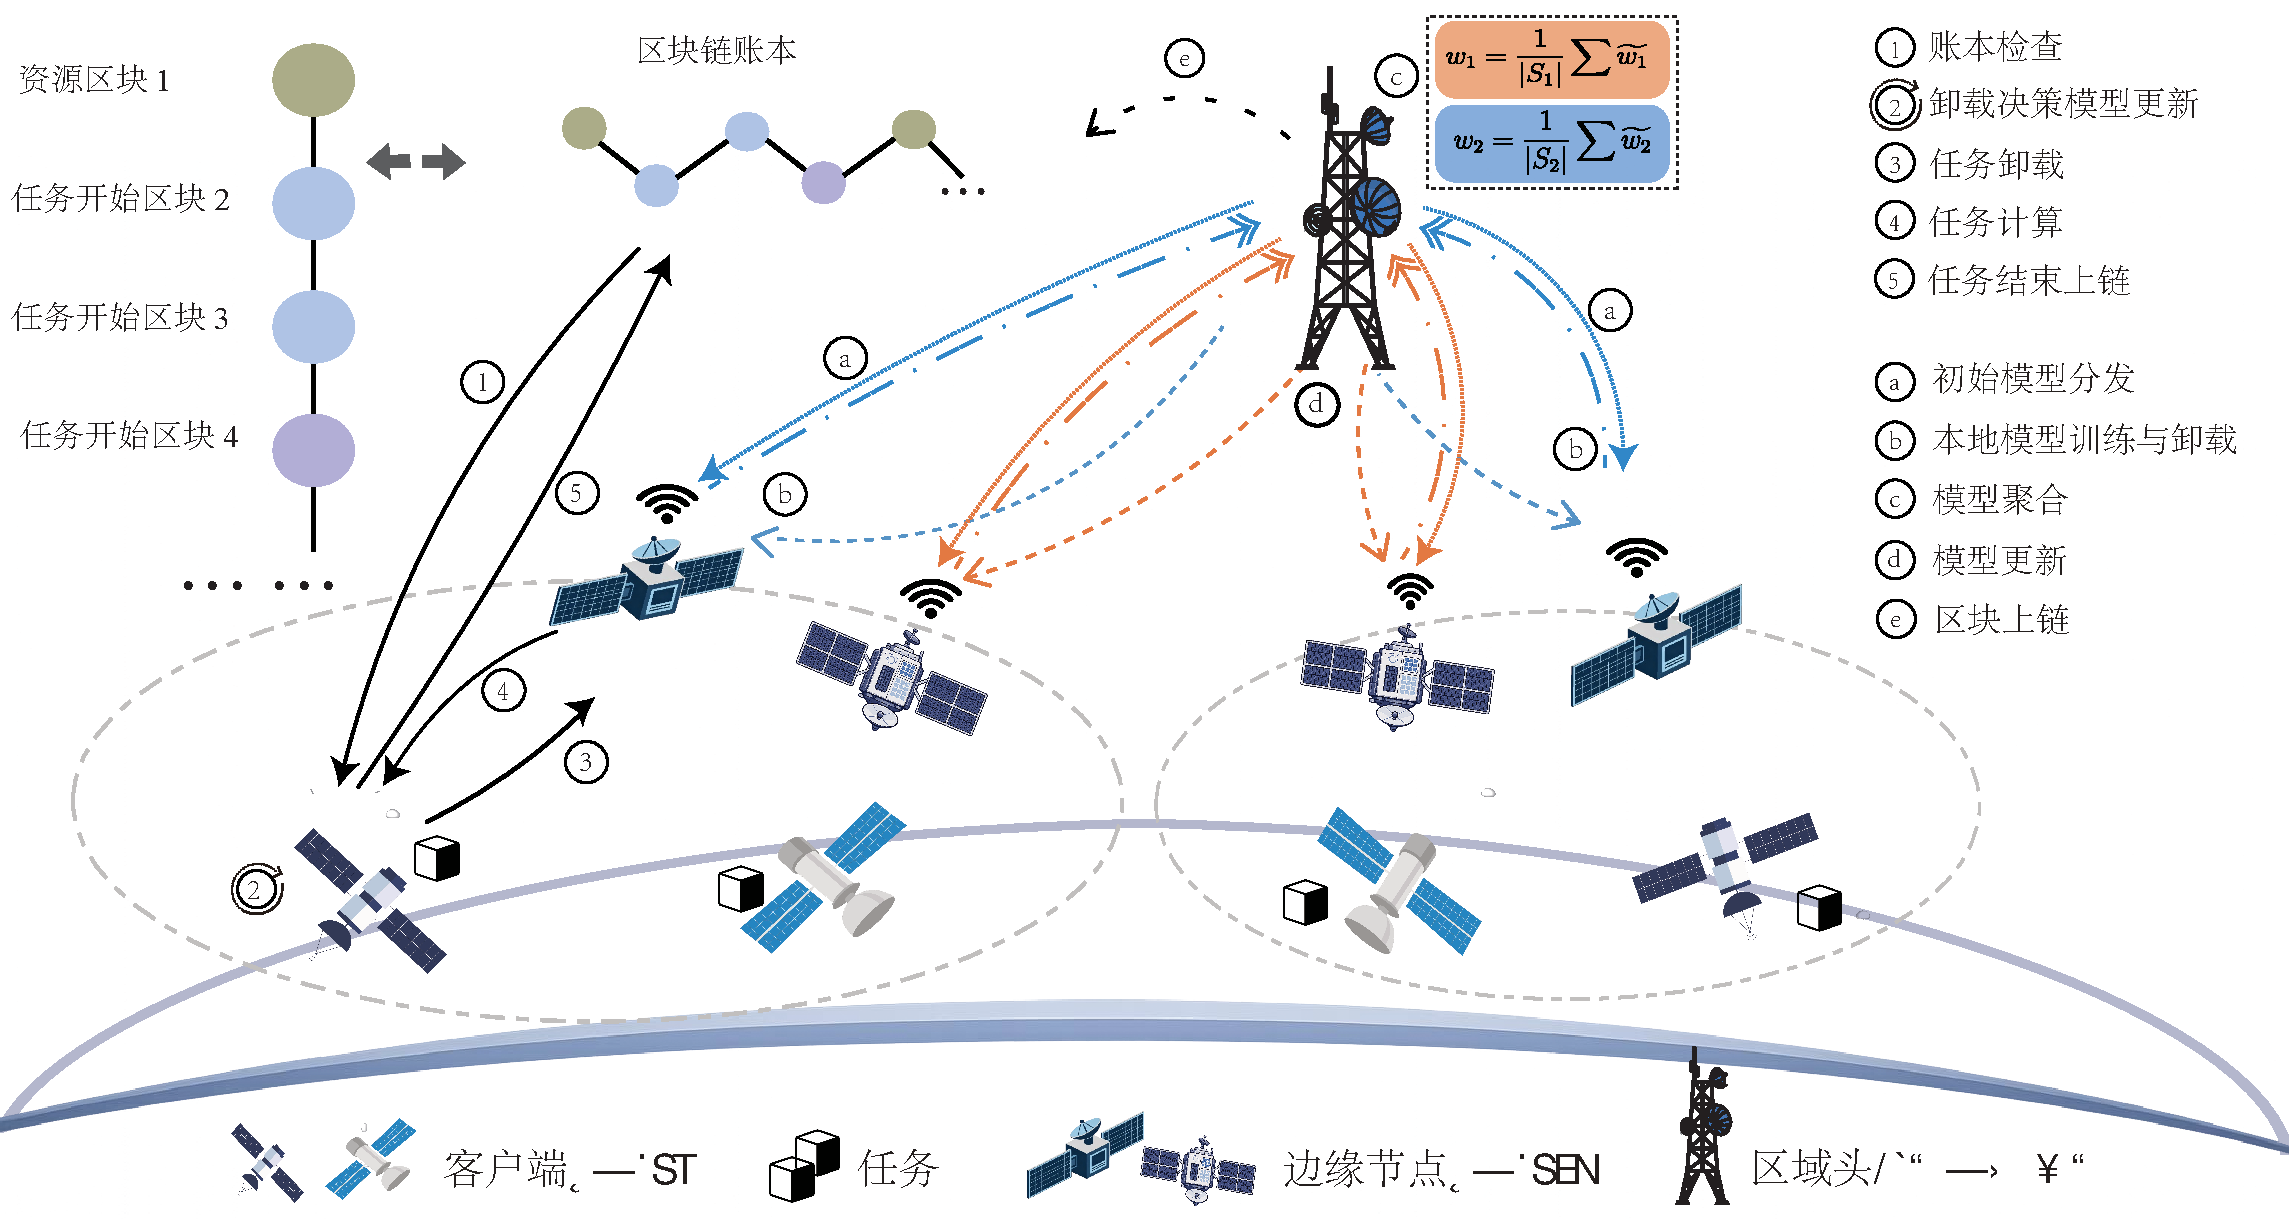
\includegraphics[width=0.95\textwidth]{figures/4-2.pdf}
    \caption{任务级卸载的系统级双闭环架构与信息交互流程}
    \label{fig:system_framework}
\end{figure}

在该系统级架构中，联盟链并不直接替代终端执行实时卸载决策，而是提供可信但非实时的公共摘要和模型版本凭据；联邦协调单元也不直接接管任务执行，而是在后台完成预测模型的簇内聚合与可信下发。为了使系统角色更清晰，表~\ref{tab:role_division} 总结了任务级卸载框架中的主要参与者及其职责。

\begin{table}[H]
    \centering
    \caption{任务级卸载框架中的角色划分}
    \label{tab:role_division}
    \begin{tabular}{p{2.5cm}p{8.8cm}}
        \toprule
        角色         & 主要职责                                               \\
        \midrule
        卫星终端 ST    & 生成新任务、采集本地 CPU/队列/剩余能量状态、读取链上摘要、触发并发开销预测并执行本地/卸载动作 \\
        卫星边缘节点 SEN & 接收外部任务、维护执行队列、反馈任务完成状态、沉淀历史执行日志并参与联邦训练             \\
        联盟链控制平面    & 维护候选节点公共摘要、任务开始/结束事件、模型版本号与哈希摘要，提供异步非实时全局视图        \\
        联邦协调单元     & 根据负载模式进行簇划分、完成簇内聚合与异常更新筛除、下发最新预测模型                 \\
        DQN 决策代理   & 将任务特征、本地状态、链上摘要和预测先验映射为离散卸载动作，并通过经验回放持续优化策略        \\
        \bottomrule
    \end{tabular}
\end{table}

从任务生命周期看，节点侧卸载决策遵循如下闭环流程：1）新任务到达后，终端提取计算量、输入规模、截止期与优先级等属性；2）终端同步采样本地资源状态，并从联盟链读取候选节点的公共摘要；3）调用候选目标所属簇的联邦预测模型，对各候选动作对应的并发开销进行快速估计；4）将任务特征、本地观测、链上摘要和预测先验拼接为统一状态向量；5）由 DQN 输出本地执行或目标节点卸载动作；6）环境返回真实时延、能耗和任务完成结果，并反向写入经验回放池；7）任务开始/结束事件与模型版本摘要继续在链上更新，构成“决策—执行—反馈—再决策”的闭环。该流程与图~\ref{fig:system_framework} 中的系统级信息流保持一致，即先由可信共享与联邦维护提供背景支撑，再由节点侧完成面向单任务的实时决策。

对任意时刻到达终端的一个新任务，记其描述为
\begin{equation}
    T_i = \left(C_i,\, S_i,\, D_i,\, \tau_i,\, \zeta_i \right),
    \label{eq:task_tuple}
\end{equation}
其中，$C_i$ 表示任务计算量，$S_i$ 表示输入数据大小，$D_i$ 为最大可接受完成时延或截止期，$\tau_i$ 为任务类型编码，$\zeta_i$ 为任务优先级。这里使用 $D_i$ 表示时延约束，是为了避免与任务符号 $T_i$ 发生混淆。

与第三章的系统层全局建模不同，本章关注的是{单任务在到达瞬间面临的局部动作选择}。设候选动作集合为
\begin{equation}
    \mathcal{A} = \left\{0,1,2,\ldots,N_c\right\},
    \label{eq:action_set}
\end{equation}
其中，动作 $0$ 表示本地执行，动作 $n \in \{1,\ldots,N_c\}$ 表示卸载至第 $n$ 个可达候选边缘节点。节点侧决策需要在一个极短时间窗口内完成，因此策略不仅要追求高质量，还要具备较低的在线推理开销。

为支撑后续奖励函数和评价指标设计，本节先给出单任务在本地执行和边缘卸载两种情形下的时延、能耗模型。

若任务在本地执行，则其完成时延由本地等待时延和本地计算时延共同构成：
\begin{equation}
    L_i^{\mathrm{loc}}(t) = W_i^{\mathrm{loc}}(t) + \frac{C_i}{f_i^{\mathrm{loc}}(t)},
    \label{eq:local_delay}
\end{equation}
其中，$W_i^{\mathrm{loc}}(t)$ 表示任务进入本地队列后的等待时间，$f_i^{\mathrm{loc}}(t)$ 为终端在当前时刻可分配给该任务的有效计算频率。相应地，本地执行能耗可写为
\begin{equation}
    E_i^{\mathrm{loc}}(t) = \kappa_i C_i \left( f_i^{\mathrm{loc}}(t) \right)^2
    + P_i^{\mathrm{idle}} W_i^{\mathrm{loc}}(t),
    \label{eq:local_energy}
\end{equation}
其中，$\kappa_i$ 为设备有效电容系数，$P_i^{\mathrm{idle}}$ 用于近似本地等待期间的空闲维持功耗。若不考虑本地排队或等待能耗，上式可退化为常见的动态功耗模型。

若任务卸载到候选边缘节点 $n$，则其端到端完成时延可分解为上行传输时延、传播时延、边缘基础排队时延、边缘计算时延和并发扰动时延五部分，即
\begin{equation}
    L_i^{\mathrm{off}}(n,t) = \frac{S_i}{R_{i,n}^{\mathrm{up}}(t)} + d_{i,n}^{\mathrm{prop}}(t)
    + W_{n}^{\mathrm{edge}}(t) + \frac{C_i}{F_n(t)} + \Delta_i(n,t),
    \label{eq:offload_delay}
\end{equation}
其中，$R_{i,n}^{\mathrm{up}}(t)$ 为上行传输速率，$d_{i,n}^{\mathrm{prop}}(t)$ 为传播时延，$W_{n}^{\mathrm{edge}}(t)$ 为不考虑新任务扰动时目标节点已有队列造成的基础等待时间，$F_n(t)$ 为目标节点当前可用计算能力，$\Delta_i(n,t)$ 为将新任务放置到节点 $n$ 后额外产生的并发开销。该写法将“已有队列导致的常规等待”和“新任务加入后造成的资源竞争扰动”分开，有助于后续突出并发开销预测模块的作用。

相应地，卸载能耗可写为
\begin{equation}
    E_i^{\mathrm{off}}(n,t) = P_i^{\mathrm{tx}}\frac{S_i}{R_{i,n}^{\mathrm{up}}(t)}
    + P_i^{\mathrm{idle}}\left(d_{i,n}^{\mathrm{prop}}(t)+W_{n}^{\mathrm{edge}}(t)\right)
    + \eta_n \frac{C_i}{F_n(t)},
    \label{eq:offload_energy}
\end{equation}
其中，$P_i^{\mathrm{tx}}$ 为终端发射功率，$\eta_n$ 为将目标节点执行能耗折算回任务代价的系数。式~(\ref{eq:offload_energy}) 不仅刻画了传输能耗，也保留了等待和边缘侧执行的代价信息，从而避免策略一味追求低时延卸载而忽略系统整体能源消耗。

在进一步建模之前，有必要说明本章变量的来源与适用边界。任务计算量、输入数据规模、截止期和优先级来自业务层任务描述；本地 CPU 占用、队列长度、剩余能量和可用频率由终端实时采样获得；候选节点平均负载、负载方差、信誉评分和模型版本号等信息来自联盟链维护的公共摘要；执行中任务剩余工作量、上下文切换强度和资源争用统计由边缘节点日志离线统计获得，并在联邦训练阶段转化为监督样本。与此同时，式~(\ref{eq:offload_delay}) 与式~(\ref{eq:offload_energy}) 建立在几个工程假设之上：其一，任务到达可用泊松流或离散事件过程近似；其二，边缘节点在短时间窗内的标称算力变化相对平缓；其三，链上摘要虽然可能存在陈旧性，但版本顺序和摘要内容是可信的。后续实验中的链上滞后敏感性分析，正是对上述假设边界进行专门验证。

\subsection{并发开销建模}

并发开销是本章区别于传统卸载模型的关键变量。设在时刻 $t$，目标节点 $n$ 上已有执行中任务集合 $\mathcal{T}_{n}^{\mathrm{exec}}(t)$，新任务 $T_i$ 被放置到该节点后，系统会因 CPU 时间片争用、缓存冲突、内存带宽竞争和 I/O 排队而出现额外时延。为了同时刻画新任务自身被拖慢和存量任务被扰动两类影响，将任务 $T_i$ 产生的并发开销定义为
\begin{equation}
    CO_i(n,t) =
    \left[L_i^{\mathrm{conc}}(n,t)-L_i^{\mathrm{base}}(n,t)\right]
    + \sum_{e \in \mathcal{T}_{n}^{\mathrm{exec}}(t)}
    \left[\widetilde{L}_{e}^{\mathrm{conc}}(n,t)-\widetilde{L}_{e}^{\mathrm{base}}(n,t)\right],
    \label{eq:co_formal}
\end{equation}
其中，$L_i^{\mathrm{base}}(n,t)$ 表示新任务在目标节点不受额外并发扰动时的基准完成时延，$L_i^{\mathrm{conc}}(n,t)$ 表示新任务加入真实并发环境后的完成时延；$\widetilde{L}_{e}^{\mathrm{base}}(n,t)$ 表示存量任务 $e$ 在没有新任务 $T_i$ 加入时的预计剩余完成时延，$\widetilde{L}_{e}^{\mathrm{conc}}(n,t)$ 表示新任务加入后该存量任务的剩余完成时延。与只关注新任务自身时延的定义相比，式~(\ref{eq:co_formal}) 同时计入了新任务进入成本与存量任务受扰成本，因此更符合节点侧真实的资源竞争机制。

图~\ref{fig:co_illustration} 展示了并发开销的形成机理。该图应与式~(\ref{eq:co_formal}) 对应理解：左侧表示无新任务加入时存量任务按相对稳定的资源份额推进；右侧表示新任务进入后，CPU、Cache、Memory 和 I/O 等共享资源被重新分配，存量任务出现受扰延迟，新任务也因竞争产生额外等待。因而，并发开销不是单个任务的固定附加项，而是由任务组合、资源瓶颈和执行上下文共同决定的耦合代价。

\begin{figure}[H]
    \centering
    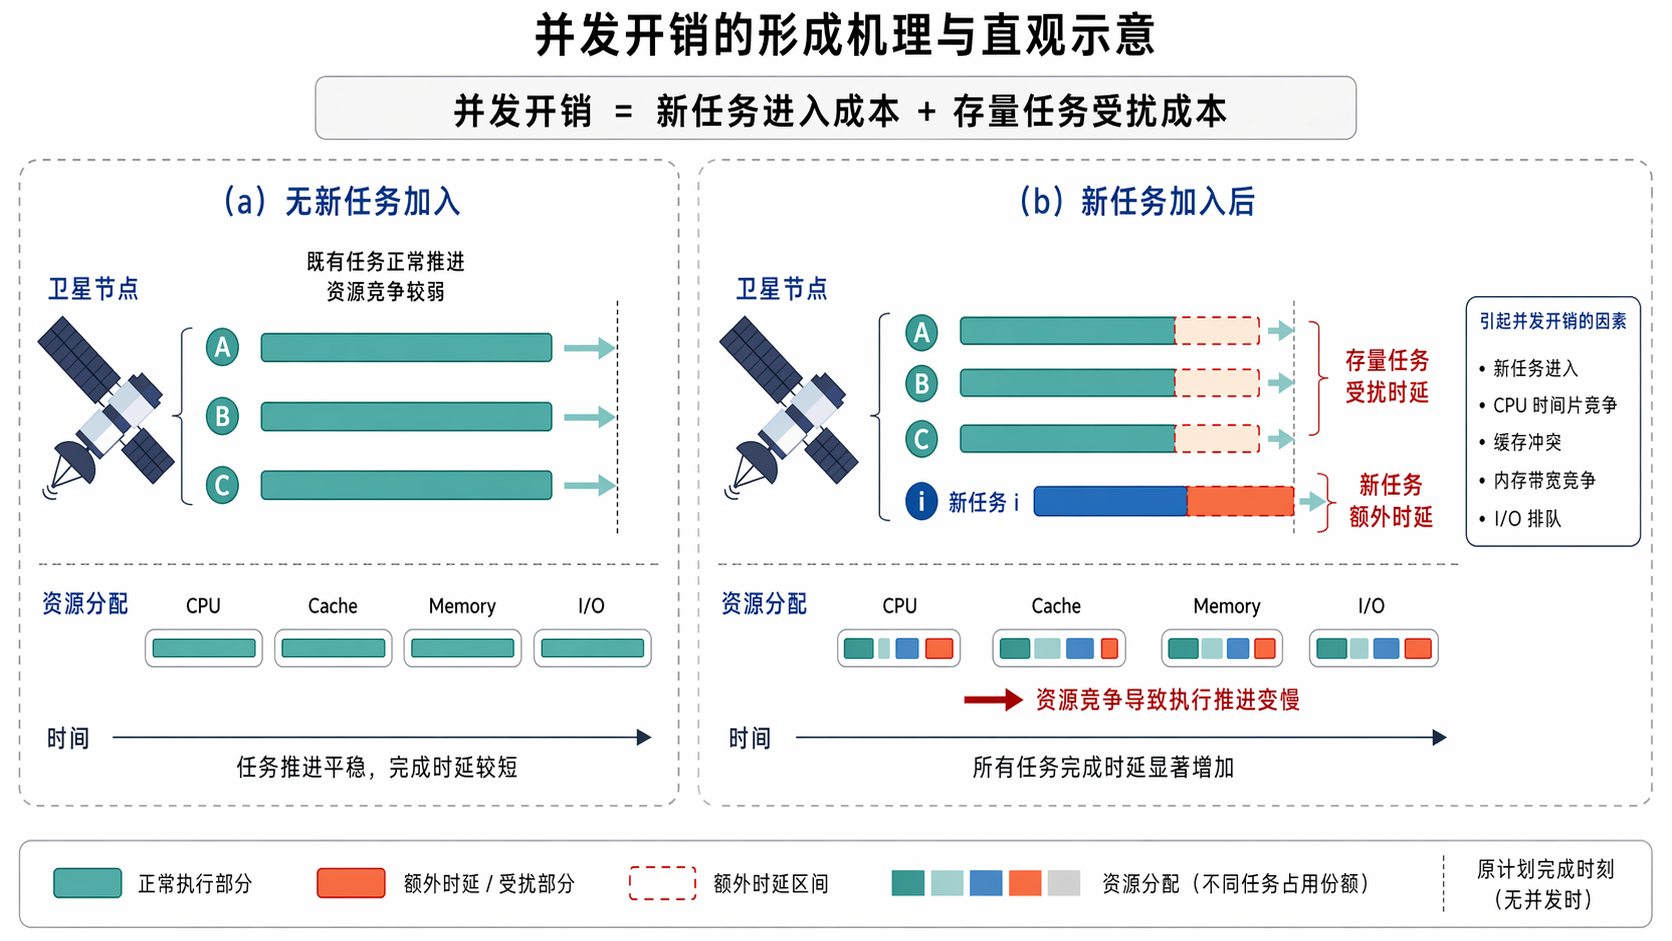
\includegraphics[width=0.92\textwidth]{figures/4-3.png}
    \caption{并发开销的形成机理与资源争用示意}
    \label{fig:co_illustration}
\end{figure}

在工程实现中，式~(\ref{eq:co_formal}) 所涉及的未来并发时延难以在决策瞬间直接获得，因此还需构造一个可学习、可预测的近似表达。记目标节点当前并发任务数为 $k_n(t)$，节点当前可用计算能力为 $F_n(t)$，执行中任务 $e$ 的剩余计算量为 $C_e^{\mathrm{rem}}(t)$，并用 $\chi_{i,e}\in[0,1]$ 表示新任务与存量任务在资源需求类型上的竞争强度，则并发扰动可近似写为
\begin{equation}
    \Delta_i(n,t) \approx \frac{\left(k_n(t)-1\right)C_i}{F_n(t)}
    + \sum_{e \in \mathcal{T}_{n}^{\mathrm{exec}}(t)}
    \frac{\chi_{i,e} C_e^{\mathrm{rem}}(t)}{F_n(t)},
    \label{eq:co_approx}
\end{equation}
该表达式揭示了并发开销与新任务计算量、当前并发任务数、存量任务剩余工作量以及任务间资源竞争强度之间的正相关关系，便于在后续样本标注、特征选择和模型解释中使用。当缺少细粒度资源画像时，可令 $\chi_{i,e}=1$ 得到保守估计。

进一步地，从统计学习角度可以将并发开销写为
\begin{equation}
    CO_i(n,t) \approx F_{\mathrm{new}}(T_i,n,\mathrm{obs})
    + G_{\mathrm{exec}}(\mathcal{T}_{n}^{\mathrm{exec}}(t),n,\mathrm{obs})
    + R_i(n,t),
    \label{eq:co_decomp}
\end{equation}
其中，$F_{\mathrm{new}}(\cdot)$ 捕获新任务加入带来的瞬时冲击，$G_{\mathrm{exec}}(\cdot)$ 刻画已执行任务间的持续资源竞争，$R_i(n,t)$ 表示未建模的高阶耦合残差。该可分解表达虽不直接用于在线推理，却有助于解释为何联邦模型在轻负载和重负载场景下会表现出不同的误差模式：前者更依赖新任务特征，后者更依赖存量任务组合和运行背景。

考虑时延、能耗和并发扰动三类代价，本章将动作 $a_t$ 对应的单任务总代价定义为
\begin{equation}
    J_i(a_t) = \omega_L L_i(a_t) + \omega_E E_i(a_t) + \omega_C \Delta_i(a_t),
    \qquad
    \omega_L+\omega_E+\omega_C=1,
    \label{eq:total_cost}
\end{equation}
其中，$L_i(a_t)$ 为动作执行后的端到端完成时延，$E_i(a_t)$ 为对应能耗，$\Delta_i(a_t)$ 表示动作引起的并发扰动；对于本地执行动作，可令 $\Delta_i(a_t)$ 表示本地队列中存量任务受到的额外扰动，也可在只关注边缘并发时取零。三个权重参数可根据业务偏好灵活调整：对实时业务可提高 $\omega_L$，对能源敏感任务可提高 $\omega_E$，对高拥塞控制场景则可适当增加 $\omega_C$。采用 $\omega$ 作为代价权重，是为了避免与后续 DQN 中的折扣因子符号混用。

值得指出的是，式~(\ref{eq:total_cost}) 的意义并不仅在于给出加权求和目标，更重要的是为后续 DQN 奖励函数设计提供统一的任务层优化视角。第三章关注的是系统层的全局资源配置，本章则将优化边界收缩到{节点侧单任务决策}，从而在保持整体方法链连贯性的同时，避免重复求解上一章已经讨论过的系统层全局资源调度问题。

\subsection{状态表征构造}

为了使并发开销能够被机器学习模型预测，并使 DQN 能够进行可执行的在线决策，需要构造一个统一的复合状态表征。设可观测特征向量为
\begin{equation}
    \bm{x} = \left[ \bm{x}^{\mathrm{task}},\,
        \bm{x}^{\mathrm{local}},\,
        \bm{x}^{\mathrm{chain}},\,
        \bm{x}^{\mathrm{conc}}
        \right],
    \label{eq:feature_vector}
\end{equation}
其中：
\begin{itemize}[leftmargin=2.5em]
    \item $\bm{x}^{\mathrm{task}}$：新任务特征，包括计算量、输入大小、时延阈值、任务类型编码、优先级等；
    \item $\bm{x}^{\mathrm{local}}$：本地状态，包括本地 CPU 占用、队列长度、剩余能量、可用频率和链路质量估计等；
    \item $\bm{x}^{\mathrm{chain}}$：链上公共摘要，包括候选节点平均负载、负载方差、信誉评分、账本确认延迟估计等；
    \item $\bm{x}^{\mathrm{conc}}$：并发环境统计，包括目标节点当前并发任务数、执行中任务总剩余工作量、平均内存占用和上下文切换强度等。
\end{itemize}

所有连续特征在进入模型前都进行标准化处理，即
\begin{equation}
    \tilde{x}_j = \frac{x_j - \mu_j}{\sigma_j + \varepsilon},
    \label{eq:normalize}
\end{equation}
其中，$\mu_j$ 和 $\sigma_j$ 分别为训练集统计均值和标准差，$\varepsilon$ 为数值稳定常数。

需要强调的是，节点侧状态天然是不完全的：一方面，本地节点只能直接观测自身状态，无法获取其他候选节点的细粒度实时运行轨迹；另一方面，链上摘要虽然提供了全网一致视图，但其时间戳可能早于当前决策时刻。因此，本章所研究的卸载问题本质上是在{部分可观测、带滞后信息的动态环境}下进行的序贯决策问题。引入 FL 预测模块的意义，正是在不可能获得完整实时信息的前提下，用历史数据学习出的风险先验来弥补观测缺口。

\subsection{任务层卸载问题的马尔可夫决策过程建模}

在上述基础上，节点侧任务卸载被建模为马尔可夫决策过程
\begin{equation}
    \mathcal{M} = \langle \mathcal{S}, \mathcal{A}, \mathcal{P}, \mathcal{R} \rangle.
\end{equation}
其中：
\begin{itemize}[leftmargin=2.5em]
    \item 状态空间 $\mathcal{S}$ 由任务特征、本地资源状态、链上公共摘要和 FL 预测值共同组成；
    \item 动作空间 $\mathcal{A}$ 为“本地执行 + 若干候选 SEN”构成的离散集合；
    \item 状态转移概率 $\mathcal{P}$ 由任务到达、链路变化、资源占用演化和预测结果更新共同决定；
    \item 奖励函数 $\mathcal{R}$ 采用总代价负值并叠加轻量奖惩项。
\end{itemize}

为了便于工程部署，本章选择基于离散动作值函数的 DQN，而没有采用连续动作策略梯度类方法，主要原因有二：其一，本场景的动作集合有限，DQN 推理效率高、实现成本低；其二，本章更希望把模型复杂度预算留给“并发开销预测”这一难点环节，而非在在线阶段引入过于复杂的连续动作网络。

\section{基于联邦学习的并发开销预测方法}
\label{sec:fl_prediction}
在上一节完成任务层代价建模之后，本节进一步回答“并发开销如何在隐私受限和样本异构条件下被有效学习”这一问题。按照“预测目标—模型结构—联邦训练—可信维护”的链式逻辑，本节首先说明监督样本如何从执行日志中构造，其次给出预测器为什么采用轻量 MLP/1D-CNN 结构，再介绍聚类式联邦训练为何优于统一 FedAvg，最后讨论模型版本如何借助联盟链进行可信维护与在线调用。这样的组织方式与参考章节中“框架概述之后再逐层展开算法设计”的写法保持一致，便于读者把每个模块放回整体系统闭环中理解。

\subsection{预测目标与样本构造}

并发开销预测本质上是一个监督回归问题。其输入为式~(\ref{eq:feature_vector}) 定义的多维特征，输出为目标节点在接受新任务后的并发开销估计值 $\widehat{\Delta}$ 及其置信信息。设节点本地构造的监督样本为
\begin{equation}
    \mathcal{D}_k = \left\{ \left(\bm{x}^{(m)}, y^{(m)} \right) \right\}_{m=1}^{N_k},
\end{equation}
其中，$y^{(m)}$ 为根据运行日志标注得到的真实并发开销。对于每个样本，需要记录任务到达前后的队列长度、CPU 频率、内存占用、任务开始时间、完成时间、输入大小、计算量等信息，再依照式~(\ref{eq:co_formal}) 或式~(\ref{eq:co_approx}) 计算标签。

为了使预测模型尽可能覆盖多样化的竞争形态，本章沿用原稿中的“双代理负载”的思路：一类是图像处理任务，用于模拟视觉感知类边缘业务；另一类是数值计算任务，用于模拟计算密集但数据规模较小的负载。这种设计的好处在于，既能让模型观察到数据搬移开销与计算开销同时占优的混合场景，又能避免训练集完全偏向单一类型任务而失去泛化性。

\subsection{预测模型结构设计}

考虑到输入特征既包含结构化统计量，也可能包含短时间窗内的序列信息，本章在模型结构上兼容两类实现：

\begin{enumerate}[label=\arabic*)]
    \item {MLP 结构}：适用于结构化向量输入。模型通常由 3--5 个全连接隐藏层构成，每层采用 ReLU 激活并可结合 Dropout 抑制过拟合；
    \item {1D-CNN 结构}：当输入拼接了过去若干时间步的 CPU 利用率、队列长度或链路质量序列时，1D-CNN 可以提取时序局部模式，再通过全连接层输出最终预测值。
\end{enumerate}

为了使预测结果能够在决策阶段发挥更稳健的作用，本章进一步采用{均值 + 方差双输出}的设计，即网络输出
\begin{equation}
    f_{\theta}(\bm{x}) = \left(\widehat{\Delta},\, \widehat{\sigma}^2 \right),
\end{equation}
其中，$\widehat{\Delta}$ 为并发开销点估计，$\widehat{\sigma}^2$ 为预测方差估计。与只输出单一标量相比，增加不确定性分支具有两方面价值：一是便于在 DQN 状态中引入“模型对该预测是否有把握”的额外信息；二是在高异构、弱覆盖样本区间内，不确定性可以提醒策略避免过度依赖单一预测值。

从实现角度看，预测器本身不追求过深或过重的网络结构，而强调对结构化特征、短时间窗统计序列以及不确定性信息的统一表达。也正因为本章的重点在于“并发风险感知如何服务任务级决策”，所以模型结构仅保留轻量、可部署和可解释的设计原则，而不将网络复杂度本身作为主要创新点。

在损失函数设计上，若仅关注点估计，可使用均方误差
\begin{equation}
    \mathcal{L}_{\mathrm{MSE}} = \frac{1}{N}\sum_{m=1}^{N}
    \left( \widehat{\Delta}^{(m)} - \Delta^{(m)} \right)^2.
    \label{eq:mse_loss}
\end{equation}
若同时训练不确定性分支，则可以采用异方差高斯负对数似然形式
\begin{equation}
    \mathcal{L}_{\mathrm{pred}}
    =
    \frac{1}{N}
    \sum_{m=1}^{N}
    \left[
        \frac{\left(\widehat{\Delta}^{(m)}-\Delta^{(m)}\right)^2}{2\widehat{\sigma}^{2(m)}}
        +
        \frac{1}{2}\log \widehat{\sigma}^{2(m)}
        \right].
    \label{eq:hetero_loss}
\end{equation}
该损失函数允许模型在噪声较大的区域给出更高的不确定性估计，从而避免对本就难以准确预测的样本过度拟合。

\subsection{分层聚类联邦架构与训练流程}

由于不同边缘卫星节点的本地样本分布具有显著 Non-IID 特征，直接使用统一的 FedAvg 训练单一全局模型往往难以兼顾不同簇之间的局部负载模式。基于此，本文采用聚类式联邦学习（clustered FL）对预测模型进行训练。其核心思路是：不再假设全网节点共享同一个最优模型，而是先根据节点负载模式、硬件能力或更新方向将其划分为多个簇，再在簇内执行模型聚合。

面向天基网络的层次化结构，本章将联邦预测框架设计为“全局协调层—区域聚合层—本地训练层”三层架构。与参考章节中“系统组成—工作流程—算法设计”的写法一致，这里先说明各层角色，再给出训练流程与簇内聚合规则。

三层架构的职责分工如表~\ref{tab:fl_roles} 所示。

\begin{table}[H]
    \centering
    \caption{分层聚类联邦学习架构中的角色划分}
    \label{tab:fl_roles}
    \begin{tabular}{p{2.7cm}p{3.0cm}p{6.0cm}}
        \toprule
        层级    & 典型实体           & 主要职责                           \\
        \midrule
        全局协调层 & 地面控制中心 / 星座控制器 & 模型版本管理、训练轮次调度、簇级模型下发、链上摘要维护    \\
        区域聚合层 & 核心边缘卫星节点       & 区域内节点分组、异常更新检测、簇内参数加权聚合        \\
        本地训练层 & 参与训练的 SEN 集合   & 基于本地执行日志训练预测模型，不上传原始样本，仅上传模型更新 \\
        \bottomrule
    \end{tabular}
\end{table}

在一次完整的联邦训练周期内，预测模型的工作流程可以概括为：1）全局协调层根据节点历史负载模式完成簇划分并下发初始化模型；2）本地训练层在各自执行日志上完成若干轮本地更新；3）区域聚合层对上传参数执行一致性检查、异常更新筛除与簇内加权聚合；4）聚合后的模型版本号和参数哈希写入联盟链，供后续在线推理时进行版本校验与追溯；5）最新簇模型再次下发至簇内节点，进入下一轮训练。上述流程使预测模型的训练、维护和可信存证形成统一闭环。

设第 $c$ 个簇内包含若干节点集合 $C_c$，第 $t$ 轮通信后簇模型参数更新为
\begin{equation}
    \theta_c^{(t+1)} =
    \sum_{k \in C_c}
    \frac{n_k}{\sum_{j \in C_c}n_j}
    \theta_k^{(t+1)},
    \label{eq:cluster_fedavg}
\end{equation}
其中，$n_k$ 为节点 $k$ 的本地样本量，$\theta_k^{(t+1)}$ 为节点本地更新后的参数。与传统 FedAvg 相比，式~(\ref{eq:cluster_fedavg}) 的改进并不体现在加权形式本身，而在于聚合只在“样本分布相近的节点簇内”进行，因此更容易捕捉局部任务模式。

在实现层面，聚类式联邦训练不只是“把 FedAvg 换成簇内 FedAvg”，还需要把训练过程与区块链提供的可信机制结合起来。具体而言，区域聚合层在每轮簇内聚合后，可将模型版本号、参数哈希和训练轮次摘要写入联盟链，用于完成模型溯源、版本一致性校验与异常更新留痕；终端节点在调用预测器时只需读取候选节点当前所属簇的最新可用模型版本，从而避免在在线阶段访问原始训练日志。这样的设计使“数据不出域”和“模型可追溯”同时成立，也使预测模块更容易并入第三章已经建立的可信协同框架中。

聚类式联邦学习的一个完整训练轮次可由算法~\ref{alg:clusterfedavg} 概括。相较原始 FedAvg，该流程新增了簇内聚合、异常更新筛查与链上存证三个关键步骤，因此更适合 Non-IID 且可信要求较高的天基边缘场景。

\begin{algorithm}[H]
    \caption{聚类式联邦学习（Clustered FedAvg）训练流程}
    \label{alg:clusterfedavg}
    \small
    \begin{algorithmic}[1]
        \Statex {输入：}簇划分集合 $\{C_1,\ldots,C_K\}$，本地数据集 $\mathcal{D}_k$，本地训练轮数 $E$，通信轮数 $T$。
        \Statex {输出：}各簇最终预测模型参数 $\theta_c^{(T)}$。
        \For{每个簇 $C_c$}
        \State 初始化簇模型参数 $\theta_c^{(0)}$ 并下发至簇内节点
        \EndFor
        \For{$t=0,1,\ldots,T-1$}
        \For{每个簇 $C_c$ 并行执行}
        \For{每个参与节点 $k\in C_c$}
        \State 以 $\theta_c^{(t)}$ 为初值，在 $\mathcal{D}_k$ 上执行 $E$ 个 epoch 本地更新
        \State 得到本地参数 $\theta_k^{(t+1)}$ 及样本量 $n_k$
        \EndFor
        \State 区域聚合层对上传更新做一致性检查与异常筛除
        \State 按式~(\ref{eq:cluster_fedavg}) 聚合得到新的簇模型 $\theta_c^{(t+1)}$
        \State 将模型版本号、参数哈希及训练轮次摘要写入联盟链
        \EndFor
        \EndFor
    \end{algorithmic}
\end{algorithm}

在线推理阶段，终端节点并不直接参与联邦训练，而是在需要决策时调用候选边缘节点所属簇的最新预测模型，对每个候选动作的并发开销进行快速估计。这一点十分重要：联邦学习的高开销发生在离线训练或后台异步更新阶段，而在线阶段保留下来的只是一个轻量前向推理过程，因此不会破坏节点侧决策的实时性要求。

\subsection{可信维护与复杂度分析}

从时间复杂度看，若单个本地预测模型包含 $P_f$ 个参数，本地每轮训练使用 $B_f$ 个 mini-batch，则节点单轮本地训练复杂度约为 $\mathcal{O}(B_f P_f)$；簇内聚合本质是参数加权求和，复杂度为 $\mathcal{O}(|C_c|P_f)$。由于聚类式 FL 把全局聚合分解为多个簇内聚合过程，单轮同步对全网连通性的要求低于统一 FedAvg。相比之下，在线阶段仅保留一次前向推理，因此预测模块在部署时的主要成本不是计算本身，而是模型版本刷新与链上摘要读取的调度机制。

从通信复杂度看，联邦学习阶段每轮只需要在节点与聚合层之间传递参数摘要，而无需传递原始日志数据。在天基网络这类带宽和链路可用性受限的环境中，这种“模型移动而非数据移动”的设计具有明显优势。与此同时，聚类式 FL 还可以借助区域聚合层把大规模全局同步拆解成多个较小的局部同步过程，降低单轮训练对网络连通性的苛刻要求。

进一步地，若把模型可信维护纳入考虑，则每轮额外链上开销主要来自模型哈希写入和版本确认，这部分复杂度与模型参数规模无关，而与摘要长度和交易确认时延有关。因此，区块链并不会显著增加预测器训练的算力负担，但会通过信息年龄影响在线可用模型版本的新鲜度。后续实验中的“链上确认延迟敏感性”正是对这一现实部署约束的量化验证。

\section{FL-DQN 卸载决策算法设计}
\label{sec:dqn_policy}
如果说上一节解决的是“如何看见未来并发风险”，那么本节解决的便是“如何把这种风险感知转化为实时动作”。因此，本节不再重复描述预测模型本身，而是聚焦于节点侧决策代理如何读取预测先验、如何构造奖励约束、如何在在线阶段完成闭环交互，以及为什么该算法在工程上可实现。整体上，本节按照“状态—奖励—训练—在线执行—复杂度”的顺序展开，使算法描述与章节主线保持一致。

\subsection{状态、动作与奖励函数设计}

在获得并发开销预测能力后，节点侧仍需进一步解决“面对新任务应当本地执行还是卸载到哪个候选节点”的决策问题。本文将单个 ST 的卸载过程建模为 MDP，其状态向量定义为
\begin{equation}
    s_t =
    \left[
        s_t^{\mathrm{task}},\,
        s_t^{\mathrm{local}},\,
        s_t^{\mathrm{chain}},\,
        s_t^{\mathrm{FL}}
        \right],
    \label{eq:dqn_state}
\end{equation}
其中，$s_t^{\mathrm{task}}$ 包含任务计算量、数据规模、截止期、任务类型编码与优先级；$s_t^{\mathrm{local}}$ 包含本地 CPU 占用、队列长度、剩余能量与链路质量估计；$s_t^{\mathrm{chain}}$ 来自联盟链上的候选节点公共摘要；$s_t^{\mathrm{FL}}$ 则由并发开销预测模型给出，包括各候选动作的 $\widehat{\Delta}_i(n,t)$ 及其不确定性 $\widehat{\sigma}_i^2(n,t)$。

表~\ref{tab:state_space} 总结了复合状态空间的设计。

\begin{table}[H]
    \centering
    \caption{节点侧决策的复合状态空间设计}
    \label{tab:state_space}
    \begin{tabular}{p{3.1cm}p{5.8cm}p{3.0cm}}
        \toprule
        状态分量      & 主要内容                               & 作用            \\
        \midrule
        任务特征向量    & 任务计算量、输入数据大小、截止期、任务类型编码、优先级        & 刻画当前任务需求      \\
        本地资源与链路状态 & 本地 CPU 占用、队列长度、剩余能量、可用频率、链路时延与带宽估计 & 反映当前本地资源与通信条件 \\
        链上公共摘要    & 候选节点平均负载、负载方差、信誉评分、账本延迟估计          & 提供系统级非实时协同上下文 \\
        FL 预测先验   & 各候选动作的并发开销预测值与不确定性                 & 显式表征卸载后的额外风险  \\
        \bottomrule
    \end{tabular}
\end{table}

奖励函数在总代价负值的基础上引入轻量奖惩机制：
\begin{equation}
    r_t = -\left(
    \omega_L L_i^{\mathrm{obs}}
    + \omega_E E_i^{\mathrm{obs}}
    + \omega_C \Delta_i^{\mathrm{obs}}
    \right)
    - \lambda_b P_{\mathrm{imbalance}}
    - \lambda_u \overline{\sigma}_t
    + R_{\mathrm{succ}},
    \label{eq:reward}
\end{equation}
其中，$L_i^{\mathrm{obs}}$、$E_i^{\mathrm{obs}}$ 和 $\Delta_i^{\mathrm{obs}}$ 分别表示任务执行后观测到的真实时延、能耗和并发扰动；$P_{\mathrm{imbalance}}$ 表示负载不均衡惩罚项，用于抑制任务长期集中到少数高性能边缘节点；$\overline{\sigma}_t$ 表示当前被选动作或候选动作集合上的平均预测不确定性，用于避免策略在高不确定区域过度激进；$R_{\mathrm{succ}}$ 为任务在截止期内完成、满足优先级约束或成功避开高拥塞节点时给予的正向奖励。若真实并发扰动反馈具有延迟，训练时可先使用 $\widehat{\Delta}_i$ 作为即时奖励塑形项，并在任务完成后用 $\Delta_i^{\mathrm{obs}}$ 更新经验样本。这样既保留了预测先验对动作选择的前瞻作用，又避免把预测值误认为最终真实奖励。

从机制上看，FL 预测先验具有两重作用：其一，它作为扩展状态的一部分帮助智能体在动作选择前识别潜在拥塞；其二，它通过奖励塑形和不确定性惩罚影响训练过程，使策略在候选节点当前负载相近但未来并发风险不同的情况下更倾向于选择低风险动作。与此同时，$P_{\mathrm{imbalance}}$ 的引入使策略不再只追求单次动作收益，而是能够兼顾较长时间尺度上的节点利用均衡。

\subsection{Q 网络结构与训练策略}

由于动作空间是有限离散集合，本文采用 DQN 学习最优动作价值函数 $Q^*(s,a)$。令主网络参数为 $\theta_q$，目标网络参数为 $\theta_q^{-}$，DQN 的 Bellman 目标值写为
\begin{equation}
    y_t =
    r_t + \rho \max_{a'} Q(s_{t+1},a';\theta_q^-),
    \label{eq:bellman_target}
\end{equation}
损失函数为
\begin{equation}
    \mathcal{L}_{\mathrm{DQN}}(\theta_q) =
    \mathbb{E}_{(s_t,a_t,r_t,s_{t+1}) \sim \mathcal{B}}
    \left[
        \left(
        y_t - Q(s_t,a_t;\theta_q)
        \right)^2
        \right],
    \label{eq:dqn_loss}
\end{equation}
其中，$\mathcal{B}$ 为经验回放池，$\rho\in[0,1)$ 为折扣因子。这里将折扣因子记为 $\rho$，以避免与式~(\ref{eq:total_cost}) 中的代价权重混淆。

为提高训练稳定性，本章沿用标准 DQN 的三项关键机制：

\begin{enumerate}[label=\arabic*)]
    \item {经验回放}：将交互产生的样本打乱后重用，削弱序列相关性；
    \item {目标网络}：使用滞后更新的目标网络生成目标值，减少训练震荡；
    \item {$\varepsilon$-greedy 探索}：在探索与利用之间进行平衡，防止策略过早陷入局部最优。
\end{enumerate}

在网络结构上，考虑到状态维度相对有限且要求在线推理足够快，本文使用两层或三层全连接网络逼近 $Q(s,a;\theta)$，隐藏层采用 ReLU 激活。相比于更复杂的 dueling、double 或 attention 结构，这种配置在节点侧具有更低的实现门槛和推理开销，更符合“轻量快速决策”的系统定位。当然，在实验中我们仍保留增强型 DQN 变体作为对比基线，以检验“改进 DRL 结构”和“引入预测先验”两条路线的相对收益。

\subsection{在线决策流程与闭环机制}

本章的关键不在于单独提出一个联邦预测器，也不在于单独训练一个 DQN，而在于二者如何形成有效闭环。与图~\ref{fig:system_framework} 强调“系统级双闭环架构”不同，图~\ref{fig:closed_loop} 进一步收缩到单个任务到达后的节点侧在线决策过程：新任务到达后，节点先收集本地状态和链上摘要；随后调用候选节点对应簇的最新预测模型生成并发开销估计及其不确定性；这些预测结果与原始状态一起构成 DQN 的输入；DQN 输出动作后，环境返回真实时延、能耗和任务结果，再以奖励形式反哺后续策略更新。

\begin{figure}[H]
    \centering
    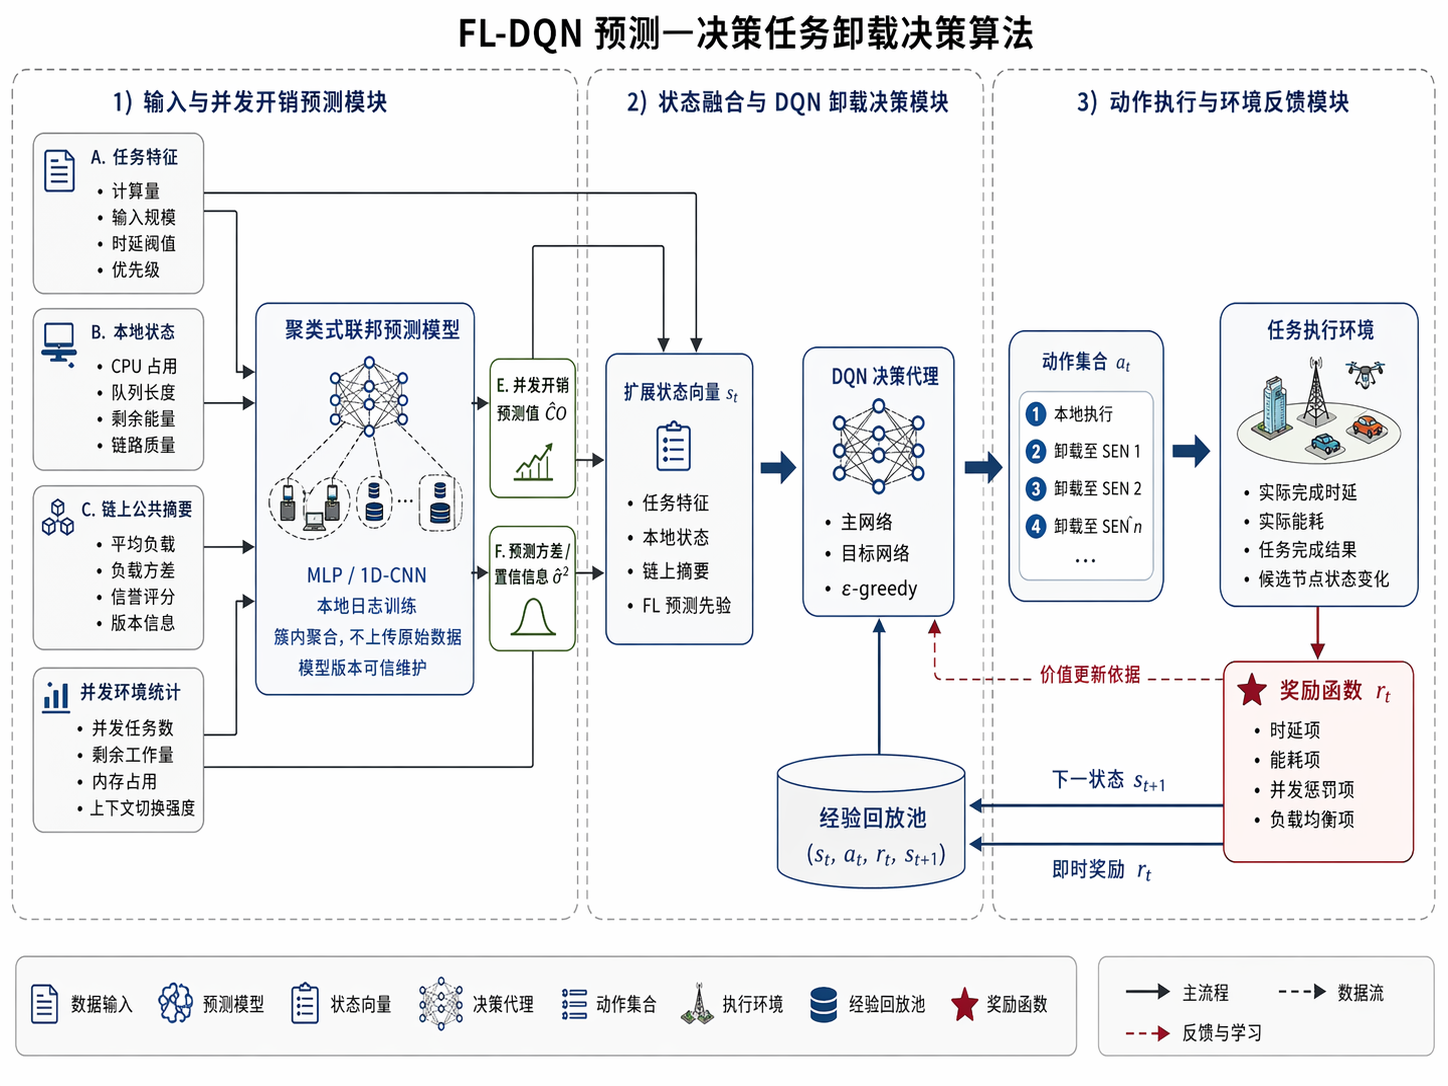
\includegraphics[width=0.96\textwidth]{figures/4-5.png}
    \caption{融合并发开销预测先验的 FL-DQN 在线卸载决策闭环}
    \label{fig:closed_loop}
\end{figure}

这种协同方式的优势在于，它把难以直接编码进解析策略的“未来并发风险”显式注入到了决策模块中。换言之，DQN 并不是在纯粹的即时观测之上做反应式决策，而是在带有预测先验的扩展状态上做前瞻式决策。特别是在高并发、链上状态滞后的场景中，这种差异通常会转化为更低的时延退化斜率和更好的系统鲁棒性。

综合上述设计，FL-DQN 在线卸载决策流程可概括为表~\ref{tab:online_policy} 所示的七个步骤。

\begin{table}[H]
    \centering
    \caption{FL-DQN 在线卸载决策流程}
    \label{tab:online_policy}
    \begin{tabular}{p{1.0cm}p{11.2cm}}
        \toprule
        步骤 & 流程描述                                                        \\
        \midrule
        1  & 终端节点接收新任务，提取计算量、数据大小、任务类型、优先级和截止期等特征。                       \\
        2  & 从本地环境读取 CPU、内存、队列长度、剩余能量与链路状态，并从联盟链获取候选边缘节点的公共摘要。           \\
        3  & 按候选目标节点所属簇调用联邦预测模型，对各候选动作的并发开销和预测不确定性进行快速推理。                \\
        4  & 将任务特征、本地资源状态、链上公共摘要和预测先验拼接为状态向量 $s_t$。                      \\
        5  & DQN 计算各动作的 $Q$ 值，并按 $\varepsilon$-greedy 规则选择本地执行或目标节点卸载动作。 \\
        6  & 环境返回任务完成时延、能耗、并发扰动和完成结果，据此计算奖励并写入经验回放池。                     \\
        7  & 主网络按 mini-batch 更新参数，目标网络按固定步长同步；策略持续与环境交互直至收敛。             \\
        \bottomrule
    \end{tabular}
\end{table}

为了更清楚地展示“预测先验如何进入在线动作选择”，算法~\ref{alg:fldqn_online} 对 FL-DQN 的节点侧执行流程给出伪代码描述。该伪代码与图~\ref{fig:closed_loop} 的区别在于：前者强调实现时的控制流，后者强调预测与决策之间的信息闭环。

\begin{algorithm}[H]
    \caption{FL-DQN 在线任务卸载决策流程}
    \label{alg:fldqn_online}
    \small
    \begin{algorithmic}[1]
        \Statex {输入：}最新可用联邦预测模型 $f_{\theta_f}$，DQN 主网络 $Q(\cdot;\theta_q)$，目标网络 $Q(\cdot;\theta_q^-)$，经验回放池 $\mathcal{B}$。
        \Statex {输出：}收敛后的节点侧卸载策略。
        \For{每个决策周期}
        \State 接收新任务并提取任务特征、本地资源状态与链上公共摘要
        \For{每个候选动作 $a\in\mathcal{A}$}
        \State 构造动作相关特征向量 $\bm{x}(s_t,a)$
        \State 调用 $f_{\theta_f}$ 得到并发开销预测值及不确定性 $\bigl(\widehat{\Delta}_i(s_t,a),\widehat{\sigma}_i^2(s_t,a)\bigr)$
        \EndFor
        \State 拼接得到扩展状态 $s_t$，按 $\varepsilon$-greedy 选择动作 $a_t$
        \State 执行动作并获得即时奖励 $r_t$ 与下一状态 $s_{t+1}$
        \State 将 $(s_t,a_t,r_t,s_{t+1})$ 写入经验回放池 $\mathcal{B}$
        \If{经验池样本数量足够}
        \State 从 $\mathcal{B}$ 随机采样 mini-batch，并按式~(\ref{eq:bellman_target}) 更新主网络
        \State 每隔固定步长同步目标网络参数 $\theta_q^- \leftarrow \theta_q$
        \EndIf
        \EndFor
    \end{algorithmic}
\end{algorithm}

\subsection{算法复杂度与可实现性分析}

对于单次在线决策，若候选边缘节点数量为 $N_c$，预测模型前向推理复杂度为 $\mathcal{O}(P_f)$，Q 网络前向推理复杂度为 $\mathcal{O}(P_q)$，则单次决策复杂度近似为
\begin{equation}
    \mathcal{O}\left(N_c P_f + P_q\right).
\end{equation}
由于 $N_c$ 通常远小于全网节点数，且 $P_f$ 和 $P_q$ 均来自轻量级 MLP/1D-CNN 结构，因此该复杂度满足节点侧实时部署需求。

若考虑训练阶段，则每次 DQN 参数更新需要对一个大小为 $B_q$ 的 mini-batch 执行前向与反向传播，复杂度约为 $\mathcal{O}(B_q P_q)$；经验回放池若容量为 $|\mathcal{B}|$，则其空间复杂度为 $\mathcal{O}(|\mathcal{B}|\,d_s)$，其中 $d_s$ 为状态维度。与引入预测先验所带来的性能收益相比，这部分额外存储开销是可控的。进一步地，预测模型本身可以异步更新，节点侧仅维护最近一次下发的模型副本，因此不会把联邦训练的成本直接叠加到每个在线动作上。

相比之下，若使用中心控制器收集全网细粒度状态再做统一决策，则不仅通信开销更高，而且难以满足天基网络中严格的时延约束。尤其是在链上状态存在确认延迟、候选节点可达性随轨道运动变化的条件下，把所有决策都放在中心完成会进一步放大信息年龄问题，而 FL-DQN 通过“链上摘要 + 本地观测 + 预测先验”的组合，能够在分布式条件下保留较高的动作质量。


\section{实验设计与结果分析}
\label{sec:experiments}

为系统验证所提 FL-DQN 任务卸载方法的有效性，本节按照“预测层验证—端到端性能验证—鲁棒性与可解释性分析—模块贡献分析”的逻辑展开实验。首先，通过并发开销预测精度、训练收敛过程、置信校准结果和异构环境下的预测误差，验证聚类式联邦学习能否为节点侧决策提供可靠的并发风险先验；其次，通过平均任务时延、系统吞吐量、SLA 完成率和 P99 尾时延等指标，分析预测先验是否能够有效转化为实际卸载收益；随后，从链上摘要陈旧性、动作选择偏好和效率--公平性折中三个角度进一步评估方法的鲁棒性与可解释性；最后，通过消融实验分析联邦预测模块、并发惩罚项、经验回放机制和奖励塑形项对整体性能的具体贡献。

需要说明的是，受限于真实在轨天基边缘计算环境难以直接部署和复现实验，本文实验部分采用模型驱动的离散事件仿真方式进行验证。仿真参数依据前文建立的任务层时延模型、能耗模型和并发开销模型设定，并结合图像处理类任务与数值计算类任务构造不同并发强度下的资源竞争场景。实验结果主要用于比较不同策略在相同约束条件下的相对性能差异，而不代表某一具体星载平台的绝对实测性能。

\subsection{实验场景、对比方法与评价指标}
\label{subsec:exp_setup}

实验场景模拟由若干卫星终端 ST、候选卫星边缘节点 SEN、联盟链控制平面和联邦协调单元共同组成的天基分布式计算系统。终端侧任务按照离散事件方式持续到达，每个任务包含计算量、输入数据大小、时延约束、任务类型和优先级等属性；候选边缘节点具有不同的计算能力、队列长度、背景负载和并发任务数；链上公共摘要以固定周期更新，用于提供候选节点的平均负载、负载方差、信誉评分和模型版本信息。为模拟天基网络中的状态滞后现象，实验进一步设置可控的链上摘要延时，并考察不同延时条件下各策略的性能变化。

并发开销预测数据由两类代理任务构造：一类为图像处理任务，用于模拟遥感预处理、轻量识别和视觉感知类边缘负载；另一类为数值计算任务，用于模拟输入规模较小但计算强度较高的计算密集型负载。每条样本记录任务类型、输入规模、估计计算量、节点 CPU 状态、并发任务数、执行中任务剩余工作量、上下文切换强度以及实际完成时延，并根据前文定义的并发开销表达式构造监督标签。这样既能够覆盖数据搬移和计算争用同时存在的混合场景，也能够避免训练样本过度偏向单一任务类型。

对比方法包括以下几类：{FL-DQN} 表示本文提出的完整方法；{DQN-only} 表示不引入联邦预测先验，仅依靠即时状态训练 DQN 策略；{FL-only} 表示使用联邦预测结果辅助启发式卸载，但不进行强化学习策略优化；{Centralized-DQN} 表示在理想条件下能够获得全局实时状态的集中式 DQN，可视为性能上界参考；{Heuristic} 表示基于当前负载、链路质量和队列长度的启发式卸载策略。对于预测层实验，额外比较 {Clustered FL}、{FedAvg}、{Centralized} 和 {Local-only} 四类训练方式，以验证聚类式联邦学习在 Non-IID 数据分布下的优势。

评价指标分为预测层指标和决策层指标。预测层采用 MAE、RMSE 和预测--真实拟合关系衡量并发开销预测精度，同时通过置信校准结果分析模型输出不确定性的有效性。决策层采用平均任务时延、系统吞吐量、SLA 完成率、P99 尾时延、在线决策开销、跨轮次波动和 Jain 公平性指数等指标衡量卸载策略的综合表现。其中，平均任务时延反映整体服务效率，P99 尾时延反映极端拥塞条件下的稳定性，SLA 完成率反映任务时延约束满足能力，Jain 公平性指数用于衡量任务分配在不同候选节点之间的均衡程度。

\subsection{并发开销预测模块性能分析}
\label{subsec:pred_results}

节点侧卸载策略能否提前规避潜在拥塞，很大程度上取决于并发开销预测模块是否能够提供稳定可靠的风险先验。因此，本节首先对预测模块进行独立验证。图~\ref{fig:pred_perf_enhanced} 从联邦训练收敛过程、预测--真实散点密度、置信度校准结果以及不同异构强度下的测试误差四个角度展示了并发开销预测模块的综合性能。

\begin{figure}[H]
    \centering
    
\includegraphics[width=0.97\textwidth]{images/4-new-6.pdf}
    \caption{并发开销预测模块的多维性能结果}
    \label{fig:pred_perf_enhanced}
\end{figure}

由图~\ref{fig:pred_perf_enhanced}(a) 可见，随着通信轮次增加，各类训练方式的验证集 MAE 均逐步下降，说明模型能够从历史执行日志中学习并发开销与任务特征、节点状态和资源竞争程度之间的映射关系。其中，Clustered FL 的误差下降速度明显快于 FedAvg 和 Local-only，并且在训练后期达到更低的稳定误差水平。这表明，在节点负载模式和任务分布存在差异的情况下，先根据负载模式进行聚类，再在簇内执行模型聚合，能够有效缓解统一全局模型在多峰分布下的偏移问题。

图~\ref{fig:pred_perf_enhanced}(b) 给出了预测并发开销与真实并发开销之间的散点密度关系。大多数样本集中分布在对角线附近，说明预测值与真实值总体保持较高一致性。当真实并发开销较低时，样本分布相对紧凑，预测误差较小；当真实并发开销增大时，散点分布略有扩散，说明高并发条件下资源争用的不确定性更强，但整体仍能保持较好的趋势跟踪能力。该结果说明，预测模型不仅能够学习平均意义上的并发开销变化，也能够对不同负载区间下的风险差异做出有效区分。

图~\ref{fig:pred_perf_enhanced}(c) 展示了预测不确定性与实际绝对误差之间的关系。可以看到，经验误差总体随预测不确定性增加而上升，说明模型输出的置信信息具有一定校准意义。换言之，当预测模型对某些样本给出较高不确定性时，这些样本通常也更容易产生较大的实际误差。该结果对于后续 DQN 决策具有重要意义：DQN 不仅可以利用并发开销点估计值，还可以利用不确定性信息判断当前预测是否可靠，从而避免在高风险、高不确定性状态下过度依赖单一预测值。

图~\ref{fig:pred_perf_enhanced}(d) 进一步比较了不同数据异构强度下的测试集 MAE。可以看出，在 IID 场景下，各方法之间的差距相对有限；但随着数据分布从轻度 Non-IID 增强到重度 Non-IID，FedAvg 和 Local-only 的误差增长更为明显，而 Clustered FL 的误差上升幅度较小，表现出更好的异构鲁棒性。该现象说明，标准 FedAvg 在节点负载模式差异较大时容易受到全局平均效应影响，而聚类式联邦学习能够通过簇内聚合保留局部负载特征，从而为节点侧决策提供更加稳定的并发风险估计。

综合图~\ref{fig:pred_perf_enhanced} 的结果可以看出，聚类式联邦学习不仅提高了并发开销预测精度，也提升了模型在异构环境下的收敛稳定性和置信表达能力。这为后续 FL-DQN 将预测先验引入状态空间和奖励函数提供了基础支撑。

\subsection{不同并发强度下的端到端卸载性能分析}
\label{subsec:e2e_results}

在验证并发开销预测模块能够提供有效风险先验之后，进一步需要回答的问题是：预测得到的并发风险信息能否真正转化为任务级卸载性能提升。为此，本文在不同平均并发任务数下，对 FL-DQN 与多种基线方法在平均任务时延、系统吞吐量、SLA 完成率和 P99 尾时延四项指标上的表现进行对比，结果如图~\ref{fig:service_quality} 所示。

\begin{figure}[H]
    \centering
    
\includegraphics[width=0.97\textwidth]{images/4-new-7.pdf}
    \caption{不同并发强度下的卸载决策性能与稳定性}
    \label{fig:service_quality}
\end{figure}

为了进一步给出典型并发区间下的定量对比，表~\ref{tab:e2e_performance_summary} 汇总了低并发、中并发和高并发条件下各方法的关键指标。其中，$\bar{k}$ 表示平均并发任务数，Avg. Delay 表示平均任务时延，Thr. 表示系统吞吐量，SLA 表示 SLA 完成率，P99 表示尾部时延。表中红色表示最优结果，蓝色表示次优结果。需要指出的是，Centralized-DQN 假设能够获得全局实时状态，因此主要作为理想性能上界；FL-DQN 则是在分布式、状态滞后和隐私受限条件下可部署的节点侧策略。

\begin{table*}[t]
    \centering
    \footnotesize
    \caption{不同并发强度下各卸载策略的端到端性能汇总}
    \label{tab:e2e_performance_summary}
    \setlength{\tabcolsep}{2.0mm}
    \renewcommand{\arraystretch}{1.15}
    \resizebox{\linewidth}{!}{
        \begin{tabular}{l|cccc|cccc|cccc}
            \toprule
            \rowcolor{gray!10}
            \multirow{2}{*}{方法}
             & \multicolumn{4}{c|}{低并发 $\bar{k}=4$}
             & \multicolumn{4}{c|}{中并发 $\bar{k}=8$}
             & \multicolumn{4}{c}{高并发 $\bar{k}=12$}                                                       \\
            \rowcolor{gray!10}
             & Avg. Delay $\downarrow$              & Thr. $\uparrow$ & SLA $\uparrow$ & P99 $\downarrow$
             & Avg. Delay $\downarrow$              & Thr. $\uparrow$ & SLA $\uparrow$ & P99 $\downarrow$
             & Avg. Delay $\downarrow$              & Thr. $\uparrow$ & SLA $\uparrow$ & P99 $\downarrow$ \\
            \midrule
            Heuristic
             & 160                                  & 53              & 93.9           & 253
             & 240                                  & 40              & 82.3           & 399
             & 361                                  & 28              & 65.6           & 612              \\

            DQN-only
             & 145                                  & 56              & 95.5           & 228
             & 222                                  & 44              & 86.9           & 368
             & 334                                  & 32              & 72.3           & 548              \\

            FL-only
             & 141                                  & 57              & 96.2           & 219
             & 208                                  & 48              & 89.3           & 331
             & 296                                  & 36              & 77.1           & 489              \\

            FL-DQN
             & \cellcolor{secondcolor}{134}
             & \cellcolor{secondcolor}{59}
             & \cellcolor{secondcolor}{97.3}
             & \cellcolor{secondcolor}{211}
             & \cellcolor{secondcolor}{188}
             & \cellcolor{secondcolor}{52}
             & \cellcolor{secondcolor}{93.1}
             & \cellcolor{secondcolor}{284}
             & \cellcolor{secondcolor}{256}
             & \cellcolor{secondcolor}{43}
             & \cellcolor{secondcolor}{84.7}
             & \cellcolor{secondcolor}{401}                                                        \\

            Centralized-DQN
             & \cellcolor{bestcolor}{130}
             & \cellcolor{bestcolor}{61}
             & \cellcolor{bestcolor}{97.7}
             & \cellcolor{bestcolor}{202}
             & \cellcolor{bestcolor}{181}
             & \cellcolor{bestcolor}{54}
             & \cellcolor{bestcolor}{94.0}
             & \cellcolor{bestcolor}{273}
             & \cellcolor{bestcolor}{247}
             & \cellcolor{bestcolor}{46}
             & \cellcolor{bestcolor}{86.5}
             & \cellcolor{bestcolor}{387}                                                          \\
            \bottomrule
        \end{tabular}}
\end{table*}

由图~\ref{fig:service_quality}(a) 可见，随着平均并发任务数增加，所有方法的平均任务时延均呈上升趋势。这是因为并发任务增多后，候选节点内部的 CPU 时间片争用、缓存冲突、内存带宽竞争和 I/O 排队现象更加明显，导致任务端到端完成时间持续增加。然而，不同方法的时延增长斜率存在明显差异。Heuristic 和 DQN-only 在高并发区间时延上升较快，说明仅依赖当前负载或即时观测状态难以准确判断候选节点的未来拥塞风险。相比之下，FL-DQN 的时延增长更为平缓，说明引入并发开销预测先验后，策略能够在任务卸载前提前识别潜在拥塞节点，从而减少将任务发送到“表面空闲但实际竞争严重”节点的概率。

从表~\ref{tab:e2e_performance_summary} 也可以看出，在低并发、中并发和高并发三个典型场景下，Centralized-DQN 在多数指标上取得最优结果，这是因为其具备理想化的全局实时状态信息，能够作为性能上界参考。而 FL-DQN 在所有典型并发强度下均取得次优结果，并明显优于 DQN-only、FL-only 和 Heuristic。尤其在高并发条件下，FL-DQN 的平均时延为 256 ms，明显低于 DQN-only 的 334 ms 和 Heuristic 的 361 ms；其 SLA 完成率为 84.7\%，也显著高于 DQN-only 和 Heuristic。这说明在分布式可部署约束下，FL-DQN 能够较好逼近集中式策略的性能上界。

图~\ref{fig:service_quality}(b) 给出了系统吞吐量随并发强度变化的情况。随着并发任务数增加，各方法吞吐量均出现不同程度下降，这是由于节点队列积压和任务执行时间延长降低了单位时间内的任务完成数量。Centralized-DQN 由于假设能够获得全局实时状态，因此整体吞吐量最高。FL-DQN 虽略低于 Centralized-DQN，但明显优于 DQN-only、FL-only 和 Heuristic，说明在不依赖全局实时透明信息的前提下，所提方法通过“链上摘要 + 本地观测 + 联邦预测先验”的组合，已经能够获得接近集中式策略的任务处理能力。

图~\ref{fig:service_quality}(c) 展示了 SLA 完成率随并发强度变化的趋势。在低并发条件下，各方法之间的差距相对较小，说明系统资源较充足时，不同策略都较容易满足任务时延约束。但当平均并发任务数持续增加后，Heuristic 和 DQN-only 的完成率下降更快，表明其在高负载条件下更容易产生拥塞误判和任务超时。FL-DQN 的 SLA 完成率下降最慢，说明其能够通过预测先验提前规避高风险卸载动作，从而在资源竞争增强时仍保持较高的任务完成质量。

图~\ref{fig:service_quality}(d) 从尾部性能角度进一步验证了上述结论。P99 尾时延反映了最差一部分任务的完成情况，对时延敏感型天基业务尤为重要。随着并发任务数增加，各方法的 P99 尾时延均明显上升，但 FL-DQN 的增长幅度相对较小。相比 DQN-only 和 Heuristic，FL-DQN 在高并发区间能够显著降低尾部时延，说明其不仅改善了平均意义上的服务质量，也有效抑制了极端拥塞样本对系统稳定性的影响。

总体来看，图~\ref{fig:service_quality} 和表~\ref{tab:e2e_performance_summary} 共同表明，FL-DQN 的优势在中高并发场景中更加明显。这与本文方法设计目标一致：当系统处于轻载状态时，候选节点之间的资源竞争尚不显著，预测模块带来的收益有限；而当系统逐步逼近拥塞边界时，并发开销预测能够为 DQN 提供更有价值的前瞻信息，使策略在平均时延、吞吐量、SLA 完成率和尾部时延方面均表现出更好的稳定性。
\subsection{鲁棒性、动作偏好与多目标折中分析}
\label{subsec:robustness_results}

仅从平均时延或完成率角度评价卸载策略，仍不足以全面说明方法的可部署性。天基网络中链路窗口有限、链上摘要存在确认延迟，节点状态不可避免地具有陈旧性；同时，卸载策略还应具备可解释的动作选择行为，并在效率、能耗和节点均衡之间取得合理折中。基于此，本文进一步从链上陈旧性敏感性、动作选择偏好和效率--公平性折中三个角度进行分析，结果如图~\ref{fig:robustness_tradeoff} 所示。

\begin{figure}[H]
    \centering
    
\includegraphics[width=0.88\textwidth]{images/4-new-8.pdf}
    \caption{鲁棒性、动作偏好与多目标折中结果}
    \label{fig:robustness_tradeoff}
\end{figure}

图~\ref{fig:robustness_tradeoff}(a) 展示了链上摘要延时增加时各方法的平均任务时延变化。可以看到，随着链上摘要延时从较低水平逐步增加，各方法的平均时延均有所上升。这是因为候选节点公共摘要越陈旧，终端侧获得的节点负载状态越可能偏离真实运行状态，从而增加错误卸载的概率。然而，FL-DQN 的退化幅度明显小于 DQN-only、FL-only 和 Heuristic。该结果说明，FL-DQN 并不完全依赖链上摘要本身，而是能够通过本地实时观测和联邦预测模型对状态陈旧性进行一定补偿。当链上信息不能准确反映当前节点状态时，预测模块仍可根据历史负载模式和并发环境特征估计潜在风险，从而降低摘要延迟对决策质量的影响。

图~\ref{fig:robustness_tradeoff}(b) 给出了 FL-DQN 在不同候选节点负载风险区间下的动作选择热力图。该热力图通过统计策略收敛后在测试集中的动作选择频次，并对同一风险区间内的动作次数进行归一化得到。可以看出，在负载风险较低时，策略更倾向于选择本地执行或风险较低的候选边缘节点；随着候选节点负载风险逐步升高，动作选择概率逐渐向其他节点分散，表明智能体会根据风险变化动态调整卸载目标，而不是长期固定选择某一个高性能节点。该结果说明，FL-DQN 学到的并不是简单的“选择当前负载最低节点”规则，而是一种结合任务属性、链上摘要和并发风险预测的自适应卸载行为。

图~\ref{fig:robustness_tradeoff}(c) 进一步展示了不同方法在能时积 EDP 与 Jain 公平性指数之间的折中关系，其中气泡大小表示对应方法的任务完成率。EDP 越低，说明方法在时延和能耗之间具有更好的综合效率；Jain 公平性指数越高，说明任务在不同节点之间分配越均衡。可以看到，Centralized-DQN 由于拥有理想全局状态，在公平性和效率方面表现较好，但其依赖强全局实时信息假设，实际部署难度较高。FL-DQN 在 EDP 和公平性之间取得了较优折中，虽然其公平性略低于集中式上界，但明显优于 DQN-only、FL-only 和 Heuristic，并且仍保持较高任务完成率。相比之下，Heuristic 和 DQN-only 更容易将任务集中到少数表面负载较低的节点，从而导致公平性下降和能时积增大。

综合图~\ref{fig:robustness_tradeoff} 可以看出，FL-DQN 的优势不仅体现在平均性能指标上，还体现在对链上状态滞后的适应能力、动作选择行为的合理性以及效率--公平性多目标折中能力上。这说明所提方法更符合天基分布式计算环境中“信息不完全、状态有时滞、节点负载动态变化”的实际部署需求。

\subsection{消融实验与模块贡献分析}
\label{subsec:ablation_results}

为了进一步分析完整方法中各组成模块的具体作用，本文设计消融实验，分别移除联邦预测模块、并发惩罚项、经验回放机制和奖励塑形项，并与完整 FL-DQN 进行对比。除被移除模块外，其余训练参数、任务到达过程、候选节点配置和评价指标均保持一致，以保证不同消融版本之间具有可比性。为便于直接对比，表~\ref{tab:ablation_summary} 汇总了平均并发任务数为 $16$ 时的关键指标，其中 Avg. Delay 和 SLA 分别来自图~\ref{fig:ablation_results}(a)(b) 的高并发点，Online Cost 与 Std. Dev. 则对应图~\ref{fig:ablation_results}(c) 的双纵轴柱状统计结果。表中红色表示最优结果，蓝色表示次优结果。

\begin{table}[H]
    \centering
    \footnotesize
    \caption{FL-DQN 各模块消融实验结果}
    \label{tab:ablation_summary}
    \setlength{\tabcolsep}{2.3mm}
    \renewcommand{\arraystretch}{1.18}
    \begin{tabular}{lccccp{3.1cm}}
        \toprule
        \rowcolor{gray!10}
        方法变体
         & Avg. Delay $\downarrow$
         & SLA $\uparrow$
         & Online Cost $\downarrow$
         & Std. Dev. $\downarrow$
         & 结果说明                                 \\
        \midrule
        FL-DQN
         & \cellcolor{bestcolor}{209}
         & \cellcolor{bestcolor}{91.2}
         & 3.8
         & \cellcolor{bestcolor}{5.1}
         & 完整方法，综合性能最优                          \\

        -FL 预测
         & 284
         & 80.1
         & \cellcolor{secondcolor}{3.1}
         & 9.6
         & 缺少并发风险先验，退化最明显                       \\

        -并发惩罚
         & 243
         & 84.7
         & 3.6
         & 8.1
         & 拥塞规避约束减弱                             \\

        -经验回放
         & 256
         & 86.4
         & \cellcolor{bestcolor}{2.4}
         & 11.2
         & 开销最低但训练波动最大                          \\

        -奖励塑形
         & \cellcolor{secondcolor}{238}
         & \cellcolor{secondcolor}{87.9}
         & 3.4
         & \cellcolor{secondcolor}{7.3}
         & 收敛引导能力减弱                             \\
        \bottomrule
    \end{tabular}
\end{table}

进一步地，图~\ref{fig:ablation_results} 从平均时延、SLA 完成率以及“在线决策开销--跨轮次波动”联合视角展示了消融实验结果。为了便于排版，图~\ref{fig:ablation_results} 由三个子图组合而成。

\begin{figure}[H]
    \centering
    \begin{subfigure}[t]{0.48\textwidth}
        \centering
        
\includegraphics[width=\linewidth]{chapter4_5_fldqn_package/figures/fig4_9_a_avg_delay_cn.pdf}
        \caption{平均时延随并发度变化}

    \end{subfigure}
    \hfill
    \begin{subfigure}[t]{0.48\textwidth}
        \centering
        
\includegraphics[width=\linewidth]{chapter4_5_fldqn_package/figures/fig4_9_b_sla_cn.pdf}
        \caption{SLA 完成率随并发度变化}

    \end{subfigure}

    \vspace{0.25cm}
    \begin{subfigure}[t]{0.90\textwidth}
        \centering
        
\includegraphics[width=\linewidth]{chapter4_5_fldqn_package/figures/fig4_9_c_overhead_variance_cn.pdf}
        \caption{在线决策开销与跨轮次波动联合对比}

    \end{subfigure}
    \caption{消融实验结果}
    \label{fig:ablation_results}
\end{figure}

图~\ref{fig:ablation_results}(a) 展示了不同消融版本在平均并发任务数增加时的平均时延变化。可以看到，完整 FL-DQN 在所有并发水平下均保持最低平均时延；去除 FL 预测模块后，平均时延显著上升，且并发任务数越高，性能劣化越明显。这说明联邦预测模块是完整方法取得性能优势的核心来源。没有预测先验时，DQN 只能依赖当前观测状态和链上摘要进行反应式决策，难以及时识别候选节点的潜在并发风险，因此在高并发条件下更容易发生错误卸载。相比之下，去除并发惩罚项后时延也有所增加，但劣化程度低于去除 FL 预测模块，说明并发惩罚主要起到强化拥塞规避偏好的作用，而预测模块则决定了策略是否具备风险前瞻能力。

图~\ref{fig:ablation_results}(b) 给出了不同消融版本的 SLA 完成率变化趋势。完整 FL-DQN 的完成率始终最高，并且随着并发增强下降较为平缓；去除 FL 预测模块后，SLA 完成率下降最明显，说明缺少并发风险估计会直接影响任务是否能够在时延阈值内完成。去除并发惩罚项后，SLA 完成率也明显低于完整方法，表明仅将预测值作为状态输入仍不足以完全引导策略规避拥塞，还需要在奖励函数中显式体现并发开销代价，使智能体在训练过程中形成对高风险动作的惩罚记忆。

图~\ref{fig:ablation_results}(c) 以双纵轴柱状图联合比较了各版本的在线决策开销与跨轮次波动。完整 FL-DQN 的在线开销略高于去除 FL 预测模块或去除经验回放的简化版本，这是因为完整方法需要在决策前调用预测模型，并进行 DQN 动作价值计算；但其开销仍维持在毫秒级，满足节点侧实时决策需求。与此同时，完整 FL-DQN 的跨轮次标准差最低，说明其在多次独立运行中更稳定。去除经验回放后尽管在线开销最低，但这往往以更大的跨轮次波动为代价；去除 FL 预测模块后波动同样明显增大，说明缺少稳定风险先验会降低策略一致性。该联合结果表明，完整方法在“决策效率--训练稳定性”之间取得了更优综合折中。



综合消融实验结果可以看出，FL 预测模块决定了策略的风险前瞻能力，是降低高并发时延和维持 SLA 完成率的关键；并发惩罚项增强了策略对拥塞节点的规避倾向，使预测信息能够更直接地转化为优化目标；经验回放机制主要提升训练稳定性，降低跨轮次波动；奖励塑形项则进一步改善策略收敛方向和任务完成质量。因此，完整 FL-DQN 的性能提升并非来自单一模块堆叠，而是来自预测先验、奖励约束和强化学习稳定机制之间的协同作用。

\subsection{本节小结}
\label{subsec:exp_summary}

本节围绕并发感知任务卸载方法的有效性进行了分层实验验证。预测层结果表明，聚类式联邦学习能够在不集中上传原始日志的前提下，有效学习候选节点的并发开销变化规律，并在 Non-IID 环境下保持较好的预测精度和收敛稳定性。端到端卸载结果表明，将并发开销预测值及其置信信息引入 DQN 后，节点侧策略在平均任务时延、系统吞吐量、SLA 完成率和 P99 尾时延等指标上均优于分布式基线方法，尤其在中高并发区间优势更加明显。鲁棒性分析进一步说明，FL-DQN 能够在链上摘要存在陈旧性的情况下维持较平缓的性能退化，并形成符合风险变化规律的动作选择行为。消融实验则验证了联邦预测模块、并发惩罚项、经验回放机制和奖励塑形项对整体性能提升的不同贡献。

总体而言，实验结果说明，本文所提出的 FL-DQN 方法能够在隐私受限、状态滞后和负载异构的天基分布式计算环境中，将联邦学习得到的并发风险预测有效转化为节点侧实时卸载决策收益，从而在时延、吞吐量、完成率、尾部稳定性和负载均衡之间取得更合理的综合折中。

\section{本章小结}
\label{sec:chapter4_conclusion}

本章围绕天基网络任务层实时卸载问题，提出了一个面向并发开销的“联邦预测 + DQN 决策”闭环方法。不同于第三章从系统层讨论全局可信协同资源分配，本章进一步下沉到节点侧，以单任务到达瞬间的快速动作选择为核心，系统性解决了链上状态滞后、隐私受限、负载动态变化和并发资源竞争等多重挑战，因此在全文中承担着把“可信共享能力”转化为“实时执行能力”的桥梁作用。

具体而言，本文首先从任务层视角建立了时延、能耗与并发开销的统一代价模型，并给出了并发开销的形式化定义、工程近似表达及其可分解解释；随后，针对节点本地日志难以集中上传且样本分布高度异构的问题，构建了分层聚类联邦学习框架，实现并发开销预测模型的隐私友好训练；进一步地，本文将预测值及其置信信息显式纳入 DQN 状态空间，并通过并发代价约束、不确定性惩罚和负载均衡惩罚影响奖励反馈，使卸载策略具备对潜在并发风险的前瞻感知能力。实验结果表明，在中等并发工作点 $\bar{k}=8$ 下，所提 FL-DQN 相比 DQN-only 的平均任务时延下降约 $15.3\%$、P99 时延下降约 $22.8\%$、吞吐量提升约 $18.2\%$、SLA 完成率提高约 $6.2$ 个百分点；在高并发工作点 $\bar{k}=12$ 下，其优势进一步扩大，并在链上状态滞后条件下保持更平缓的性能退化趋势。

归纳而言，本章形成了以下三个结论：第一，并发开销是影响天基网络任务级卸载质量的关键隐藏变量，不能被简单平均负载替代；第二，聚类式联邦学习能够在不上传原始数据的前提下有效建模并发风险，为节点侧决策提供可靠先验；第三，将预测先验与强化学习决策进行深度耦合，能够显著增强策略在信息不完全与高并发场景下的鲁棒性。由此，第三章所建立的系统层可信协同框架与本章提出的任务层实时决策机制共同构成了一个跨层闭环：前者保障状态共享的可信与可得，后者保障任务执行的高效与稳健。上述研究也为后续进一步讨论跨层协同优化、多智能体联合决策或更复杂的星地协同边缘智能机制奠定了方法基础。

\chapter{面向天基协同计算的区块链平台架构与设计}

在前文中，本文围绕天基网络协同计算卸载问题，分别从系统建模、系统层协同优化以及任务层实时决策三个层面展开研究。第2章建立了面向天基协同计算的系统模型，明确了节点异构、链路时变、任务随机到达以及多主体协作等关键特征；第3章提出了基于区块链与多智能体强化学习的系统层协同资源分配方法，从全局层面实现可信状态共享与协同优化；第4章进一步提出了基于联邦学习与深度强化学习的任务层并发感知卸载方法，实现面向局部任务到达场景的实时决策。至此，全文已经形成"系统层全局协同—任务层局部决策"的双层智能管控框架。

然而，前述研究主要集中于模型构建与算法设计层面。若缺乏统一的平台承载机制，第3章提出的系统层协同优化方法与第4章提出的任务层卸载决策方法仍难以在真实分布式环境中形成稳定、可信且持续演化的运行体系。一方面，系统层协同优化依赖跨节点可信状态同步与一致性规则支撑；另一方面，任务层实时决策依赖模型版本治理、执行结果回流和行为存证机制。若仍采用传统集中控制方式或松散耦合式系统拼接方式，则难以同时满足状态可信、规则可执行、行为可追溯和跨层可协同等要求。

基于此，本章在第2章系统建模结果以及第3章、第4章算法设计的基础上，提出一种面向天基协同计算的区块链平台架构。该平台并非将区块链作为附加的安全模块，而是将其作为连接系统层资源协同与任务层实时卸载的分布式可信底座，通过轻量级联盟链共识、分层链结构、链上/链下协同机制以及智能合约治理体系，实现关键状态共享、任务行为存证、模型版本溯源与执行反馈闭环。

本章围绕平台设计动机与总体思路、总体架构与分层链设计、区块结构与数据流转机制、双层智能方法的平台映射与运行闭环，以及工程可行性分析等五个方面展开。其目的不是在前文之外再增加一个独立模块，而是依托已完成的平台项目，将第2章系统建模、第3章系统层协同资源分配方法与第4章任务层并发感知卸载方法统一映射到一个可运行、可验证、可审计的平台环境中。

\section{平台设计动机与总体思路}

\textbf{平台设计动因。}
天基协同计算卸载问题本质上并非单一任务的转发或调度问题，而是在动态网络条件下，由多类异构节点共同参与的状态感知、资源竞争、任务迁移、行为反馈与规则治理问题。尤其在本文所研究的场景中，卫星节点既可能作为任务发起方，也可能作为协同计算资源提供方，节点之间在共享资源与竞争收益的同时，还受到拓扑时变、链路波动和任务突发到达等多种不确定因素影响。这决定了仅依靠单节点局部决策或单次优化求解，难以从根本上解决天基环境下的持续协同问题。

第3章从系统层角度出发，构建了基于区块链与多智能体强化学习的协同资源分配方法，重点解决多节点在全局资源竞争背景下如何实现状态可信共享与协同策略学习。然而，该方法成立的前提在于系统中存在一个可为多主体提供统一规则约束和可信共享信息的支撑环境。若节点之间缺乏一致的状态同步与审计机制，则系统层智能体获取的全局状态可能受局部偏差或虚假上报影响，从而削弱系统层协同优化的有效性。

第4章从任务层角度出发，提出了基于联邦学习与深度强化学习的并发感知卸载方法，解决任务到达瞬间如何在局部环境下做出实时卸载决策的问题。该方法在运行过程中需要依赖联邦学习模型的持续更新、模型参数的一致性校验、任务执行结果的回流反馈以及跨节点行为的可追溯记录。若缺乏统一平台，任务层方法虽然可以在局部条件下形成决策，但其模型版本治理、执行结果可验证性以及长期策略迭代能力将难以保证。

因此，从全文结构看，第2章回答了"研究对象是什么"的问题，第3章和第4章分别回答了"系统层如何协同"和"任务层如何决策"的问题，而本章进一步回答"前述方法如何形成统一系统并支撑工程落地"的问题。第五章的平台设计并非独立于前文之外的附加内容，而是对全文双层智能管控框架的体系化承接与系统化实现。

\textbf{平台在全文中的作用定位。}
结合前文研究内容，本文所设计的平台总体上可定位为面向天基协同计算的分布式可信运行底座，其作用主要体现在以下三个层面。

其一，平台是双层智能决策的可信状态同步底座。无论是第3章中的系统层协同资源分配，还是第4章中的任务层并发感知卸载，其核心前提都是能够获取与当前环境相匹配的有效状态信息。然而，天基网络中的状态信息天然具有分散性、异步性和动态变化性。平台通过联盟链维护关键状态摘要、模型版本信息和治理规则，为多节点提供一致、可验证且可回溯的公共状态视图，从而为双层智能决策提供可信输入环境。

其二，平台是连接系统层优化与任务层执行的协同中枢。第3章提出的多智能体强化学习方法关注较长时间尺度下的全局资源协调，第4章提出的联邦学习—深度强化学习方法关注较短时间尺度下的单任务实时决策。两者虽然作用粒度不同，但在实际运行中存在明显的约束传递与结果反馈关系。平台通过共享状态接口、模型治理接口和结果回流机制，将系统层全局协同结果传递给任务层局部决策，并将任务层执行反馈进一步汇聚为系统层状态更新依据，从而实现跨层协同。

其三，平台是面向异构多节点环境的治理与审计载体。天基协同计算不仅涉及任务卸载和资源调度，还涉及节点准入、服务迁移、模型更新、信誉演化和异常行为约束等治理问题。平台通过智能合约将这些关键流程固化为自动执行规则，使任务从生成、分配、执行到结算的全过程具备一致性、可追溯性与可审计性，从而降低多主体协同中的信任成本。

\textbf{平台设计目标。}
平台设计目标可概括为以下四点。第一，支撑天基动态环境下的可信状态共享。第二，支撑双层智能方法的统一落地。第三，兼顾可信性与轻量化。第四，满足长期演化和工程扩展需求。

\textbf{平台设计原则。}
基于上述目标，平台设计遵循轻量高效、可信共享、分层解耦、跨层协同和面向工程部署等原则。

\section{平台总体架构与分层链设计}

\textbf{平台总体架构与网络映射。}
为支撑天基协同计算环境下"资源状态可信同步—系统层协同决策—任务层动态卸载—执行结果审计反馈"的完整闭环，本章设计了一种面向动态星地网络的区块链协同计算平台总体架构，如图~\ref{fig:platform-arch}所示。该平台并非对计算、通信与管控模块的简单堆叠，而是围绕前文提出的双层智能优化方法，对异构节点状态汇聚、链上可信治理、跨层策略联动以及应用侧任务编排进行统一组织，从而为天基协同计算中的实时调度与可靠执行提供工程化载体。

从功能上看，平台可划分为基础设施与网络环境层、区块链平台核心层、双层智能决策层以及应用与管理层四个层次。其中，基础设施与网络环境层负责提供卫星、边缘站、地面云及星地链路等异构资源基础，并向上暴露计算能力、缓存占用、链路时延、可见窗口和剩余能量等原始运行状态；区块链平台核心层承担全局状态存证、轻量级共识维护、任务事件上链、策略结果追踪以及多源日志审计等功能，是平台实现可信协同的中枢；双层智能决策层对应本文前两章提出的系统层区块链增强多智能体协同资源分配方法与任务层联邦强化学习并发感知卸载方法，分别面向全局资源编排和局部任务决策提供策略输出；应用与管理层则面向应急遥感、星座协同处理、任务监管与可视化运维等场景，实现平台能力的业务化承载。

上述四层结构的关键不在于层次划分本身，而在于其形成了由"状态感知—链上同步—联合决策—执行反馈"构成的运行闭环。基础设施层产生的动态环境状态首先进入链上治理与共享过程，随后被系统层与任务层决策模块共同利用；决策结果再以调度指令、资源约束和执行策略的形式回写至任务执行侧，并通过链上审计机制形成后验反馈。

\begin{figure}[htbp]
  \centering
  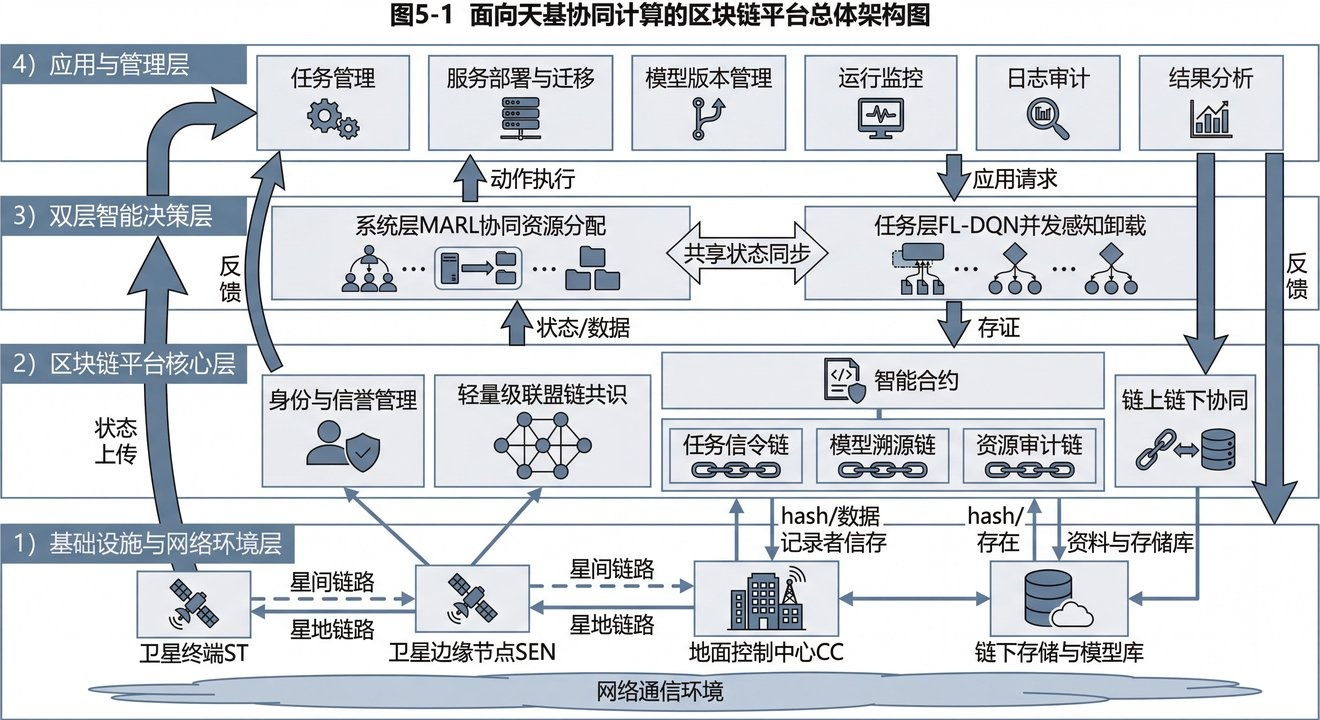
\includegraphics[width=0.96\textwidth]{figures/5-1.jpeg}
  \caption{面向天基协同计算的区块链平台总体架构图}
  \label{fig:platform-arch}
\end{figure}

在网络映射方面，平台将天基协同网络抽象为时变有向图，并据此区分共识维护节点与普通业务节点。定义时刻 $t$ 的天基协同网络为时变有向图
\[\mathcal{G}(t)=({\mathcal{V}},{\mathcal{E}}(t)),\]
其中，节点集合 $\mathcal{V}$ 表示参与天基协同计算与区块链维护的星地节点集合，边集合 $\mathcal{E}(t)$ 表示随时间变化的星间或星地通信连接关系。进一步将节点划分为负责区块打包、共识验证与全局状态定序的共识节点集合 $\mathcal{C}$，以及负责发起任务请求、状态上报和局部决策的普通节点集合 $\mathcal{L}$，满足
\[\mathcal{C}\subseteq \mathcal{V}, \qquad \mathcal{L}=\mathcal{V}\setminus \mathcal{C}.\]

进一步地，为避免平台层建模停留于纯粹的网络拓扑抽象，本文借鉴支撑项目中的天基网络试验任务调度思想，将平台中的任务—资源映射进一步表述为
\[\mathrm{SNEMS}=\{T,R,X,F\}\]
的四元组决策空间。其中，$T$ 表示待调度任务集合，$R$ 表示由平台集、载荷集、窗口集和执行时机构成的资源集合，$X$ 表示任务—资源决策矩阵，$F$ 表示由硬约束与收益函数构成的评价集合。该定义的作用不在于替代第2章的系统模型，而在于为第5章的平台化实现补充"任务如何进入区块链治理框架、资源如何进入系统层动作空间、局部决策如何受全局约束"的统一表达接口。

\textbf{分层链组织与运行接口。}
在平台运行过程中，不同类型的业务事件在频率、时延需求和安全等级方面存在明显差异。结合项目中已有的分层联盟链方案，平台将链结构划分为主链层、子链层和链下设备层。其中，主链负责任务调度、全局状态摘要、日志摘要及关键治理信息维护；子链负责特定区域、特定业务或特定任务类型的数据存证与协同；链下设备层负责原始数据、模型参数和大对象日志的缓存与对象化存储。

从节点角色看，平台可进一步区分为共识节点与非共识节点。主链共识节点负责区块打包、交易校验和全局广播；子链共识节点负责局部数据验证与存证；非共识节点主要承担任务接入、数据采集、状态上报和链下存储等功能。这一划分与项目中的主链—子链—边端设备设计保持一致，有助于在可信性与资源开销之间取得平衡。

进一步地，设平台在时刻 $t$ 的全局状态为 $S^{(t)}$，则在新区块 $B_h$ 经过共识确认后，平台可通过状态转移函数 $\Gamma(\cdot)$ 完成状态更新：
\[S^{(t+1)}=\Gamma\!\left(S^{(t)}, B_h, \Omega_{\text{rules}}\right),\]
其中，$\Omega_{\text{rules}}$ 表示平台治理规则与约束集合，其内部可映射第3章系统层协同策略所给出的全局资源边界、节点信誉约束和任务处理规则。

平台在区块链核心层之上提供统一的状态共享与约束传递接口。系统层输出的资源占用上界、节点可调度集合及链路可用区间，将作为任务层决策的外部约束输入；任务层在执行过程中产生的排队时延、任务成功率、资源消耗和异常事件等结果，则进一步回流至链上状态空间，为后续系统层迭代提供反馈依据。

在应用与管理侧，平台进一步提供任务管理、服务部署与迁移、模型版本管理、运行监控、日志分析、审计查询和策略展示等能力，为前文方法提供可观测、可分析和可配置的统一支撑环境。

\begin{figure}[htbp]
  \centering
  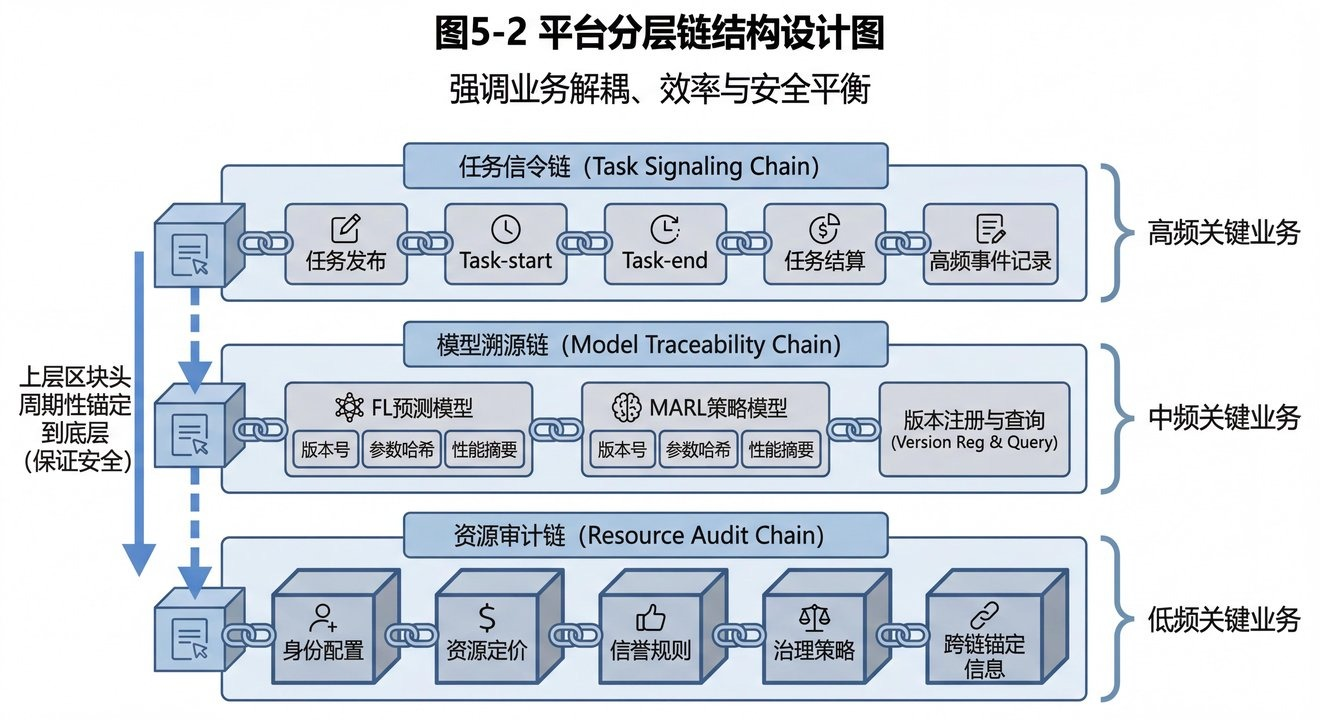
\includegraphics[width=0.92\textwidth]{figures/5-2.jpeg}
  \caption{平台分层链结构设计图}
  \label{fig:chain-arch}
\end{figure}

\section{区块结构、数据流转与存证机制}

\textbf{分层联盟链与链上/链下协同设计。}
传统公有链普遍采用工作量证明等高消耗共识机制，但该类机制难以适应天基网络环境下节点算力受限、能量预算紧张和业务时延敏感的实际约束。对于本文研究场景而言，平台更适合采用许可制联盟链结构，仅允许经过授权的卫星边缘节点、控制节点和少量高可信节点参与账本维护与交易验证，以减少无效竞争开销。

在具体机制选择上，权威证明和委托权益证明是两类较为适合的候选方案。权威证明依赖授权节点轮流出块，适合作为平台初始部署阶段的基础方案；委托权益证明则在保持较高效率的同时，引入代表节点选举机制，可结合节点信誉值、历史贡献度和服务能力动态调整记账节点集合，更适合平台进入稳定运行后的自治演进场景。

\textbf{区块结构与链上/链下协同。}
结合项目中的主链—子链设计，平台继承主链与子链的差异化区块结构。主链区块主要承载任务元数据、跨链摘要、治理规则、资源分配摘要与审计索引；子链区块主要承载业务域内的试验数据摘要、任务状态与局部日志记录。主链更强调调度与治理，子链更强调业务数据存证与局部协同。

在链上/链下协同方面，平台采用"链上保存摘要、链下保存实体对象"的分层管理方式。链上主要保存任务标识、状态摘要、模型版本哈希、审计索引、合约结果和关键治理规则等小体积但高价值的信息；链下则保存任务原始输入、完整模型参数、服务镜像和详细日志等大规模对象。链上记录通过哈希指针与链下对象建立映射关系，当节点需要访问链下数据时，可通过对比其哈希值验证对象的一致性与完整性。

结合项目文件中的分层联盟链与跨链网关设计，链上/链下协同机制还可进一步细化为"子链局部存证 + 主链摘要锚定"的双层存储流程。具体而言，任务执行过程中形成的原始数据、模型参数与详细日志首先保存在链下对象存储或边缘服务集群中，子链仅记录其哈希摘要和过程状态；跨链网关随后将子链摘要提交至主链进行全局锚定。

若记某一业务子链上的区块为 $B_s$，其保存的核心内容可抽象表示为
\[B_s=\{D_{\text{hash}},\, H(B_s^-),\, H(B_s)\},\]
主链在接收跨链网关提交的摘要后，将对应锚定区块记为
\[B_m=\{H(B_s),\, H(B_m^-),\, H(B_m)\}.\]
这一设计能够在不显著增加链上存储压力的前提下，为数据完整性与跨域可验证性提供密码学支撑。

\textbf{数据流转、存证流程与可信执行。}
在数据流转方面，平台沿用项目中"任务基础信息生成与广播—资源与数据信息管理—数据存储与验证—跨链接入与调度管理"的处理链路。具体而言，任务基础信息首先在主链层生成并广播，随后任务需求资源、试验数据和日志信息根据业务类型进入对应子链；大规模原始对象保存在链下，由子链记录摘要并通过跨链网关上传主链锚定。

进一步地，项目中的数据存证流程可为本章平台提供直接的工程实现参考。在数据写入过程中，客户端先向主链发起请求并完成身份与权限校验，随后由跨链网关按照路由转发至对应数据子链；子链完成写入后，将隐私数据哈希、存储位置和过程摘要回传主链存证。在数据读取过程中，主链先完成身份与权限确认，再由跨链网关访问对应子链并返回数据结果与哈希校验信息。由此，项目中的主链—子链—跨链网关—链下对象存储流程，正好为本章平台中的任务状态存证、模型版本锚定和执行日志回写提供了工程模板。

在分布式天基环境下，仅依赖人工配置和静态规则难以保证协同过程的持续稳定运行。为了将任务流转、模型治理和安全约束等关键逻辑由"人为约束"转化为"规则自动执行"，本文在平台中引入智能合约治理机制。任务管理合约用于完成任务注册、参数校验、任务接纳确认、执行开始记录、完成结果写回以及结算与奖惩触发；模型版本管理合约用于登记第4章联邦学习并发开销预测模型与第3章系统层策略模型的版本号、参数哈希、性能摘要和更新时间等内容。

进一步地，考虑到第4章中的联邦学习模型需要在多节点条件下持续演化，平台可将节点信誉值纳入模型聚合过程。即在完成本地训练后，各节点仅提交参数摘要、版本信息及必要的聚合索引，链下完成模型参数交换，链上则记录版本登记与合法性校验结果；对于信誉值持续偏低或存在异常行为的节点，其提交的聚合权重可被削弱或拒绝，从而增强模型治理的可靠性。

\section{双层智能方法的平台映射与运行闭环}

\textbf{系统层与任务层方法的平台映射。}
第3章提出的基于区块链与多智能体强化学习的系统层协同资源分配方法，主要面向全局尺度下的资源竞争与协同优化问题。在平台化实现中，该方法被映射为双层智能决策层中的系统层控制模块，其核心职责不再是单纯输出离线策略，而是持续接收链上共享状态并对全局资源边界进行动态更新。

具体而言，平台通过区块链核心层维护节点负载摘要、可用算力信息、链路质量指标、历史信誉状态以及任务分布统计结果等公共环境变量。系统层智能体在此基础上依据马尔可夫博弈框架进行策略更新，并形成资源分配建议、节点协同关系和服务能力边界等结果。这些结果并不直接替代任务层决策，而是以资源约束、候选集优先级和协同调度边界的形式向下传递。

在任务层，第4章提出的并发感知卸载方法被映射为局部实时决策模块，其输入由任务属性、本地节点状态、候选节点共享状态、系统层约束边界以及联邦学习模型预测结果共同构成。联邦学习预测模型的版本信息和参数摘要由模型版本管理合约统一维护，任务层节点在调用模型前可通过链上查询确认其版本合法性，并对模型参数进行哈希校验，从而保证预测输入来源可信。

\textbf{状态—动作—存证—反馈闭环。}
为了更清晰地描述平台中双层智能决策的运行逻辑，本文将平台核心流程抽象为"状态—动作—存证—反馈"闭环机制。设平台在时刻 $t$ 的联合状态表示为
\[S(t)=\{S_{\text{sys}}(t),\, S_{\text{task}}(t),\, S_{\text{chain}}(t)\},\]
其中，$S_{\text{sys}}(t)$ 表示系统层公共状态，$S_{\text{task}}(t)$ 表示任务层局部状态，$S_{\text{chain}}(t)$ 表示链上共享状态。

系统层根据联合状态生成资源协同动作 $a_{\text{sys}}(t)$，任务层结合局部状态与系统层约束生成卸载动作 $a_{\text{task}}(t)$。因此，平台在时刻 $t$ 的联合动作可表示为
\[A(t)=\{a_{\text{sys}}(t),\, a_{\text{task}}(t)\}.\]

在动作执行后，平台通过智能合约将关键行为记录为链上事件集合
\[E(t)=\{e_{\text{start}}(t),\, e_{\text{end}}(t),\, e_{\text{model}}(t),\, e_{\text{audit}}(t)\}.\]

在反馈阶段，任务执行所产生的时延、能耗、资源占用变化和任务完成质量等结果被汇聚为反馈向量 $F(t)$，并用于更新下一时刻的平台状态，即
\[S(t+1)=\Phi\!\left(S(t),A(t),E(t),F(t)\right).\]

\begin{figure}[htbp]
  \centering
  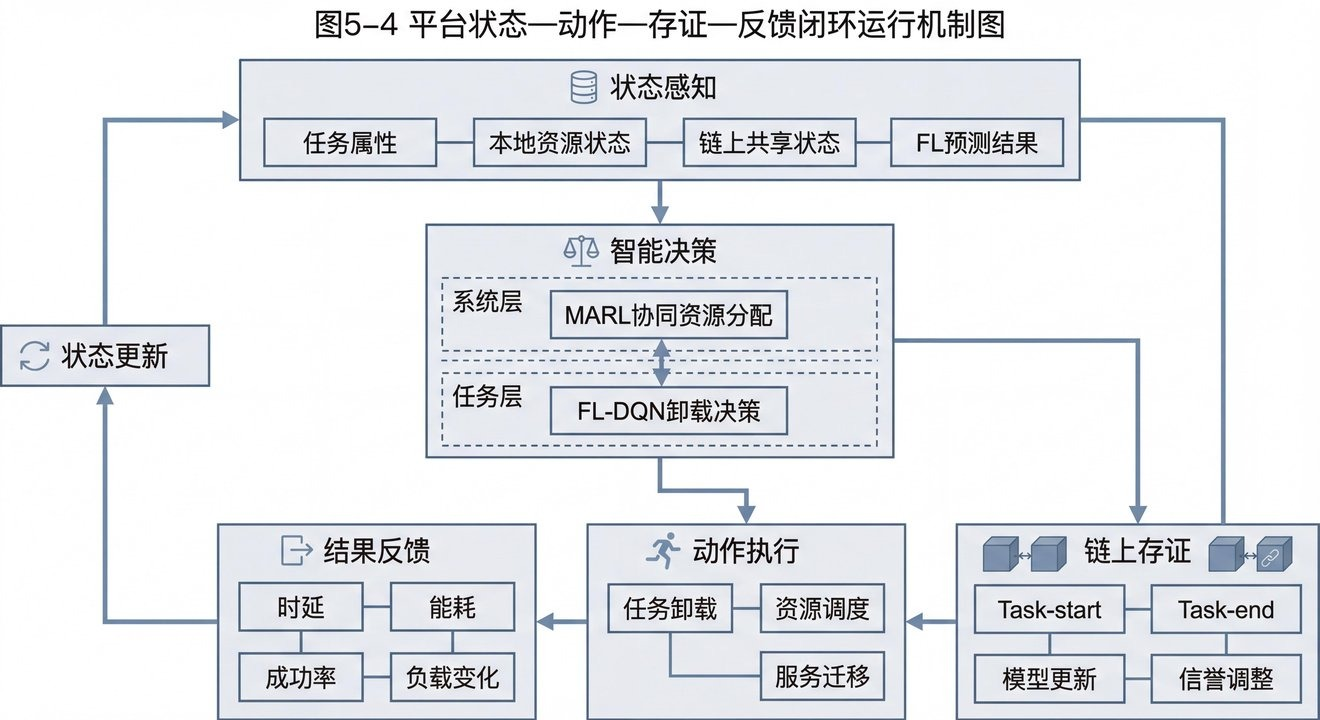
\includegraphics[width=0.92\textwidth]{figures/5-4.jpeg}
  \caption{平台状态—动作—存证—反馈闭环运行机制图}
  \label{fig:closed-loop}
\end{figure}

\textbf{资源审计、身份控制与信誉评估。}
第3章提出的系统层多智能体强化学习方法输出的是全局资源协同结果，而第4章任务层方法则面向单任务到达瞬间做出局部动作选择。为了避免两层决策彼此割裂，平台需要建立从系统层到任务层的约束传递机制。为此，平台可将系统层输出的协同动作表示为 $A_{\text{sys}}$，并进一步映射为面向任务层的局部约束集合 $C_{\text{limit}}$。当单任务到达并触发任务层深度强化学习决策时，其可行动作空间可表示为
\[A'_{\text{task}}=A_{\text{task}}\cap C_{\text{limit}}.\]

在身份认证方面，平台采用联盟链白名单准入机制，仅允许经过授权的节点参与网络；并通过数据访问授权与合约调用授权，限制不同角色对任务信息、试验数据、模型版本与治理合约的操作权限。该部分直接继承了项目中已有的身份管理与访问控制思路。

在资源审计与信誉评估方面，平台持续记录节点的资源声明、任务接纳情况、实际执行结果和历史服务质量，并结合审计规则对其一致性进行检查。设节点 $i$ 在时间窗 $\tau$ 内的信誉值为 $R_i(\tau)$，则其更新可表示为
\[R_i(\tau)=\alpha R_i(\tau-1)+(1-\alpha)\sum_{k\in T_i} I(\text{link}_k)\,\omega_k\,\varphi(k),\]
其中，$\alpha\in(0,1)$ 为历史遗忘因子，$\omega_k$ 为任务重要度权重，$\varphi(k)$ 表示任务 $k$ 的执行评价项，$I(\text{link}_k)$ 为链路状态感知因子，用于刻画任务执行期间对应星间或星地链路是否处于可见且可通信状态。

\section{平台运行流程、工程分析与本章小结}

\textbf{平台运行流程。}
为进一步展示平台的数据流转机制，本节结合灾害应急多星协同计算场景，对双层智能方法在平台中的运行逻辑进行说明。系统初始阶段，各卫星节点同步包含全局负载摘要与模型版本哈希的最新区块头，并结合本地缓存完成运行状态初始化。当高密度遥感图像识别任务在某一低轨卫星节点产生后，任务层首先提取局部状态，并从链下模型库获取当前有效模型参数，通过模型版本管理合约完成哈希一致性校验。在模型合法性得到确认后，任务层深度强化学习模块输出具体卸载动作。

随后，任务请求进入平台合约处理流程。跨层约束机制将依据系统层资源协同结果判断目标节点是否仍处于允许接纳任务的资源边界之内。若满足约束条件，则平台生成任务开始事件并记录相应状态；若不满足，则任务需重新选择候选节点或回退至本地执行。待任务执行结束后，系统将时延、能耗和完成质量等结果封装为反馈信息写回平台，并同步完成链上存证、信誉结算和样本沉淀。

模型更新与版本治理过程中，各节点基于本地任务样本开展联邦训练，聚合后的新模型由版本管理合约登记其版本号、参数哈希与性能摘要。平台还可在检测到局部区域出现任务热点、节点拥塞或服务失衡时，触发服务部署与迁移流程，以保持系统能力分布的动态均衡。

\textbf{平台项目对前文方法的支撑作用。}
从全文结构看，本章引入平台项目的目的，在于把前文分散于模型、算法和决策层的研究内容串联起来。第2章给出了天基协同计算的系统模型与状态约束，第3章提出了基于区块链与多智能体强化学习的系统层协同资源分配方法，第4章提出了基于联邦学习与深度强化学习的任务层并发感知卸载方法；而本章则依托项目中已完成的分层联盟链、主链—子链区块结构、跨链网关、数据流转与存证流程、以及身份与访问控制等设计，为这些方法提供统一的工程承载环境。

\textbf{工程可行性分析。}
为进一步验证本文所设计区块链平台架构在天基动态环境下的可行性，本文结合 STK 生成星座轨道与可见性关系，并利用 NS-3 构建网络层通信仿真环境。仿真重点关注平台在共识开销、存储增长和异常节点隔离等方面的运行特性，以检验平台对前文双层智能方法的承载能力。

评估指标主要包括确认时延、存储开销增长以及信誉驱动的异常节点隔离效果等。通过上述配置，可以从"吞吐与时延""存储可持续性""异常治理能力"三个维度对平台工程适应性进行考察。综合结果表明，平台在吞吐能力、确认时延、存储控制和异常治理等方面均表现出较好的工程适应性。

\textbf{本章小结。}
综合上述分析可以看出，本章所设计的平台并非对前文算法的简单附属说明，而是依托已完成的平台项目，将系统建模、系统层协同优化与任务层实时决策统一到一个可运行、可验证、可审计的工程框架中。其中，项目中已有的分层联盟链、主链—子链区块结构、跨链网关、数据流转与存证流程、以及身份与访问控制等设计，为平台的可信状态同步、任务行为存证、模型版本治理和执行反馈闭环提供了直接支撑；而第3章和第4章提出的双层智能方法，则在这一平台上完成了从算法层到系统层的落地映射。由此，本文实现了从系统模型、算法设计到平台实现的研究链条闭合，也使第五章真正承担起"用平台项目把前几章串起来"的作用。

\backmatter

%%
% BIThesis 研究生学位论文模板 The BIThesis Template for Graduate Thesis
% This file has no copyright assigned and is placed in the Public Domain.
%%

\chapter{结论与展望}
\label{chap:conclusion}

随着天地一体化信息网络、低轨卫星星座和在轨智能处理技术的发展，天基网络正在由传统的数据传输网络向集通信、计算、存储和智能处理于一体的分布式协同计算网络演进。在灾害应急通信、遥感快速处理、空间态势感知、区域目标识别和边远区域信息服务等典型场景中，天基网络不仅需要完成数据采集与远程传输，还需要在星地链路受限、星间拓扑高动态、节点资源异构和任务负载突发变化的条件下，实现任务接入、资源协调、计算处理与结果反馈的快速闭环。然而，传统星地集中处理模式容易受到星地链路时延、可见窗口和回传带宽限制，单星本地处理模式又受限于星载平台的算力、能量、功耗和存储资源，难以持续支撑高并发、高时敏和高自治要求的计算任务。因此，如何在高动态、资源受限和去中心化的天基网络环境中，实现可信、高效的多星协同计算卸载，成为提升天基网络智能服务能力的重要问题。

本文围绕高动态天基网络中的可信协同计算卸载问题，按照“统一建模—系统层协同—任务层卸载”的研究主线展开。首先，构建包含动态网络、异构资源、任务生命周期和区块链账本可信状态共享的统一建模框架，并将总体问题分解为系统层协同资源分配和任务层并发开销感知卸载两个子问题；随后，分别设计基于区块链与多智能体强化学习的系统层协同资源分配方法，以及基于聚类联邦学习与DQN的任务层实时卸载方法，从而形成由统一建模支撑、双层方法展开、执行反馈闭环更新的研究体系。全文主要研究工作总结如下。

（1）构建了天基网络可信协同计算卸载统一建模框架。针对天基网络中节点异构、链路时变、任务随机到达和状态共享可信性不足等问题，本文建立了包含卫星终端、卫星边缘节点、地面控制中心和区块链账本的协同计算模型，分别刻画了网络拓扑、节点资源、任务属性、链路传输、本地计算、星间卸载、能耗开销和并发开销等关键要素。在此基础上，本文将区块链账本抽象为可信状态共享与反馈机制，通过链上摘要与链下实体数据分离的方式维护节点状态摘要、任务生命周期记录、节点信誉和模型版本凭据。进一步地，本文建立了统一协同计算卸载优化目标，并将其分解为系统层协同资源分配子问题和任务层并发开销感知卸载子问题，为后续章节提供了统一符号体系、状态接口和问题边界。

（2）提出了基于区块链与多智能体强化学习的系统层协同资源分配方法。针对去中心化天基计算网络中节点能力异构、任务到达非平稳、链路状态动态变化以及节点自利行为导致的资源竞争和负载失衡问题，本文将系统层协同资源分配问题建模为多智能体马尔可夫博弈，并提出区块链增强的集中训练—分散执行多智能体强化学习框架。该方法利用联盟链作为可信公共信息板，维护节点负载、链路状态、信誉评分和历史行为记录等系统级公共摘要，在不依赖长期稳定中心控制器的条件下，为各卫星节点提供可验证、可追溯的协同上下文。同时，本文设计了融合任务完成质量、系统公平性和信誉激励的混合奖励函数，引导自利节点在长期交互中形成更接近系统最优的协同策略。仿真实验表明，该方法能够提升任务完成率和系统吞吐量，改善负载均衡效果，并增强系统对自利行为和不完全信息环境的适应能力。

（3）提出了基于聚类联邦学习与DQN的并发感知任务层计算卸载方法。在系统层实现可信协同的基础上，本文进一步关注任务到达瞬间的节点侧实时卸载决策问题。针对多任务并发执行过程中 CPU 时间片、缓存、内存带宽和 I/O 队列竞争所导致的隐性并发开销，本文建立了任务级并发开销建模方法，将新任务自身计算时延和存量任务剩余时延增加统一纳入任务层代价模型。考虑到天基网络中任务执行日志不适合集中上传、节点数据分布具有明显 Non-IID 特征、区块链账本维护的可信公共摘要存在时滞等问题，本文提出了“聚类式联邦学习预测 + DQN 卸载决策”的闭环机制。该方法通过聚类式联邦学习在不共享原始任务数据的前提下训练并发开销预测模型，并通过区块链账本维护并发开销预测模型版本和可信摘要；随后将预测结果、本地观测状态和区块链账本维护的可信公共摘要共同输入深度 Q 网络，实现低开销、实时化且具备并发开销前瞻能力的任务卸载决策。实验结果表明，该方法能够有效降低高并发场景下的任务时延和能耗，提高任务完成率与系统稳定性。

综上，本文面向天基网络中的可信协同计算卸载需求，形成了由统一建模、系统层协同资源分配和任务层并发开销感知卸载构成的方法体系。研究表明，区块链账本能够为去中心化天基网络提供可信状态共享、任务生命周期记录、信誉维护和并发开销预测模型版本管理能力；多智能体强化学习能够有效支撑系统层多节点协同资源分配；聚类式联邦学习与DQN的结合能够在隐私受限、状态滞后和负载异构条件下提升任务层卸载决策的实时性与准确性。相关研究可为未来构建高效、智能、可信的天基边缘计算网络提供理论依据和方法支撑。

在本文研究基础上，仍有以下方向值得进一步深入探索。

（1）更真实轨道与链路环境下的模型验证。本文主要通过仿真方式验证所提方法，后续可结合真实星座轨道数据、星间链路测量数据和任务负载数据，对模型进行进一步校准。同时，可引入更精细的轨道动力学模型、星间链路中断模型、太阳能充放电模型、热控约束模型和多业务混合到达模型，使统一建模更加贴近真实星座运行环境。

（2）面向大规模星座的轻量化协同优化。随着节点规模扩大，多智能体训练复杂度、区块链账本维护的可信公共摘要维护开销和候选节点筛选成本将进一步增加。后续可研究图神经网络、参数共享、分层策略、模型压缩和边缘推理加速等方式提升可扩展性，使系统能够在更大规模星座中保持较低通信开销和较高协同效率。

（3）区块链可信机制与实时卸载决策的深度融合。本文将区块链主要用于状态摘要、任务生命周期记录、信誉维护和模型版本管理，后续可进一步研究更轻量的共识机制、跨链状态压缩方法、面向时敏任务的可信状态快速确认机制以及链上事件与强化学习奖励之间的自适应耦合方法，从而在可信性和实时性之间取得更优平衡。

\input{./misc/2_reference.tex}
%%
% BIThesis 研究生学位论文模板 The BIThesis Template for Graduate Thesis
% This file has no copyright assigned and is placed in the Public Domain.
%%

\begin{appendices}
  \chapter{仿真参数与环境配置}

  本附录用于补充正文实验部分未展开列出的参数设置与环境说明，便于对本文方法的实验条件进行统一说明与后续复现实验。实验环境主要围绕天基网络计算卸载场景进行构建，涉及卫星终端、卫星边缘节点、链路参数、任务到达过程以及算法超参数等多个方面。对于不同实验场景，可在统一参数基线的基础上对节点规模、任务强度、链路时延与负载水平进行适当调整。

  在系统参数设置方面，可重点说明卫星节点数量、节点计算能力范围、任务输入规模、任务计算量分布、链路带宽区间、传播时延范围以及任务时延约束设置等内容；在算法参数设置方面，可进一步补充多智能体强化学习、联邦学习与深度强化学习相关的学习率、折扣因子、训练轮数、批大小与聚合周期等参数。对于实验中使用的评价指标，如平均时延、任务完成率、系统吞吐量、负载均衡度和能耗等，也可在附录中统一列出其统计口径与计算方式。

  \chapter{关键模型推导与补充说明}

  本附录用于补充正文中为保持行文紧凑而未详细展开的模型推导过程与符号说明。针对系统层协同资源分配问题，可进一步给出状态变量、动作变量、奖励函数各分量以及约束条件之间的对应关系；针对任务层并发感知卸载问题，可补充并发开销定义、工程近似表达及其与综合代价函数之间的推导联系。

  此外，对于文中涉及的关键符号、参数物理意义与公式适用条件，也可在本附录中进行集中说明，以增强模型表达的一致性与可读性。当后续章节补充完整实验内容后，本附录还可进一步加入复杂度分析、敏感性分析推导或部分中间证明过程，以形成与正文相互支撑的完整结构。

  \chapter{附录内容说明}

  附录部分主要用于补充不宜在正文中大篇幅展开、但对理解论文研究过程和复现实验结果具有参考价值的材料。其内容通常包括但不限于以下几类：
  \begin{enumerate}
    \item 正文中为保证结构紧凑而省略的详细模型推导、符号说明与中间证明过程；
    \item 实验平台配置、参数设置、数据生成规则与评价指标统计口径等支撑性材料；
    \item 关键算法流程、训练细节、补充结果或扩展对比分析；
    \item 对同行读者具有参考意义、但不适合直接纳入正文主体的技术性补充内容。
  \end{enumerate}

  \section{附录内容组织说明}

  为便于后续完善，附录可按照“实验参数补充—模型推导补充—结果说明补充”的结构逐步补全，并与正文中对应章节保持编号和引用关系的一致性。

  \subsection{后续补充建议}

  随着第五章、第六章内容的进一步完善，可将更具体的仿真参数表、额外实验图表及推导细节逐步整理至本附录中，以增强全文结构的完整性与学术表达的规范性。
\end{appendices}

\input{./misc/4_pub.tex}

\end{document}
